%-  LaTeX source file

%-  main.tex ~~
%
%   This is the "main" document file, which means it is the one that will
%   \include all the other source files.
%
%                                                   ~~ last updated 25 Sep 2019

%%%%%%%%%%%%%%%%%%%%%%%%%%%%%%%%%%%%%%%%%%%%%%%%%%%%%%%%%%%%%%%%%%%
%
% This is a general template file for the LaTeX package SVJour3
% for Springer journals.          Springer Heidelberg 2010/09/16
%
% Copy it to a new file with a new name and use it as the basis
% for your article. Delete % signs as needed.
%
% This template includes a few options for different layouts and
% content for various journals. Please consult a previous issue of
% your journal as needed.
%
%%%%%%%%%%%%%%%%%%%%%%%%%%%%%%%%%%%%%%%%%%%%%%%%%%%%%%%%%%%%%%%%%%%
%
\RequirePackage{fix-cm}
%
%\documentclass{svjour3}                     % onecolumn (standard format)
%\documentclass[smallcondensed]{svjour3}     % onecolumn (ditto)
\documentclass[smallextended]{svjour3}      % onecolumn (second format)
%\documentclass[draft,smallextended]{svjour3} % second format in draft mode
%\documentclass[twocolumn]{svjour3}          % twocolumn

\smartqed  % flush right qed marks, e.g. at end of proof

\usepackage{graphicx}
\usepackage{amsmath}
\usepackage{hyperref}
\usepackage{listings}
\usepackage{algorithm}
\usepackage[noend]{algpseudocode}

\begin{document}

\title{Improving Resource Utilization by High-throughput Workload Management
on Leadership Class Facilities~\thanks{\textcolor{blue}{%
Grants or other notes about the article that should go on the front page should
be placed here. General acknowledgments should be placed at the end of the
article.}}
}
\subtitle{\textcolor{blue}{Do you have a subtitle?\\ If so, write it here}}

%\titlerunning{Short form of title}        % if too long for running head

\author{%
    Sean R.\ Wilkinson~$^1$ \and
    Danila Oleynik~$^2$ \and
    Ruslan Mashinistov~$^3$ \and
    Andre Merzky~$^4$ \and
    Sergey Panitkin~$^3$ \and
    Pavlo Svirin~$^5$ \and
    Matteo Turilli~$^4$ \and
    Kaushik De~$^5$ \and
    Alexei Klimentov~$^3$ \and
    Shantenu Jha~$^{3, 4}$ \and
    Jack C.\ Wells~$^1$
}

\authorrunning{Sean R.\ Wilkinson et al.} % if too long for running head

\institute{%
    $^1$~Oak Ridge National Laboratory,
        Oak Ridge, Tennessee, USA \\
    $^2$~Joint Institute for Nuclear Research,
        Dubna, Moscow Oblast, Russia \\
    $^3$~Brookhaven National Laboratory,
        Upton, New York, USA \\
    $^4$~Rutgers, the State University of New Jersey,
        New Brunswick, New Jersey, USA \\
    $^5$~University of Texas at Arlington,
        Arlington, Texas, USA
%    S. Wilkinson \at Oak Ridge National Laboratory \\
%        \email{wilkinsonsr@ornl.gov}
%              first address \\
%              Tel.: +123-45-678910\\
%              Fax: +123-45-678910\\
%              \email{fauthor@example.com}           %  \\
%%             \emph{Present address:} of F. Author  %  if needed
%           \and
%           S. Author \at
%              second address
}

\date{Received: date / Accepted: date}
% The correct dates will be entered by the editor

\maketitle

% ---------------------------------------------------------------------------
% ABSTRACT
% ---------------------------------------------------------------------------

\begin{abstract}
Large experiments and big science projects have historically used distributed
resources to meet their computing requirements. On the other hand, leadership
class machines have traditionally been utilized for workloads with very
distinct properties, namely, large MPI jobs. Given this gap, two interesting
questions are: can leadership computing facilities support workloads that
historically used distributed high-throughput resources? Can workload
management systems that were designed and implemented to support distributed
high throughput computing (HTC) support the efficient execution of workloads
on leadership class platforms? This paper documents our experience in enabling
PanDA --- Production and Distributed Analysis (PanDA) originally developed for
the ATLAS experiment at the Large Hadron Collider (LHC) at CERN, as a
production workload management on Titan --- a leadership class machine that
operated from 2012-2019. PanDA was modified to interact with the Moab resource
manager in two distinct operational modes: a ``batch queue mode'' that used
traditional allocations, and a ``backfill mode'' that opportunistically
consumed otherwise unutilized resources. For the traditional mode, new
techniques were implemented to shape large jobs for consuming allocations on a
leadership-class machine. In backfill mode, workloads was executed as backfill
to high priority leadership-class jobs but the stated goal of utilizing
resources without impacting Titan's quality of service as experienced by other
jobs. We propose several metrics by which to measure the impact; our analysis
suggests that with high probability and degree of confidence, the ATLAS
project was able to utilize 420 million core hours in backfill mode without a
discernible impact on other jobs and also increased the overall utilization of
Titan. Finally, we describe the use of PanDA for experiments in other
scientific fields such as astronomy, genomics, and neuroscience, using both
OLCF resources and other HPC resources.
\keywords{ATLAS \and HTC \and HPC \and PanDA \and OLCF \and Titan \and WMS}% \PACS{PACS code1 \and PACS code2 \and more}
% \subclass{MSC code1 \and MSC code2 \and more}
\end{abstract}

% The Production and Distributed Analysis (PanDA) software was originally
% developed as a High Throughput Computing (HTC) workload management system (WMS)
% on distributed grid resources for the ATLAS experiment at the Large Hadron
% Collider (LHC) at CERN. The BigPanDA team extended PanDA to access High
% Performance Computing (HPC) resources, allowing leadership-class supercomputers
% like Titan at Oak Ridge Leadership Computing Facility (OLCF) to become grid
% sites for the Worldwide LHC Compute Grid (WLCG). ATLAS consumed more than 620
% million Titan core hours from 2016-2018 as part of its production workflow for
% simulations by extending PanDA to interact with the Moab resource manager in
% two distinct operational modes: a ``batch queue mode'' that used traditional
% allocations to consume 200 million core hours, and a ``backfill mode'' that
% opportunistically consumed unutilized resources totaling more than 420 million
% core hours. For the traditional mode, new techniques were implemented to shape
% large jobs for consuming allocations on a leadership-class machine. In backfill
% mode, work was streamed steadily to Titan to backfill high priority
% leadership-class jobs, with the goal of consuming unutilized resources that
% would have otherwise remained unutilized, without affecting other projects'
% quality of service. This goal was evaluated with several studies that are
% included here, and the studies concluded that the goal was achieved. Finally,
% this report describes the use of PanDA for experiments in other scientific
% fields. Multiple demonstration workflows are described for fields such as
% astronomy, genomics, and neuroscience, using both OLCF resources and other HPC
% resources. 

% ---------------------------------------------------------------------------
% I - INTRODUCTION
% ---------------------------------------------------------------------------

\section{Introduction}
\label{sec:introduction}
%-  LaTeX source file

%-  section1.tex ~~
%                                                   ~~ last updated 24 Sep 2018

The Production and Distributed Analysis (PanDA) software was originally
developed as a High Throughput Computing (HTC) workload management system (WMS)
on distributed grid resources for the ATLAS experiment at the Large Hadron
Collider (LHC) at CERN. Traditionally, the ATLAS experiment at LHC has utilized
distributed resources as provided by the Worldwide LHC Compute Grid (WLCG) to
support data distribution and enable the simulation of events. The WLCG is the
world's largest computing grid, boasting more than 1 million computer cores and
1 exabyte of storage combined from more than 170 individual computing centers
in 42 countries. ATLAS experiment uses this geographically distributed grid to
process, simulate, and analyze its data, which total more than 350 petabytes.
After the early success in discovering a new particle consistent with the
long-awaited Higgs boson, ATLAS continued taking the precision measurements
necessary for further discoveries during Run 2, which came to an end in
December 2018. Especially in light of the future Run 3 as well as the High
Luminosity LHC (HL-LHC) project, it is obvious that the need for simulation and
analysis will overwhelm the expected capacity of WLCG computing facilities
unless the range and precision of physics studies are curtailed.

Over the past few years, the ATLAS experiment has been investigating the
implications of using high-performance computers -- such as those found at Oak
Ridge Leadership Computing Facility (OLCF) and other United States Department
of Energy (DOE) computing facilities -- to augment WLCG computing facilities by
integrating their High Performance Computing (HPC) resources. This steady
transition is a consequence of application requirements such as greater than
expected data production, as well as technology trends and software complexity.

To this end, the BigPanDA team extended PanDA to access HPC resources, allowing
leadership-class supercomputers like Titan at OLCF to become grid sites for the
WLCG. HPC resources are not necessarily tuned for processing data on the scale
of the ATLAS experiment, but they are incredibly well-suited for simulation
work. Taking advantage of the strengths of HPC resources like Titan allowed
ATLAS to consume more than 620 million Titan core hours during the three years
from 2016-2018 as part of its production workflow for simulations. Not only did
this represent a large proportion of ATLAS's resource consumption for
simulations, but it also led to the incorporation of other DOE HPC resources as
WLCG grid sites, including Theta at the Argonne Leadership Computing Facility
(ALCF) and Cori at the National Energy Research Scientific Computing Center
(NERSC).

Here, we describe the architectural, algorithmic, and software changes which
were addressed in order to prepare the PanDA WMS for the exascale. We will
focus on our experiences in adapting PanDA to work with Titan at the OLCF. Even
though Titan was decommissioned in August 2019, these experiences are directly
applicable to Summit, OLCF's pre-exascale successor to Titan. In particular, we
will discuss the extensions to PanDA that allowed it to interact with Titan's
Moab resource manager in two distinct operational modes: a ``batch queue mode''
that used traditional allocations to consume 200 million core hours, and a
``backfill mode'' that opportunistically consumed unutilized resources totaling
more than 420 million core hours. For the traditional mode, we will describe
new techniques that were implemented to shape large jobs for consuming DOE
Advanced Scientific Computing Research (ASCR) Leadership Computing Challenge
(ALCC) allocations on Titan.

We also describe the use of a ``backfill mode'' for PanDA in which work was
streamed steadily to Titan and reshaped and submitted dynamically based on
available unutilized resources. The BigPanDA team took advantage of the
backfill scheduling feature of the Moab resource manager with the goal of
consuming unutilized resources that would have otherwise remained unutilized,
without affecting other projects' quality of service. We assess the
performance of PanDA with respect to this goal with several studies that are
included here.

Finally, this report describes the use of PanDA for experiments in other
scientific fields. Multiple demonstration workflows are described for fields
such as astronomy, genomics, and neuroscience, using both OLCF resources and
other HPC resources.

%-  vim:set syntax=tex:


% ---------------------------------------------------------------------------
% II - PanDA Workload Management System: Software System Overview
% ---------------------------------------------------------------------------

\section{PanDA Workload Management System: Software System Overview}
\label{sec:overview}
PanDA is a Workload Management System (WMS)~\cite{marco2009glite} designed to
support the execution of workloads in grid-like distributed computing
environment via pilots~\cite{turilli2017comprehensive}. A pilot-capable WMS
enables high throughput of task execution via multi-level scheduling while
supporting interoperability across multiple sites. This is particularly
relevant for Large Hadron Collider (LHC) experiments, where millions of tasks
are executed across more than 170 sites of the Worldwide LHC Computing Grid
(WLCG) every month, analyzing and producing petabytes of data. The design of
PanDA WMS started in 2005 to support ATLAS.

% ---------------------------------------------------------------------------
\subsection{Design}
\label{subsec:design}

PanDA's application model renders workloads into tasks which are decomposed
into jobs. Workloads are sets of data and transformations for the data. Tasks
are sets of homogeneous operations performed on data stored in sets of input
files. Tasks are decomposed into jobs, where each job consists of the task's
operations performed on a partition of the task's data. Jobs are distributed
across the available compute resources for concurrent execution.

PanDA's data model has been exclusively motivated by the needs of ATLAS, where
each datum refers to a recorded or simulated measurement of a physical process.
Data are stored in files that are grouped into datasets, with a many-to-many
relationship between files and datasets. Data have both attributes and states.
Raw, reconstruction, and simulation data are all assumed to be distributed
across multiple storage facilities and managed by the ATLAS Distributed Data
Management (DDM)~\cite{garonne2012atlas}. Files required by jobs are assumed to
be replicated over the network as needed, both for input and output data. PanDA
supports provenance and traceability for jobs and data. Attributes enable
provenance by linking jobs and data items, providing information like ownership
or project affiliation. States enable traceability by providing information
about the past and present stages of the execution for each job and data file.

%As with jobs, data have both attributes and states, and some of the attributes
%are shared among events and jobs.

PanDA's execution model is based on four main abstractions: tasks, jobs,
queues, and pilots. Both tasks and jobs are assumed to have attributes and
states and to be queued into a global queue for execution. Prioritization and
binding of jobs are assumed to depend on the attributes of each task and job.
PanDA has one global queue where all jobs are registered and one resource queue
for each target compute resource. PanDA assigns specific sets of jobs from
the global queue to the resource queues, depending on the jobs' requirements
and each resource's capability and availability. When pilots become available
on the target compute resource, PanDA sends jobs on each pilot from the
resource queue associated with that target compute resource.

PanDA's security model is based on separation among authentication,
authorization, and accounting for both single users and groups of users. Both
authentication and authorization are based on digital certificates and on the
virtual organization abstraction~\cite{foster2001anatomy}. 


% ---------------------------------------------------------------------------
\subsection{Implementation and Execution}
\label{subsec:implementation}

The implementation of PanDA WMS consists of several interconnected
subsystems, most of them built from off-the-shelf and Open Source components.
Subsystems communicate via messaging using HyperText Transfer Protocol (HTTP)
and dedicated Application Programming Interfaces (APIs), and each
subsystem is implemented by one or more modules. Databases are used to store
tasks, jobs, input/output data, and information about WLCG sites and compute
resources.

Currently, PanDA's architecture has five main subsystems:
AutoPyFactory~\cite{caballero2012autopyfactory},
JEDI/PanDA Server~\cite{maeno2011overview,borodin2015scaling},
PanDA Monitoring~\cite{klimentov2011atlas},
PanDA Pilot~\cite{nilsson2011atlas}, and Schedconfig~\cite{nilsson2008panda}.
AutoPyFactory is the system used to submit pilots to grid sites. JEDI and PanDA
Server process tasks into jobs and broker their distributed execution. PanDA
Monitoring is a web application to monitor the execution of workloads in a
distributed computing environment. PanDA Pilot is a pilot system that executes
jobs on computing infrastructures, managing the stage-in and stage-out of the
jobs' data. Schedconfig is an information system implemented within PanDA to
store PanDA queue (resource) descriptions. Schedconfig synchronizes with the
ATLAS Grid Information system (AGIS)~\cite{anisenkov2014agis} to obtain
information about distributed resources. Other subsystems are used by some
ATLAS workflows (e.g., ATLAS Event Service~\cite{calafiura2015atlas} and ATLAS
Production System~\cite{borodin2016atlas}), but their discussion is omitted
here because they are irrelevant to understanding how PanDA has been ported to
supercomputers. For a full list of subsystems, see Ref.~\cite{panda-wiki_url}.

Figure~\ref{fig:architecture} shows a diagrammatic representation of PanDA's
main subsystems, highlighting the task execution process while omitting
monitoring details to improve readability. During the first data collection
period at the LHC (LHC Run 1), PanDA required users to perform a static
conversion between tasks and jobs; tasks were described as a set of jobs and
then submitted to the PanDA Server. This introduced inefficiency both with
usability and resource utilization. Ideally, users should conceive analyses in
terms of one or more potentially related tasks, while the workload manager
(i.e., PanDA) should partition tasks into jobs, depending on the amount of data
(i.e., number of input files and events) that need to be processed and the task
requirements.

\begin{figure*}
  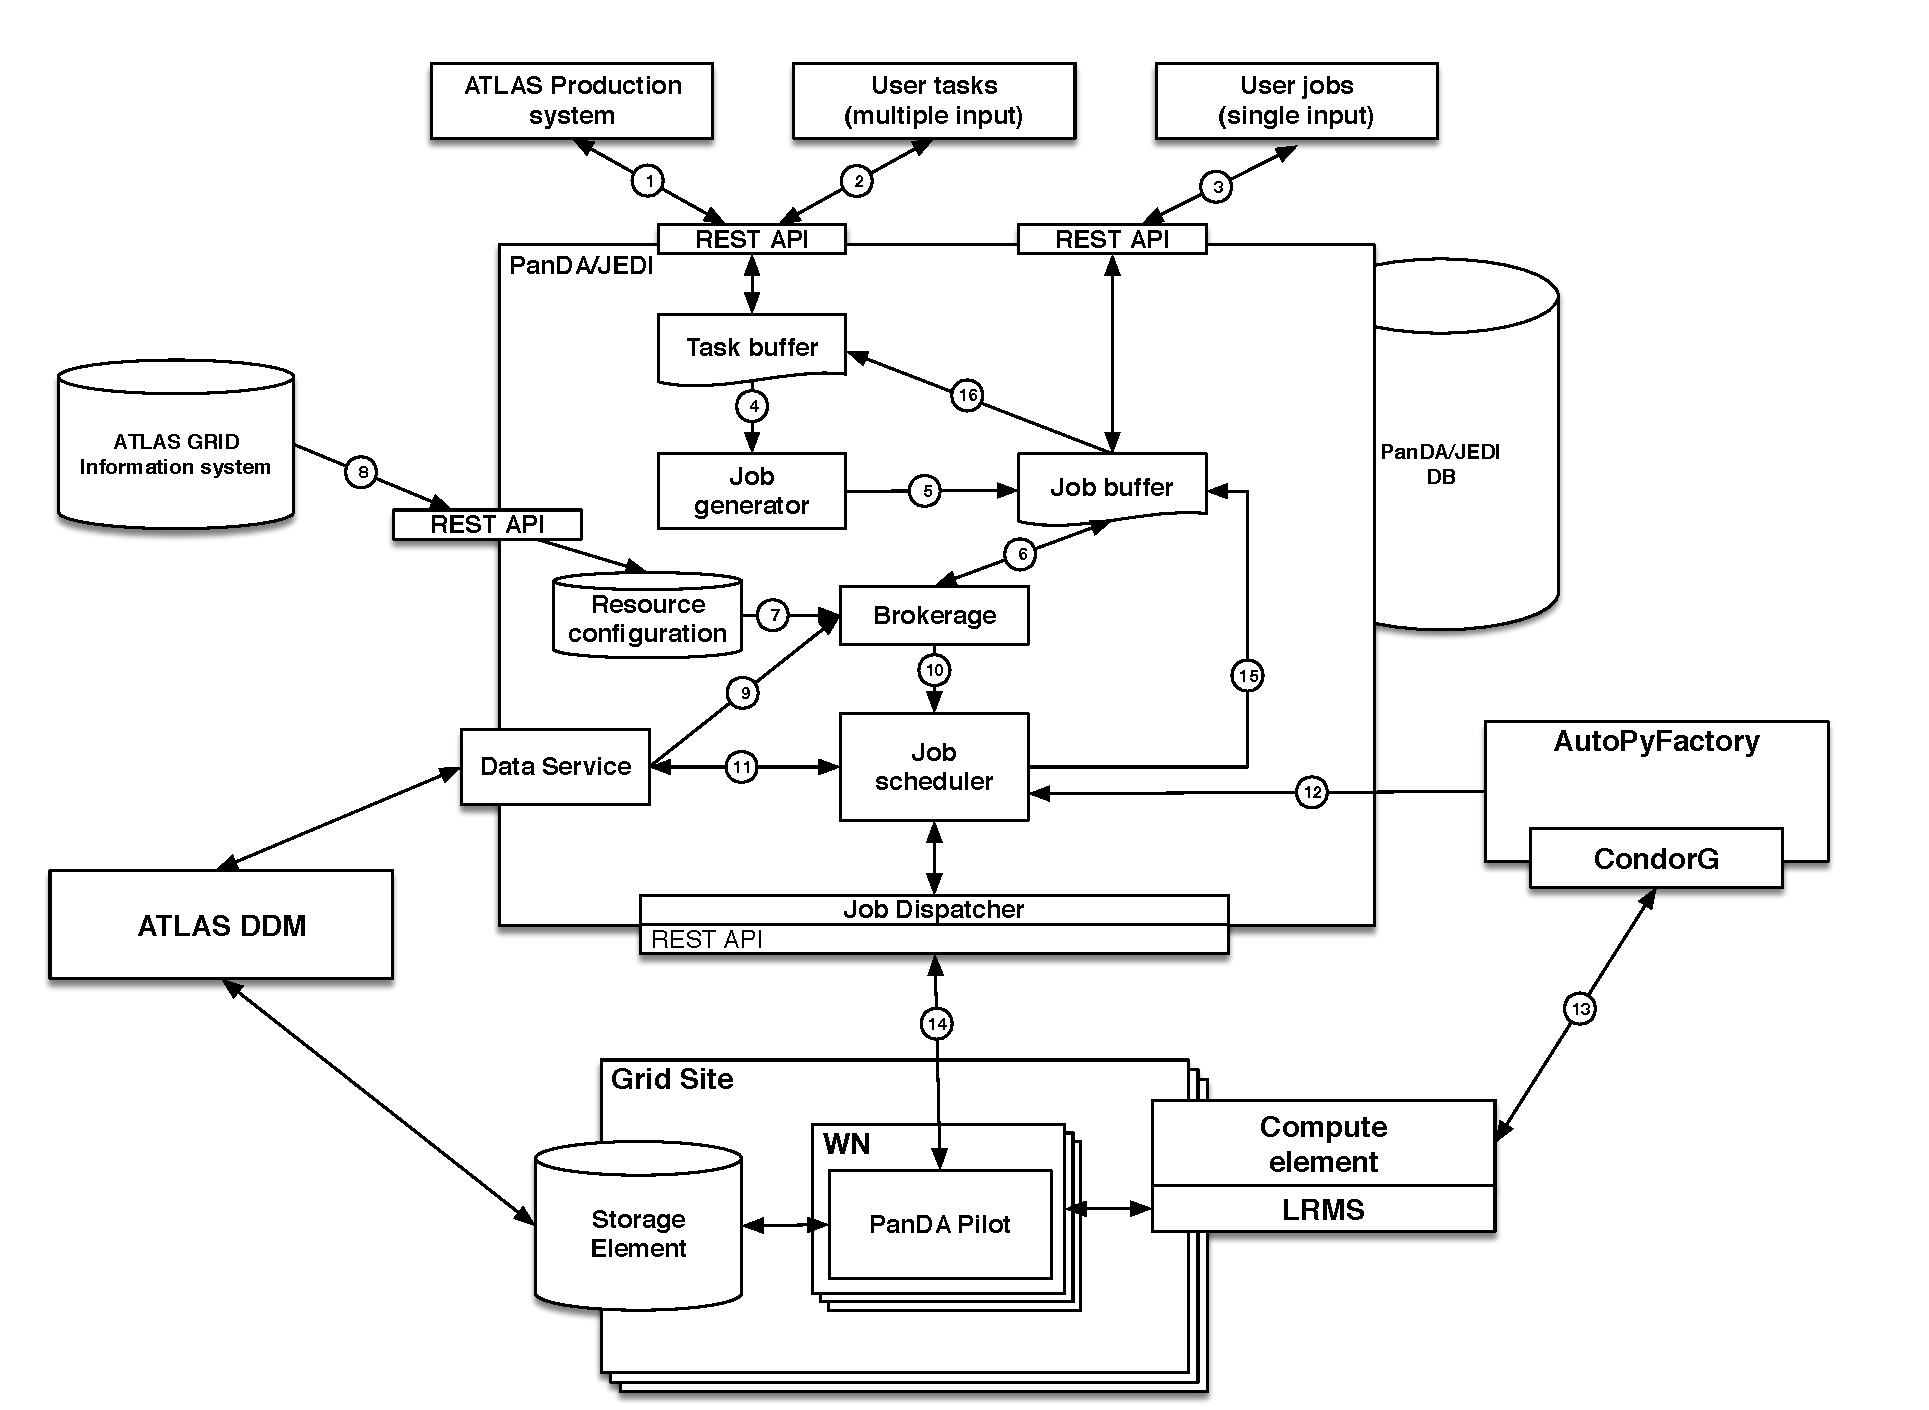
\includegraphics[width=0.75\textwidth]{images/PanDA_WMS.pdf}
  \caption{PanDA WMS architecture. Numbers indicate the JEDI-based execution
           process described in section~\ref{subsec:implementation}. Several
           subsystems, components, and architectural and communication details
           are abstracted to improve clarity.}
  \label{fig:architecture}
\end{figure*}

PanDA registers three types of workloads for execution: a set of tasks
submitted by the ATLAS Production system (Fig.~\ref{fig:architecture}:1); a
single user task submitted with a whole dataset
(Fig.~\ref{fig:architecture}:2); and a single job submitted by the user,
usually with a single input file (Fig.~\ref{fig:architecture}:3).

The Job Generator component renders a set of jobs from each registered task
based on the amount of input data and the amount of processed data per job by
taking into account the number of input files and number of events per job from
task parameters. Because jobs are not generated from a task all at once, the
job buffer is kept to a manageable size. This strategy enables the tuning of
task parameters based on initial job results and also task prioritization, if
needed (Fig.~\ref{fig:architecture}:4).

The Job Buffer component stores jobs that are waiting to be bound to a
specific resource for execution (Fig.~\ref{fig:architecture}:5). The Brokerage
component pulls jobs from the Job Buffer (Fig.~\ref{fig:architecture}:6),
binding each job to a compute resource based on job requirements, resource
capability (Fig.~\ref{fig:architecture}:7 and (Fig.~\ref{fig:architecture}:8),
and data availability (Fig.~\ref{fig:architecture}:9). Note that the Resource
Configuration component is also called Schedconfig.

The Job Scheduler component stores bound jobs that are waiting to be scheduled
on the assigned resource and executed (Fig.~\ref{fig:architecture}:10). Before
scheduling each job, the Job Scheduler checks whether input data are available
and, if needed, requests a transfer to the storage associated with the target
resource (Fig.~\ref{fig:architecture}:11).

Meanwhile, AutoPyFactory defines PanDA Pilots based on the number of jobs that
are bound and ready to execute, and it submits these pilots to a Condor-G agent
(Fig.~\ref{fig:architecture}:12). Condor-G schedules these pilots on the
required sites (Fig.~\ref{fig:architecture}:13). Once active, pilots interact
with the Job Dispatcher to pull jobs for execution
(Fig.~\ref{fig:architecture}:14). Depending on task and job parameters, failed
jobs may be rescheduled with a new job identifier
(Fig.~\ref{fig:architecture}:15).

Once all of a task's jobs have been executed and, depending on the failure
policy, all or most of the output data have been collected, a task is marked as
done. At that point, no more jobs will be generated for that task, and ATLAS
Production System or single users will be informed about the completion of the
task (Fig.~\ref{fig:architecture}:16). Tasks can also be marked as failed,
depending on whether a user-defined threshold for number of failures has been
exceeded.


% ---------------------------------------------------------------------------
\subsection{Job State Definitions in PanDA}
\label{subsec:jobstatedefs}

The life cycle of the job in the PanDA system is split into a series of
sequentially changing states. Each state is literally coupled with the PanDA
job status used by the different algorithms and monitoring. The status reflects
the current step of the job processing since the time that the job was
submitted to the system, transferred to the particular resource and finally
executed. Figure~\ref{fig:jobstates} illustrates the life cycle of jobs
submitted to PaNDA WMS.

% For two-column wide figures use
\begin{figure*}
% Use the relevant command to insert your figure file.
% For example, with the graphicx package use
  \includegraphics[width=0.75\textwidth]{images/job-state-diagram.png}
% figure caption is below the figure
\caption{This is a job state transitions model diagram for PanDA.}
\label{fig:jobstates}
\end{figure*}

Jobs are injected into the system as a ``job parameters'' object with a
``Pending'' status by JEDI in ATLAS or by the PanDA client otherwise.
Initially, this object is represented by a string containing unsorted
parameters. Next, the string is processed, the parameters of the job are sorted
into dedicated database fields, and the status is changed to ``Defined.'' After
that, the job is processed through the brokerage algorithm and assigned to a
particular resource using a PanDA queue, and the status is changed to
``Assigned''. Then, the status is changed to ``Waiting'' while the PanDA server
checks the availability of the input data and the required software at the
resource before changing the job's status to ``Activated''. An activated job is
a job which is ready to be dispatched to the next corresponding pilot. When the
job is dispatched and taken by the pilot, the job's status is changed to
``Sent''. At this time, the handling of the job processing has not been
delegated to the pilot yet, and thus, the next few job states correspond to the
steps of the job processing on the assigned resource. When the job status
changes to ``Starting'', the pilot is starting the job on a worker node or
local batch system, after which the status becomes ``Running'' when the job
begins running on a worker node. At this time, the progression of states is
once again handled by the server instead of by the pilot. After the job
finishes executing and output and log files are transferred, the PanDA server
is responsible for registering the files in the file catalog. At the same time,
the pilot returns the final status of the job to the server by communicating
that the job either succeeded or failed. During this process, the job has a
``Holding'' status. The PanDA server checks the output files regularly by using
cron, and it assigns the final ``Finished'' or ``Failed'' status to the job.
There are also some other statuses, the two most important of which are
``Cancelled'' for manually killed jobs and ``Closed'' for jobs which were
terminated by the system before completion so they could be reassigned to other
sites.

% ---------------------------------------------------------------------------
\subsection{Brokerage Characterization}
\label{subsec:brokerage}

The purpose of PanDA Broker is to assign a job to a queue corresponding to a
resource where the job will run. A job has parameters which constrain where it
can be assigned, and a queue has attributes which constrain what can be
assigned to it. This section details how PanDA Broker solves the constraint
problems and assigns jobs to queues.

The general brokerage algorithm works in the following way. Given a set of jobs
and a set of queues, PanDA Broker checks each job's parameters, such as
requested nodes and requested wall time, against each queue's attributes, which
represent the allowable values for job parameters for the queue's underlying
resource. For each job, a set of candidate queues is generated from this
matching procedure, and then one queue is chosen according to a weighting
function which takes factors such as the resource's network bandwidth and
sharing policies into account.

Pseudo-code for the brokerage algorithm is shown as idealized Python code in
\ref{lst:list.py}. The \texttt{match\_constraints} function matches a job's
parameters $\{p_1, p_2, \ldots, p_m\}$ to a queue's attributes $\{a_1, a_2,
\ldots, a_n\}$, where $n \geq m$, in such a way that mapped parameters are
tested for membership in the set of allowed values specified in the attribute.
The \texttt{calculate\_weight} function used by ATLAS takes many factors into
account including current availability, network bandwidth, and sharing policies.

\lstinputlisting[language=Python, 
         label={lst:list.py}, 
         caption={Idealized Python implementation of the general brokerage
		  algorithm}]{list.py}

%-  vim:set syntax=tex:


% ---------------------------------------------------------------------------
% III - Deploying PanDA Workload Management System on Titan
% ---------------------------------------------------------------------------

\section{Deploying PanDA Workload Management System on Titan}
\label{sec:deploying}
%-  LaTeX source file

%-  section3.tex ~~
%
%   This is the third section of the paper.
%
%                                                   ~~ last updated 22 Sep 2019

\jhanote{Need to set the tense correctly: refer to Titan in the past}

\jhanote{consistency between Moab and MOAB}

\jhanote{backfill versus backfill mode vs ``as a backfill job''}

%%%%%%%%%%%%%%%%%%%%%%

In 2013, the BigPanDA team began work on behalf of the ATLAS Collaboration to
incorporate the Titan supercomputer at the Oak Ridge Leadership Computing
Facility (OLCF) as a grid site for the Worldwide LHC Compute Grid, and in 2019,
Titan was decommissioned. This section describes the deployment of the PanDA
WMS on Titan as well as the relevant policies at OLCF and PanDA's integration
with the Moab workload manager \cite{moab}. PanDA operated on Titan in two very
different modes of operation, colloquially termed ``batch queue mode'' and
``backfill mode''.  In ``batch queue mode'', PanDA interacted with Titan's Moab
scheduler in a static, non-adaptive manner to execute the workload. In
``backfill mode'', PanDA dynamically shaped the size of the workload deployed
on Titan to consume resources opportunistically that would otherwise have gone
unused.

%%%%%%%%%%%%%%%%%%%%%%%%%%%%%%%%%%%%%%%%%%%%%%%%%%%%%%%%%%%%%%%%%%%%%%%%%%%%%%%%
\subsection{OLCF Policies}
\label{subsec:olcf-policies}

Oak Ridge Leadership Computing Facility (OLCF) is a United States Department of
Energy (DOE) ``leadership computing facility'' with a mission to enable
applications of size and complexity that cannot be readily performed at smaller
facilities. The OLCF has a mandate that a large portion of its flagship
machines' usage must come from large, leadership-class jobs, which are also
known as ``capability jobs''. Thus, the OLCF prioritizes the scheduling of
capability jobs.

To ensure that the OLCF user programs achieved this mission with Titan, OLCF
policies strongly encouraged users to run jobs that were as large as their
codes would allow. There were three queues on Titan, which were ``batch'',
``debug'', and ``killable''. OLCF used batch queue policy on the Titan systems
to support the delivery of large capability-class jobs~\cite{titan_sched}. OLCF
deployed Adaptive Computing's Moab resource manager, which supported features
that allowed it to integrate directly with Cray's Application Level Placement
Scheduler (ALPS), a lower-level resource manager unique to Cray HPC
clusters~\cite{osti_1086656}. Moab scheduled jobs in the batch queue in
priority order, and the highest priority jobs were executed depending on the
availability of the required resources. The OLCF therefore implemented queue
policies which awarded the highest priority to the largest capability jobs,
rather than just the oldest jobs in the batch queue.

The highest priority jobs were the ones next in line to run, unless the job did
not fit, which could happen, for example, when the requested resources were not
available. In such a case, a resource reservation was made for the job in the
future when availability could be assured; those nodes were exclusively
reserved for that job. When the job finished, the reservation was destroyed,
which released those nodes so that they were available for the next job.
Reservations were simply the mechanism by which a job received exclusive access
to the resources necessary to run the job. However, if policy desired that a
priority reservation be made for more than one job, then a system administrator
could specify the creation of reservations for the top N priority jobs in the
queue by increasing the keyword RESERVATIONDEPTH to be greater than one. The
priority reservation(s) would be re-evaluated (and destroyed or re-created)
during every scheduling iteration in order to take advantage of updated
information. 

Of course, reservations seldom filled the nodes on Titan exactly, and Moab
would schedule smaller jobs to run in the vacancies. For example, if a large
capability job was due to start in two hours, Moab would work backwards to fill
in, or ``backfill'', the vacant nodes with the highest priority jobs in the
queue capable of finishing in less than two hours. The situation in which there
are vacant nodes for some amount of time was called colloquially ``backfill
opportunity'' by the BigPanDA team.

Thus, after creating reservations for the top priority jobs, Moab would switch
to ``backfill mode'' and continue down the job queue until it found a job that
would be able to start and would not disturb the existing priority
reservations, as specified by the value of RESERVATIONDEPTH. As time continued
and the scheduling algorithm continued to iterate, Moab would evaluate the
queue to find the highest priority jobs. If the highest priority job found
would not fit within the available resources, its reservation was updated but
left where it was. At this point, Moab would begin to try to backfill vacancies
by searching for a job in the queue that would be able to start and complete
without disturbing the priority reservations. If such jobs were started, they
were said to ``run within backfill''. If no such backfill jobs were present in
the queue, then available compute resources remained unutilized. 

It is important to note, however, that there was no dedicated ``backfill
queue'' for Titan; instead, smaller jobs from each queue were scheduled into
spaces that could not be used by larger jobs. There were three queues on Titan,
which were ``batch'', ``debug'', and ``killable''. The batch queue was the
default queue for submitted jobs, and this paper is concerned only with the
batch queue.

Jobs submitted to the batch queue were grouped into five ``bins'' according to
the number of requested nodes, and each bin had a maximum wall time. The
definitions and rules for each bin are shown in Table~\ref{tab:olcf-bins}. Jobs
that requested fewer nodes had correspondingly lesser maximum wall times. Nodes
were assigned exclusively to one job at a time. Because Titan was a leadership
class machine and priority was a function of wait time, the batch scheduler
awarded aging boosts to jobs in bins 1 and 2 in order to prioritize larger jobs
over smaller ones. Once jobs in the batch queue begin to run, however, they
were not killed when new jobs arrived, regardless of their priority. Sometimes,
jobs small enough to use currently idle resources on Titan were scheduled to
run immediately. Finally, ``Titan core hours'' were the billable units used at
OLCF; they converted at a rate of 30 Titan core hours per 1 node hour.

%%%
% OLCF BINS TABLE
%%%
% For tables use
\begin{table}
% table caption is above the table
\caption{OLCF policies sort jobs into numbered bins based on the requested
number of nodes, and each bin has its own set of constraints.}
\label{tab:olcf-bins}       % Give a unique label
% For LaTeX tables use
\begin{tabular}{crrr}
\hline\noalign{\smallskip}
Bin & Requested Nodes   & Maximum Wall Time &   Aging Boost \\
\noalign{\smallskip}\hline\noalign{\smallskip}
1   &   11,250 - 18,688 &   24 hours        &   15 days     \\
2   &    3,750 - 11,249 &   24 hours        &    5 days     \\
3   &       313 - 3,749 &   12 hours        &         0     \\
4   &         126 - 312 &    6 hours        &         0     \\
5   &           1 - 125 &    2 hours        &         0     \\
\noalign{\smallskip}\hline
\end{tabular}
\end{table}

%%%%%%%%%%%%%%%%%%%%%%%%%%%%%%%%%%%%%%%%%%%%%%%%%%%%%%%%%%%%%%%%%%%%%%%%%%%%%%%%
\subsection{PanDA Integration at OLCF}
\label{subsec:panda-at-olcf}

In 2013, the BigPanDA team began working on behalf of the ATLAS Collaboration
to incorporate the Titan supercomputer at OLCF as a grid site for the Worldwide
LHC Compute Grid. The team operated under several different project
identifiers, including CSC108, HEP110, and HEP113. The HEP110 and HEP113
projects represented traditional ASCR Leadership Computing Challenge (ALCC)
allocations, but the CSC108 project was a Director's Discretionary (DD) project
which operated exclusively in what the team colloquially referred to as
``backfill mode'', as outlined in Section~\ref{subsec:olcf-policies}.

PanDA is a pilot-based WMS. In a distributed computing setting, pilot jobs are
submitted to batch queues on compute sites, and then they wait for resources to
become available. When a pilot job starts on a worker node, it contacts the
PanDA Server to retrieve an actual payload, and then, after necessary
preparations, it executes the payload as a sub-process. The PanDA pilot is also
responsible for a job's data management on a worker node and is capable of
performing data stage-in and stage-out operations.

Taking advantage of PanDA's modular and extensible design, the BigPanDA team
enhanced the pilot code and logic with tools and methods relevant for work on
HPCs. The pilots ran on Titan's data transfer nodes (DTNs), which allowed them
to communicate with the ATLAS PanDA Server, since the DTNs had good (10 GB/s)
connectivity to the Internet. The DTNs and the worker nodes on Titan used a
shared filesystem which enabled the pilot to stage-in the input files required
by the payload and to stage-out the output files produced at the end of the
job. In other words, the pilot acted as a site edge service for Titan. Pilots
were launched by a daemon-like script which ran in user space.

The ATLAS Tier 1 computing center at Brookhaven National Laboratory was used
for data transfer to and from Titan, but in principle any ATLAS site could have
been chosen. Figure~\ref{fig:implementation} shows a schematic view of PanDA's
interface with Titan. The pilots submitted ATLAS payloads to the worker nodes
using the local batch system via the Simple API for Grid Applications (SAGA)
interface \cite{saga_cmst}. SAGA was also used for monitoring and
management of PanDA jobs running on Titan's worker nodes.

One interesting feature of the deployment was its ability to collect and use
information about Titan's status, such as its free worker nodes, in real time.
The pilot could query the Moab scheduler about currently unused nodes on Titan
by using the ``showbf'' command-line tool, and the pilot could check to see if
the free resources' availability and size represented a suitable ``backfill
opportunity'' for PanDA jobs. The pilot transmitted this information to the
PanDA Server, which responded by sending the pilot a list of jobs intended for
submission to Titan. Then, based on the job information, the pilot transferred
the necessary input data from the ATLAS Grid, and once all the necessary data
was transferred, the pilot submitted jobs to Titan using an MPI wrapper. 

The MPI wrappers were Python scripts that were typically workload-specific,
since they were responsible for setup of the workload environment,
organization of per-rank worker directories, rank-specific data management,
optional input parameter modification, and cleanup on exit. When activated on
worker nodes, each copy of the wrapper script would, after completing the
necessary preparations, start the actual payload as a sub-process and wait
until its completion. This approach allowed for flexible execution of a wide
spectrum of grid-centric workloads on parallel computational platforms such as
Titan \cite{htchpc2017converging}. 

% \seannote{I could not find the ``HTC on
% HPC'' eScience paper in the RADICAL bib file.}
% =======
% since they were responsible for setup of the workload environment, organization
% of per-rank worker directories, rank-specific data management, optional input
% parameter modification, and cleanup on exit. When activated on worker nodes,
% each copy of the wrapper script would, after completing the necessary
% preparations, start the actual payload as a sub-process and wait until its
% completion. This approach allowed for flexible execution of a wide spectrum of
% grid-centric workloads on parallel computational platforms such as Titan
% \cite{htchpc2017converging}.
% >>>>>>> 2a999b1b3c2003434a6f6a56534f861b0f00990a

Because ATLAS detector simulations were executed on Titan as discrete jobs
submitted via MPI wrappers, parallel performance could scale nearly linearly,
potentially limited only by shared filesystem performance. Up to 20 pilots were
deployed at a time, distributed evenly over 4 DTNs. Each pilot controlled from
15 to 350 ATLAS simulation ranks per submission. This configuration was able to
utilize up to 112,000 cores simultaneously on Titan.

Figure~\ref{fig:monthly-consumption} shows Titan core hours consumed per month
by the ATLAS Geant4 simulations from January 2016 through December 2018. During
this time, CSC108 always ran in pure backfill mode with a custom priority that
was guaranteed to make its jobs the lowest priority on Titan, and the project
also had no actual allocation. Despite these obstacles, CSC108 still consumed
more than 400 million Titan core hours during that three year time period,
peaking at more than 24 million Titan core hours during the month of October
2018. The drop in consumption that occurred in
Figure~\ref{fig:monthly-consumption} during the months of July, August, and
September 2018 was due to the end of a major ATLAS simulation campaign in June
2018; there were simply no simulation jobs to run.

%%%%%%%%%%%%%%%%%%%%%%%%%%%%%%%%%%%%%%%%%%%%%%%%%%%%%%%%%%%%%%%%%%%%%%%%%%%%%%%%
\subsection{PanDA Server at OLCF}
\label{subsec:panda_instance}

The PanDA Server used to manage ATLAS production workloads was the dedicated
instance at CERN in Geneva, Switzerland. Thus, it was necessary to deploy
another instance of the PanDA Server elsewhere in order to manage non-ATLAS
workloads on Titan. To this end, in March 2017, the BigPanDA team implemented a
new PanDA Server instance within the OLCF by using Red Hat OpenShift Origin
\cite{RH_OpenShift}, a powerful container cluster management and orchestration
system.

By running PanDA Server on OLCF premises with Red Hat OpenShift built on
Kubernetes \cite{Kubernetes}, the OLCF provided a container orchestration
service that allowed the BigPanDA team as users to schedule and run HPC
middleware service containers while maintaining a high level of support for
many diverse service workloads. The containers had direct access to all shared
resources at the OLCF, including parallel filesystems and batch schedulers.
This PanDA Server instance was used to implement the demonstrations for
non-ATLAS workloads that are detailed in
Section~\ref{sec:beyond-atlas-and-olcf}.


% For two-column wide figures use
\begin{figure*}
% Use the relevant command to insert your figure file.
% For example, with the graphicx package use
  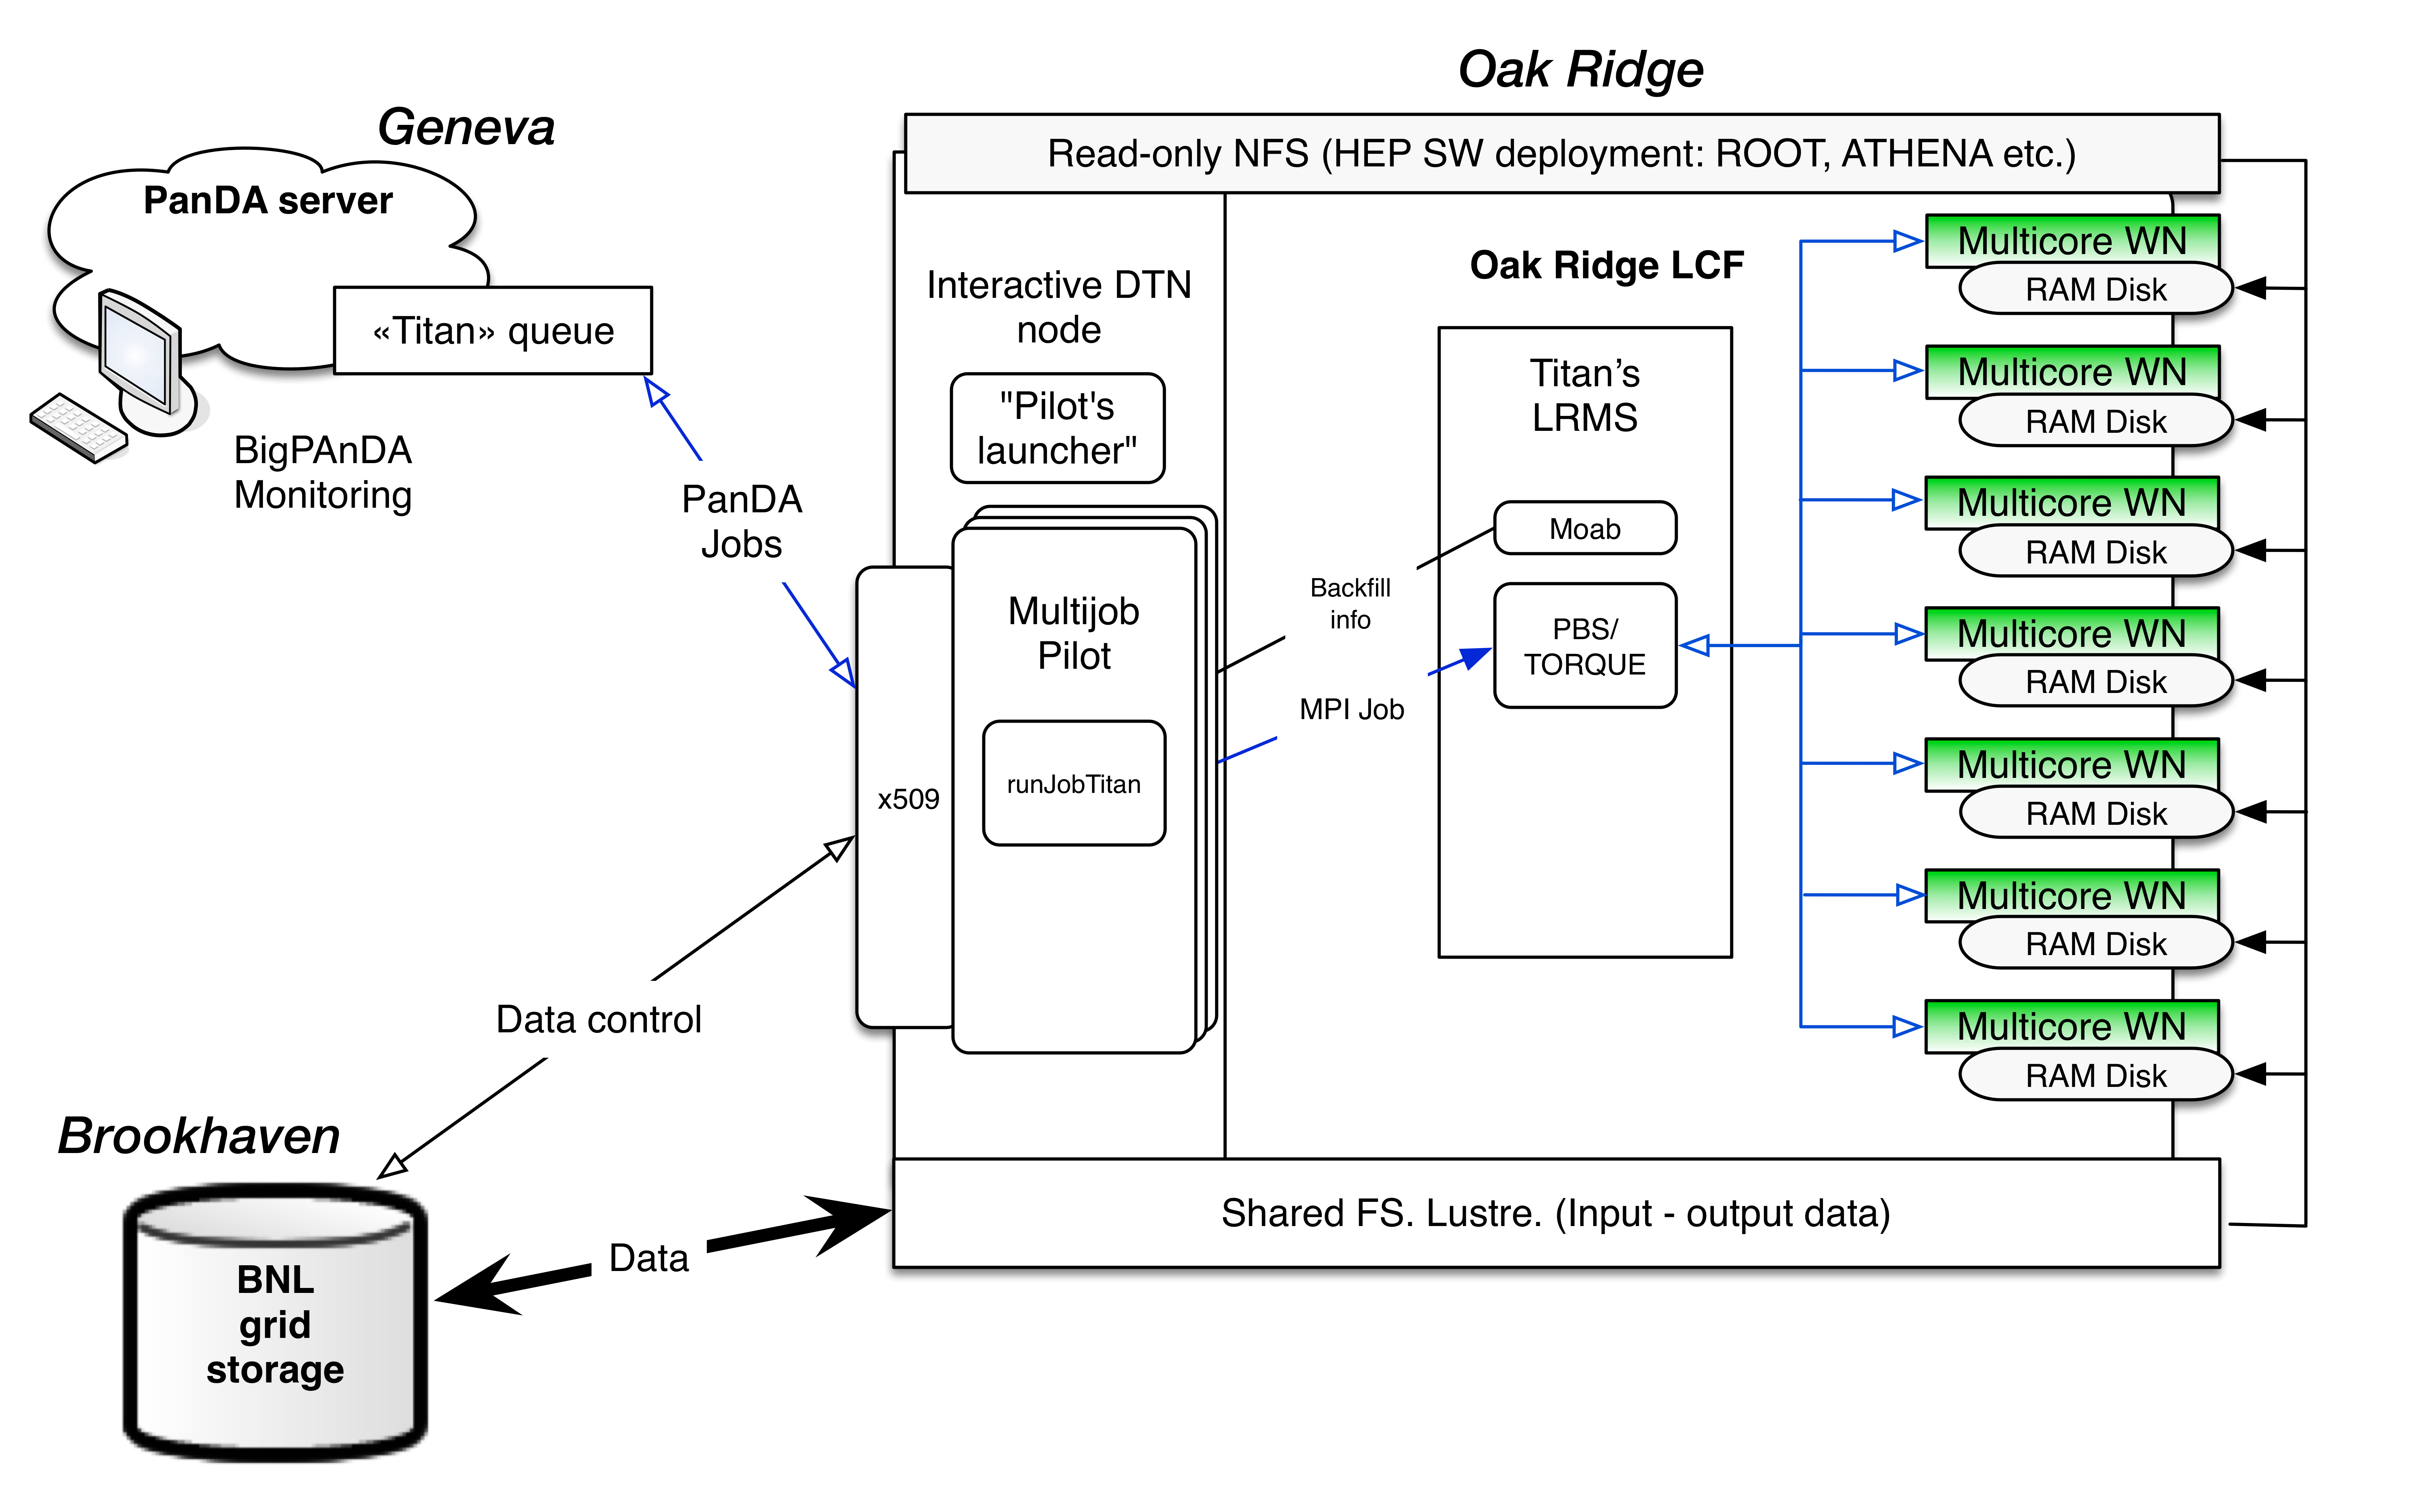
\includegraphics[width=0.75\textwidth]{images/Figure_5.png}
% figure caption is below the figure
\caption{Schematic view of PanDA WMS integration with Titan supercomputer at OLCF}
\label{fig:implementation}
\end{figure*}


% For two-column wide figures use
\begin{figure*}
% Use the relevant command to insert your figure file.
% For example, with the graphicx package use
  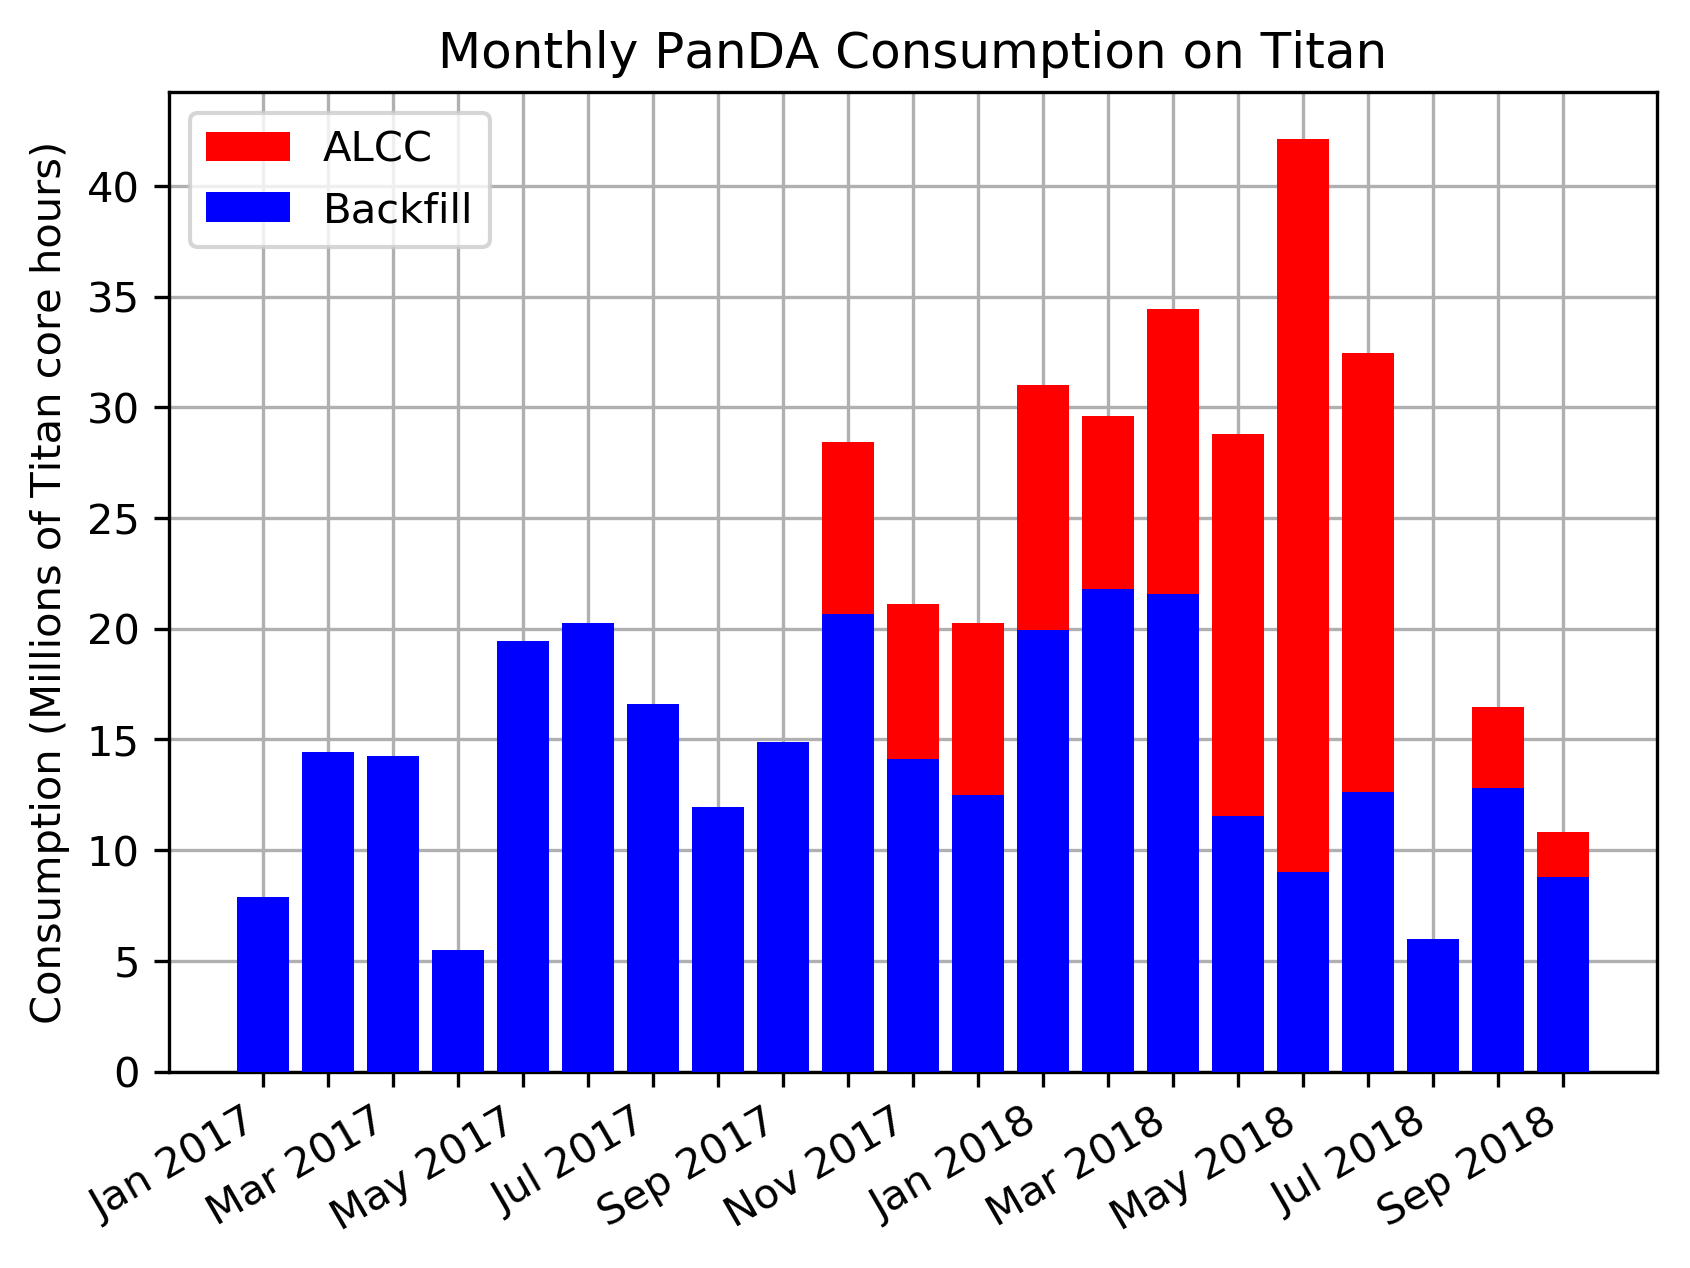
\includegraphics[width=0.75\textwidth]{images/monthly-consumption.png}
% figure caption is below the figure
\caption{This figure shows the monthly consumption of resources on Titan by the
two methods used by PanDA.}
\label{fig:monthly-consumption}
\end{figure*}

%-  vim:set syntax=tex:


% ---------------------------------------------------------------------------
% IV - Performance Characterization on Titan
% ---------------------------------------------------------------------------

\section{Impact Assessment of PanDA on Titan}
\label{sec:impact-assessment}
\jhanote{Performance of what? We should rename this section to some thing less
ambigious}
\seannote{Pretty much every section and subsection title can be tweaked, even
if only to make sure they all match the same parts of speech. I renamed it, but
obviously we can re-rename it.}

%-  LaTeX source file

%-  section4.tex ~~
%
%   This is the fourth section of the paper.
%
%                                                   ~~ last updated 22 Sep 2019

%%%%%%%%%%%%%%%%%%%%%%%%%%%%%%%%%%%%%%%%%%%%%%%%%%%%%%%%%%%%%%%%%%%%%%%%%%%%%%%

As outlined in Section~\ref{subsec:panda-at-olcf}, the BigPanDA team operated
under several OLCF project identifiers, including CSC108, a DD project which
sought to take advantage of ``backfill mode'' in order to consume unutilized
resources on Titan which would otherwise have gone to waste, without affecting
other projects' quality of service. The focus of this section is to assess the
degree to which CSC108 accomplished that goal and especially to analyze the
impact the project made on Titan.

\jhanote{there is a difference between ``idle'' and ``unutilized''. Need more
rigour in the definition of the stated goals}
\seannote{I admit I don't know the difference. What I generally intend is to
refer to machine which are available to perform work but aren't working.}
\jhanote{Idle is a state when not running. Underutilized is a ``response'' measured against a notion of adequate or desired utilization.}

% \jhanote{slightly misleading to claim there are three queues then to say
% immediately there is no backfill queue. Haven't we already discussed this in
% Section 3?}
% \seannote{It was confusing as written, so I moved the discussion of queues into
% Section 3.2. There was no backfill queue -- backfill was an optional feature
% that could be added to existing queues, and we played fast and loose in the
% past with how we referred to a ``queue'' that didn't actually exist.}

As a convention, we will sometimes make use of a common scheduling metaphor in
which jobs waiting to run on a computer are represented by rocks that are being
used to fill a jar. Capability class jobs on Titan are the largest rocks, and
the scheduler typically fills the remaining space around the largest rocks
with smaller rocks. CSC108 attempted to fill whatever space remains, thanks
to its having been given the lowest possible priority.

%%%%%%%%%%%%%%%%%%%%%%%%%%%%%%%%%%%%%%%%%%%%%%%%%%%%%%%%%%%%%%%%%%%%%%%%%%%%%%%%
\subsection{Rescheduling study}
\label{subsec:rescheduling-study}

% \jhanote{Please make the formulation of the statement more precise}
% \seannote{I'm not sure I made it any better, but I tried.} 

\jhanote{the following is a very strong statement. Discuss}

Recall that the goal of CSC108 was to consume unutilized resources on Titan
that would otherwise have remained unutilized, without decreasing the quality
of service experienced by other projects on Titan.  As shown in
Figure~\ref{fig:monthly-consumption}, CSC108 consumed hundreds of millions of
core hours on Titan. These resources are guaranteed to have been unutilized at
the time of that CSC108's jobs were scheduled because during that time period,
there was no pre-emption in the batch queue on Titan. Moreover, even if Moab
had ended running jobs in order to run other jobs with higher priorities
instead, CSC108's jobs would never have been used to replace existing jobs
because of the custom policies in place that guaranteed CSC108 would always
have the lowest priority on Titan. Therefore, CSC108 consumed millions of core
hours on Titan, all of which were guaranteed to have been unutilized at the
time that CSC108's jobs were scheduled.

It is a more difficult problem, however, to prove that these unutilized
resources on Titan would have remained unutilized and therefore ``gone to
waste''. For example, although the resources were unutilized at the time that
CSC108's jobs were scheduled, if other projects submitted jobs to Titan before
CSC108's jobs completed, then CSC108's jobs could be said to have ``blocked''
other jobs from running. This competition for resources would immediately imply
that, although some of the resources consumed by CSC108 would have gone to
waste, the rest of those resources would not have been wasted.

The simple bar plot shown in Figure~\ref{fig:jacks-slide} seems to show, at
first glance, that utilization by CSC108 has increased at the same time that
utilization by other projects has decreased, which is suggestive of competition
for resources. As a simple way to investigate this competition for resources,
we conducted an experiment in which three years' worth of job traces from Titan
were rescheduled, with and without CSC108's jobs, so that we could estimate
the impact of CSC108's jobs on wait times, throughput, and utilization for
Titan.

\jhanote{Hypothesis as currently formulated needs greater clarity: ``Has no
effect on Titan'' is too casual and clearly wrong, because it does increase
the utilization!} \seannote{I changed it to say ``null hypothesis''. It is
definitely a null hypothesis. The problem then, I suppose, is the implication
then that I will be seeking a p-value to test it.}

% \jhanote{Difficult to read /understand algorithm as is presented.}
% \seannote{I have updated to explain with more words and simpler pseudocode.}
% For two-column wide figures use
\begin{figure*}
% Use the relevant command to insert your figure file.
% For example, with the graphicx package use
  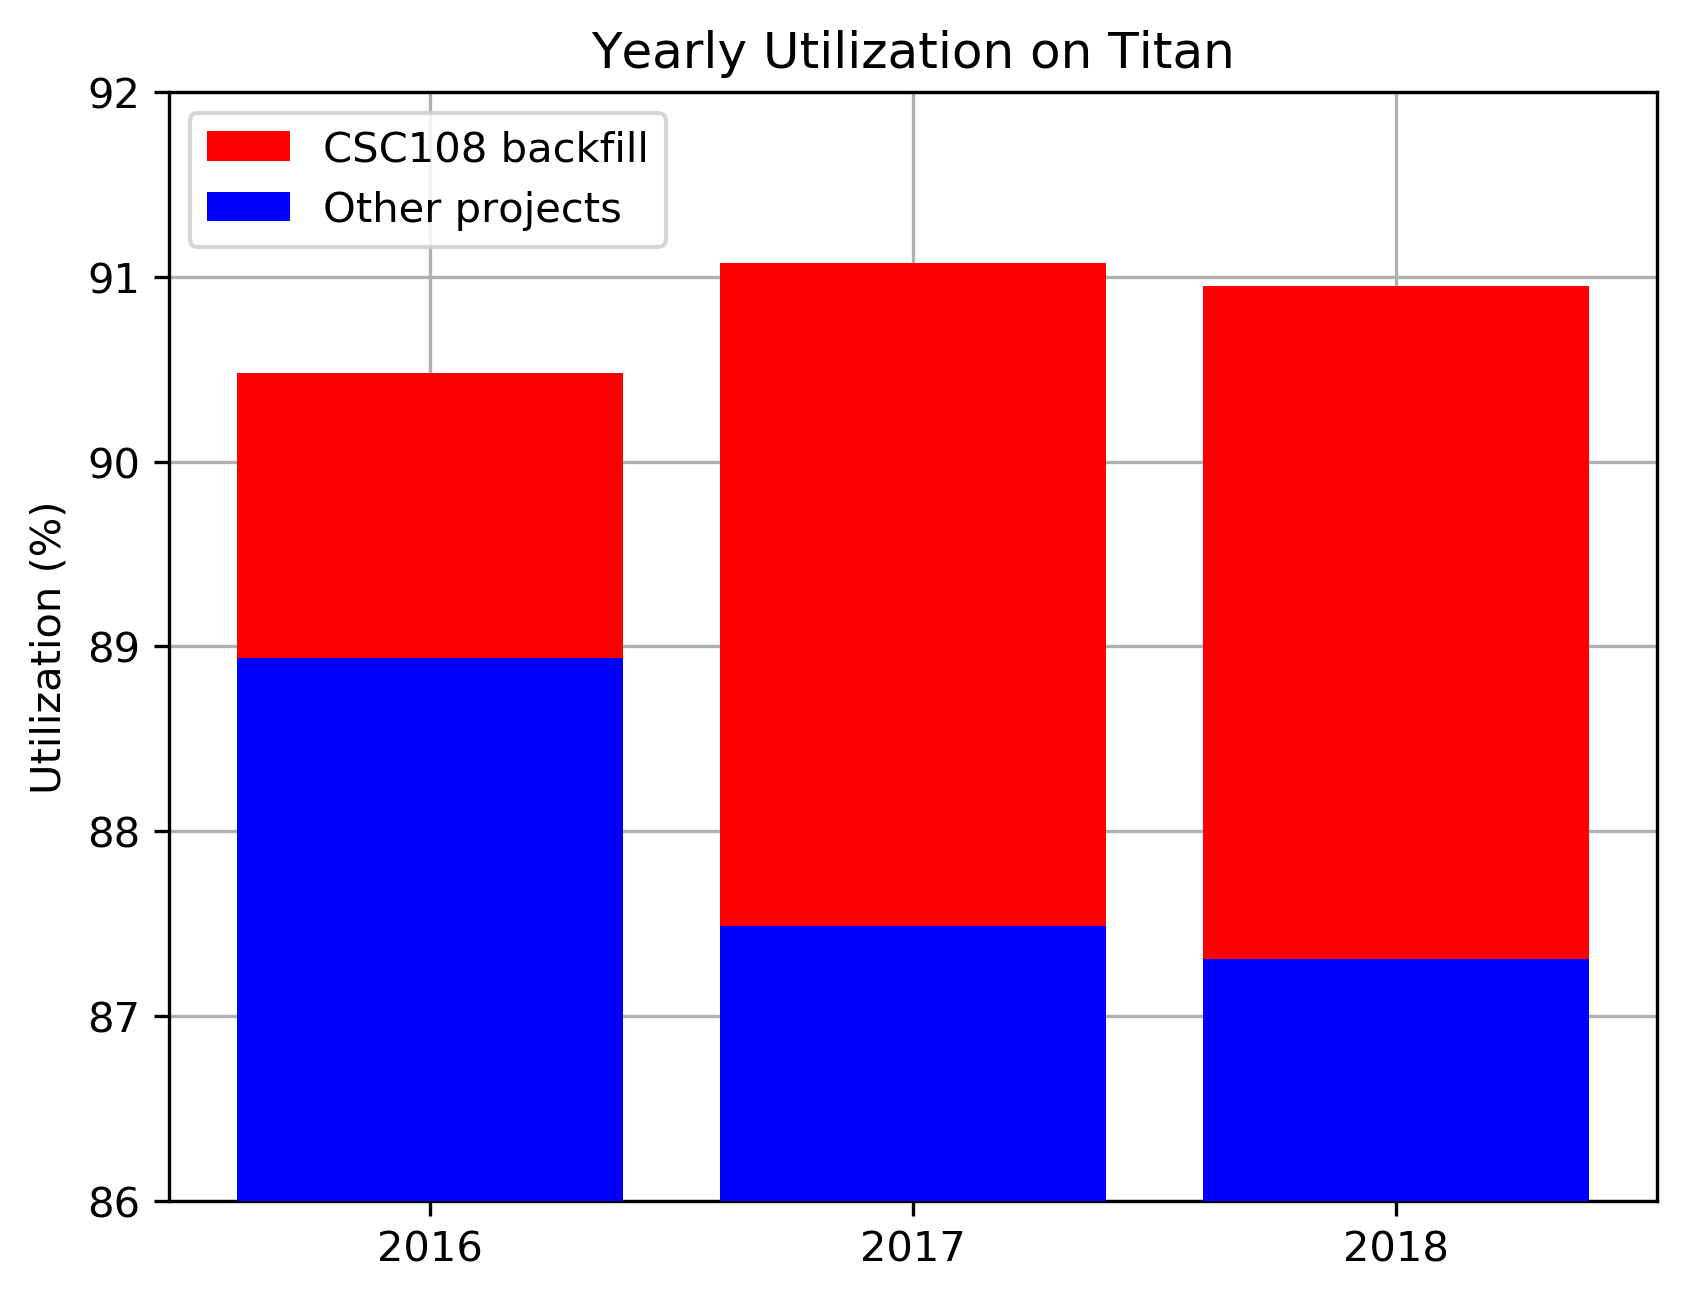
\includegraphics[width=0.75\textwidth]{images/barplot-jacks-slide.png}
% figure caption is below the figure
\caption{This bar plot visualizes the yearly utilization of Titan core hours,
separated into two categories: CSC108's utilization of Titan core hours through
backfill opportunities (shown in red), and all other utilization of core hours
on Titan (shown in blue).}
\label{fig:jacks-slide}
\end{figure*}

What we mean by ``compressing'' job traces is rescheduling the jobs that ran
on Titan while preserving the original execution order, under the assumption of
100\% node availability (all nodes up and running all the time). 

In order to reschedule the jobs, we made a simplifying assumption of 100\% node
availability, meaning that we assumed all of Titan's nodes were up and running
all the time. Original job execution order was also preserved. We rescheduled
the jobs once with CSC108's jobs included and then once with CSC108's jobs
removed, using the algorithm shown in Listing~\ref{lst:rescheduling.py} as
pseudo-code in the form of Python.

The idea here is akin to Archimedes's famous insight to measure the volume of
an irregularly shaped solid by measuring the difference in the volume of a
fluid before and after submerging the solid. In this case, however, we are
trying to evaluate the fluid, because we are most interested in the fluid's
ability to fill the irregular ``spaces'' between the other projects' jobs. The
difference in the completion times for the last scheduled job, with and without
CSC108, provide insight about the ability of CSC108's jobs to fit precisely
in the spaces between other jobs. This rescheduling technique also allows
CSC108's jobs' effects on throughput and utilization to be estimated in a
simple way, by simply computing them with and without CSC108's jobs included
with the other job traces. Throughput was defined as jobs completed per day,
and utilization was defined as the percentage of available core hours which
were consumed.

The data used for this experiment are historical traces for all jobs on Titan
during the years 2016, 2017, and 2018. These data were provided in anonymized
form by OLCF so that job, project, and user identifiers were included only for
the three PanDA projects on Titan. Otherwise, the job traces consist only of
job submission time, start time, completion time, the number of requested
nodes, and the amount of wall time requested. The experimental programs were
written in Python using the well-known Matplotlib, NumPy, and SciPy libraries
via Anaconda. Data were originally provided as text files but were imported
into a SQLite database.

\lstinputlisting[language=Python,
    label={lst:rescheduling.py},
    caption={Job traces are assumed to be sorted in order of original start
                time.}]{rescheduling.py}

The results, which are summarized in Table~\ref{tab:rescheduling-results}, show
that including CSC108's jobs when rescheduling results in the simulation taking
13.3 additional days of simulation time, which represents a 1.30\% increase in
the total time to completion. Throughput increases by 190.26 jobs per day,
which represents a 14.36\% increase, and utilization increases from 92.36\% to
94.15\%, which is a 1.94\% increase when CSC108's jobs are included versus when
they are omitted.

If CSC108's jobs fit perfectly within the spaces between the other projects'
jobs, then we would expect there to be no difference between the simulation's
times to completion with and without CSC108's jobs. The simulation observed a
1.30\% increase in time to completion, however, which indicates that CSC108's
jobs did not fit perfectly within the spaces in the simulation, and this
suggests that CSC108's jobs do not fit perfectly within the spaces in real
life. This also serves as an estimate for the impact of CSC108's jobs on the
wait times experienced by other projects' jobs on Titan, because an increase of
1.30\% over a three-year period represents an average of sorts for shorter
time periods. This result suggests that CSC108's jobs may impact other jobs on
Titan by increasing their wait times.

If CSC108's jobs fit perfectly within the spaces between other projects' jobs,
then we would expect to observe an increase in throughput, which is defined
here as jobs completed per day, because every CSC108 job that completed would
represent one more job that would not have completed if CSC108's jobs had been
removed. The simulation observed a 14.36\% increase to throughput, but this
number is ambiguous when evaluated on its own. For example, the same number of
Titan core hours can be consumed as one large job or a large number of small
jobs, but in the latter case, throughput may be considerably higher.

Finally, if CSC108's jobs fit perfectly within the spaces between the other
projects' jobs, then we would expect to observe an increase in utilization,
because all utilization by CSC108's jobs would represent utilization of
resources which would otherwise have remained unutilized. The simulation
observed a 1.94\% increase in utilization, but like throughput, this number is
also ambiguous when evaluated on its own. For example, an increase in
utilization could also occur in a scenario where CSC108 was using 100\% of
Titan, causing all other projects to wait.

The results in Table~\ref{tab:rescheduling-results} do imply, however, that
some of the resources consumed by CSC108's jobs in the simulation would have
gone to waste. This is because the product of the time to completion and the
utilization can be used to calculate the total amount of resources consumed
during each simulation run. Without CSC108's jobs included, the remaining jobs
required 1021.2 days of simulation time on Titan to complete, and they consumed
92.36\% of Titan's resources during that time; this is an equivalent amount of
work, when redistributed, to consuming 943.18 days of 100\% of Titan's
resources. By a similar calculation, 973.98 Titan-days of computation were
consumed when CSC108's jobs were included, and this implies that CSC108's jobs
were responsible for 30.8 Titan-days of resource consumption. Because the two
runs' times to completion differed by only 13.3 days, it is impossible for
CSC108 not to have used at least some of the resources which would have gone to
waste.

So, while it is difficult to label exactly which resources would have gone to
waste and when, the simulation results suggest that some non-zero portion of
the resources consumed by CSC108 would have gone to waste. The simulation
results also indicated that CSC108's jobs did not fit perfectly within the
spaces between the other projects' jobs, which suggests that CSC108 ``blocks''
other projects some of the time and that some non-zero portion of the resources
consumed by CSC108 would not have gone to waste.

\jhanote{Need more set-up: why do we choose these three metrics? Define them in text too? Contextualize 1.3\% (collective) versus fluctuation per individual
jobs in queue. Once again, the following claim / statement is wrong: ``''must
have consumed resources which would otherwise have gone to waste.``. Recall
the statement ``must have consumed resources which would otherwise have gone
to waste.`` is a corollary to the hypothesis that ``CSC108 does not impact
Titan''... so you cannot use that to justify the hypothesis.}
\seannote{I killed off the use of language related to a ``hypothesis'' to try
to clean things up, and I used a new data-based argument for why the simulation
suggests that CSC108 partially uses resources which would otherwise have gone
to waste.}

% For tables use
\begin{table}
% table caption is above the table
\caption{Rescheduling study results}
\label{tab:rescheduling-results}       % Give a unique label
% For LaTeX tables use
\begin{tabular}{lrrr}
\hline\noalign{\smallskip}
\phantom{booga}     &   Without CSC108  &   With CSC108 &   Percent change  \\
\hline\noalign{\smallskip}
Time to completion (days)           &   1021.2  &   1034.5  &   1.30        \\
Throughput (jobs per day)           &   1324.93 &   1515.19 &   14.36       \\
Utilization (percent)               &   92.36   &   94.15   &   1.94        \\
\noalign{\smallskip}\hline
\end{tabular}
\end{table}


%%%%%%%%%%%%%%%%%%%%%%%%%%%%%%%%%%%%%%%%%%%%%%%%%%%%%%%%%%%%%%%%%%%%%%%%%%%%%%%%
\subsection{Searching for simple linear relationships}
\label{subsec:simple-linear-relationships}

\jhanote{relationships of what to what? is the result being used as the
subsection title?}
\seannote{I don't know what to call it. I looked across dozens of combinations
of variables with ordinary least squares regression and never found anything
conclusive. I had to give it a title of some kind. Naming is hard.}

% \jhanote{Please be specific about the ecosystem, viz., the QOS for other users
% as measured by their average wait time.} \jhanote{of what??} \jhanote{unclear opening. I think it needs rewrite.} \seannote{I rewrote it. It sounds similar but
% it has more details \ldots ?}

Recall that the goal of CSC108 was to consume resources on Titan which would
otherwise have gone unutilized, while not decreasing the quality of service for
other projects on Titan. The results of Section~\ref{subsec:rescheduling-study}
suggested that CSC108 consumed resources which might have gone to waste, but
that it also may have impacted other projects' quality of service. This section
details further explorations to understand the impact of CSC108 on Titan by
searching for simple linear relationships, especially direct and inverse
relationships, between variables like bin size and indicators like wait times,
throughput, and utilization, by using ordinary least-squares regression.

The data used for this experiment include the same historical trace data used
in Section~\ref{subsec:rescheduling-study}, supplemented with daily availability
data for Titan provided by OLCF for the same years, 2016-2018. The experimental
programs were written in Python using the well-known Matplotlib, NumPy, SciPy,
and scikit-learn libraries via Anaconda. Data were originally provided as text
files but were imported into a SQLite database. We plotted best-fit lines with
ordinary least squares (OLS) linear regression, constructed 95\% confidence
regions around the lines, and used basic measures for goodness-of-fit such as
R-squared.

There were two main ideas used here. The first idea was to look for a
relationship between CSC108's throughput and the throughput of all other jobs
on Titan, and second idea was to look for a relationship between CSC108's
utilization as compared with overall utilization on Titan. Additionally, the
same ideas were repeated to look for impacts due to different sizes of CSC108's
jobs, using the bins defined in Table~\ref{tab:olcf-bins}, because jobs are
assigned priority differently by the scheduler on Titan in part due to the
number of requested nodes and length of requested wall time.

%%%
% THROUGHPUT FIGURES AS SUBFIGURES
%%%
\begin{figure*}
  \subfloat[All\label{fig:throughput-all}]{
    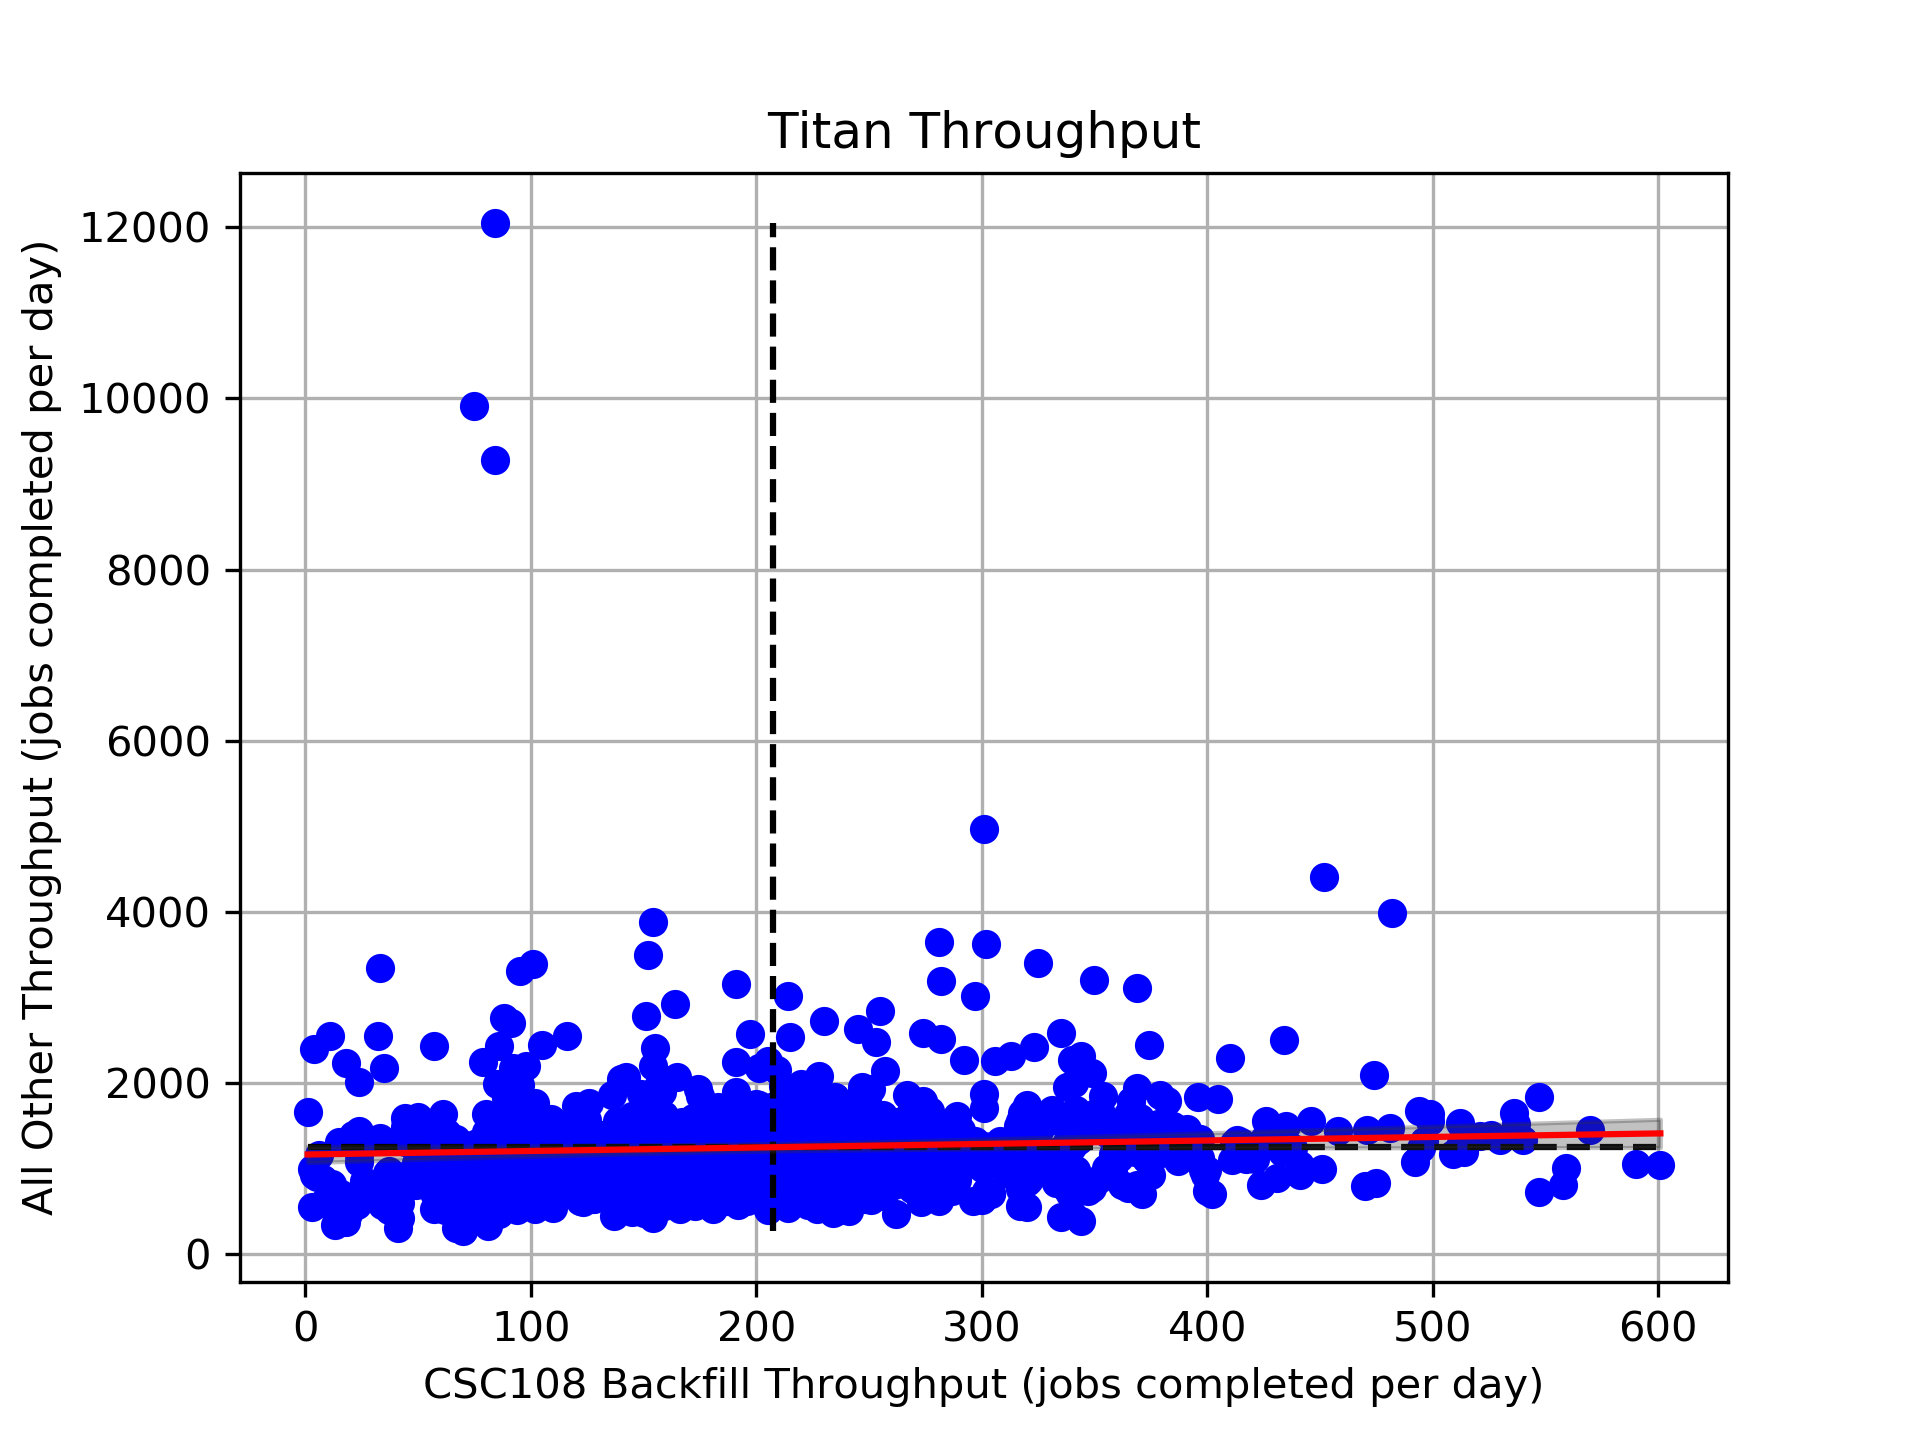
\includegraphics[width=0.4\textwidth]{images/linfit-throughput-all.png}}
  \subfloat[Bin 3\label{fig:throughput-bin3}]{
    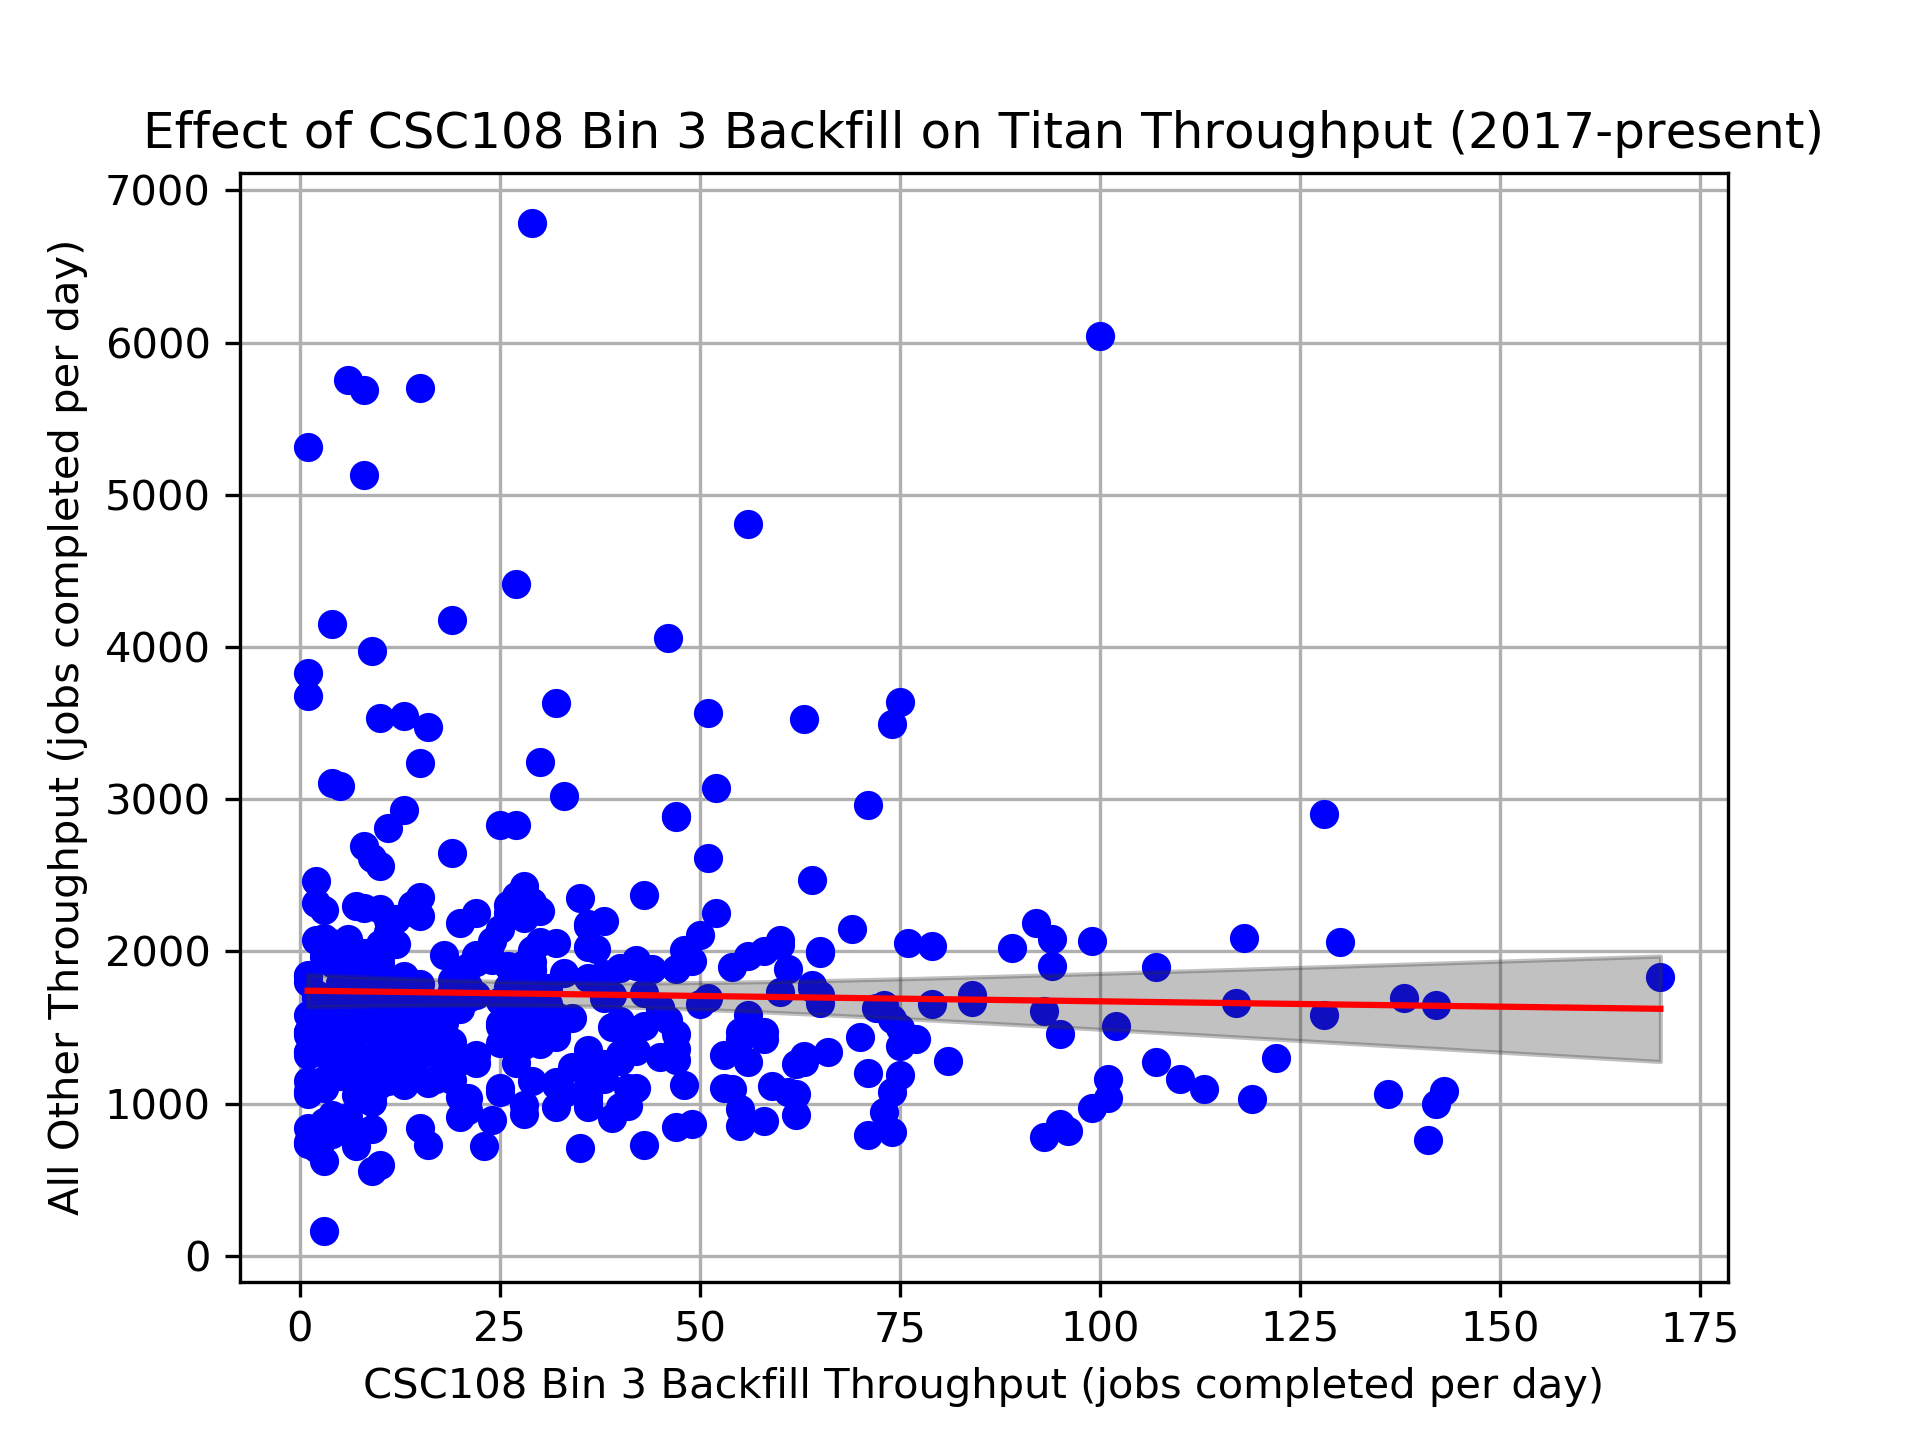
\includegraphics[width=0.4\textwidth]{images/linfit-throughput-bin3.png}}
  \vspace{1em}
  \subfloat[Bin 4\label{fig:throughput-bin4}]{
    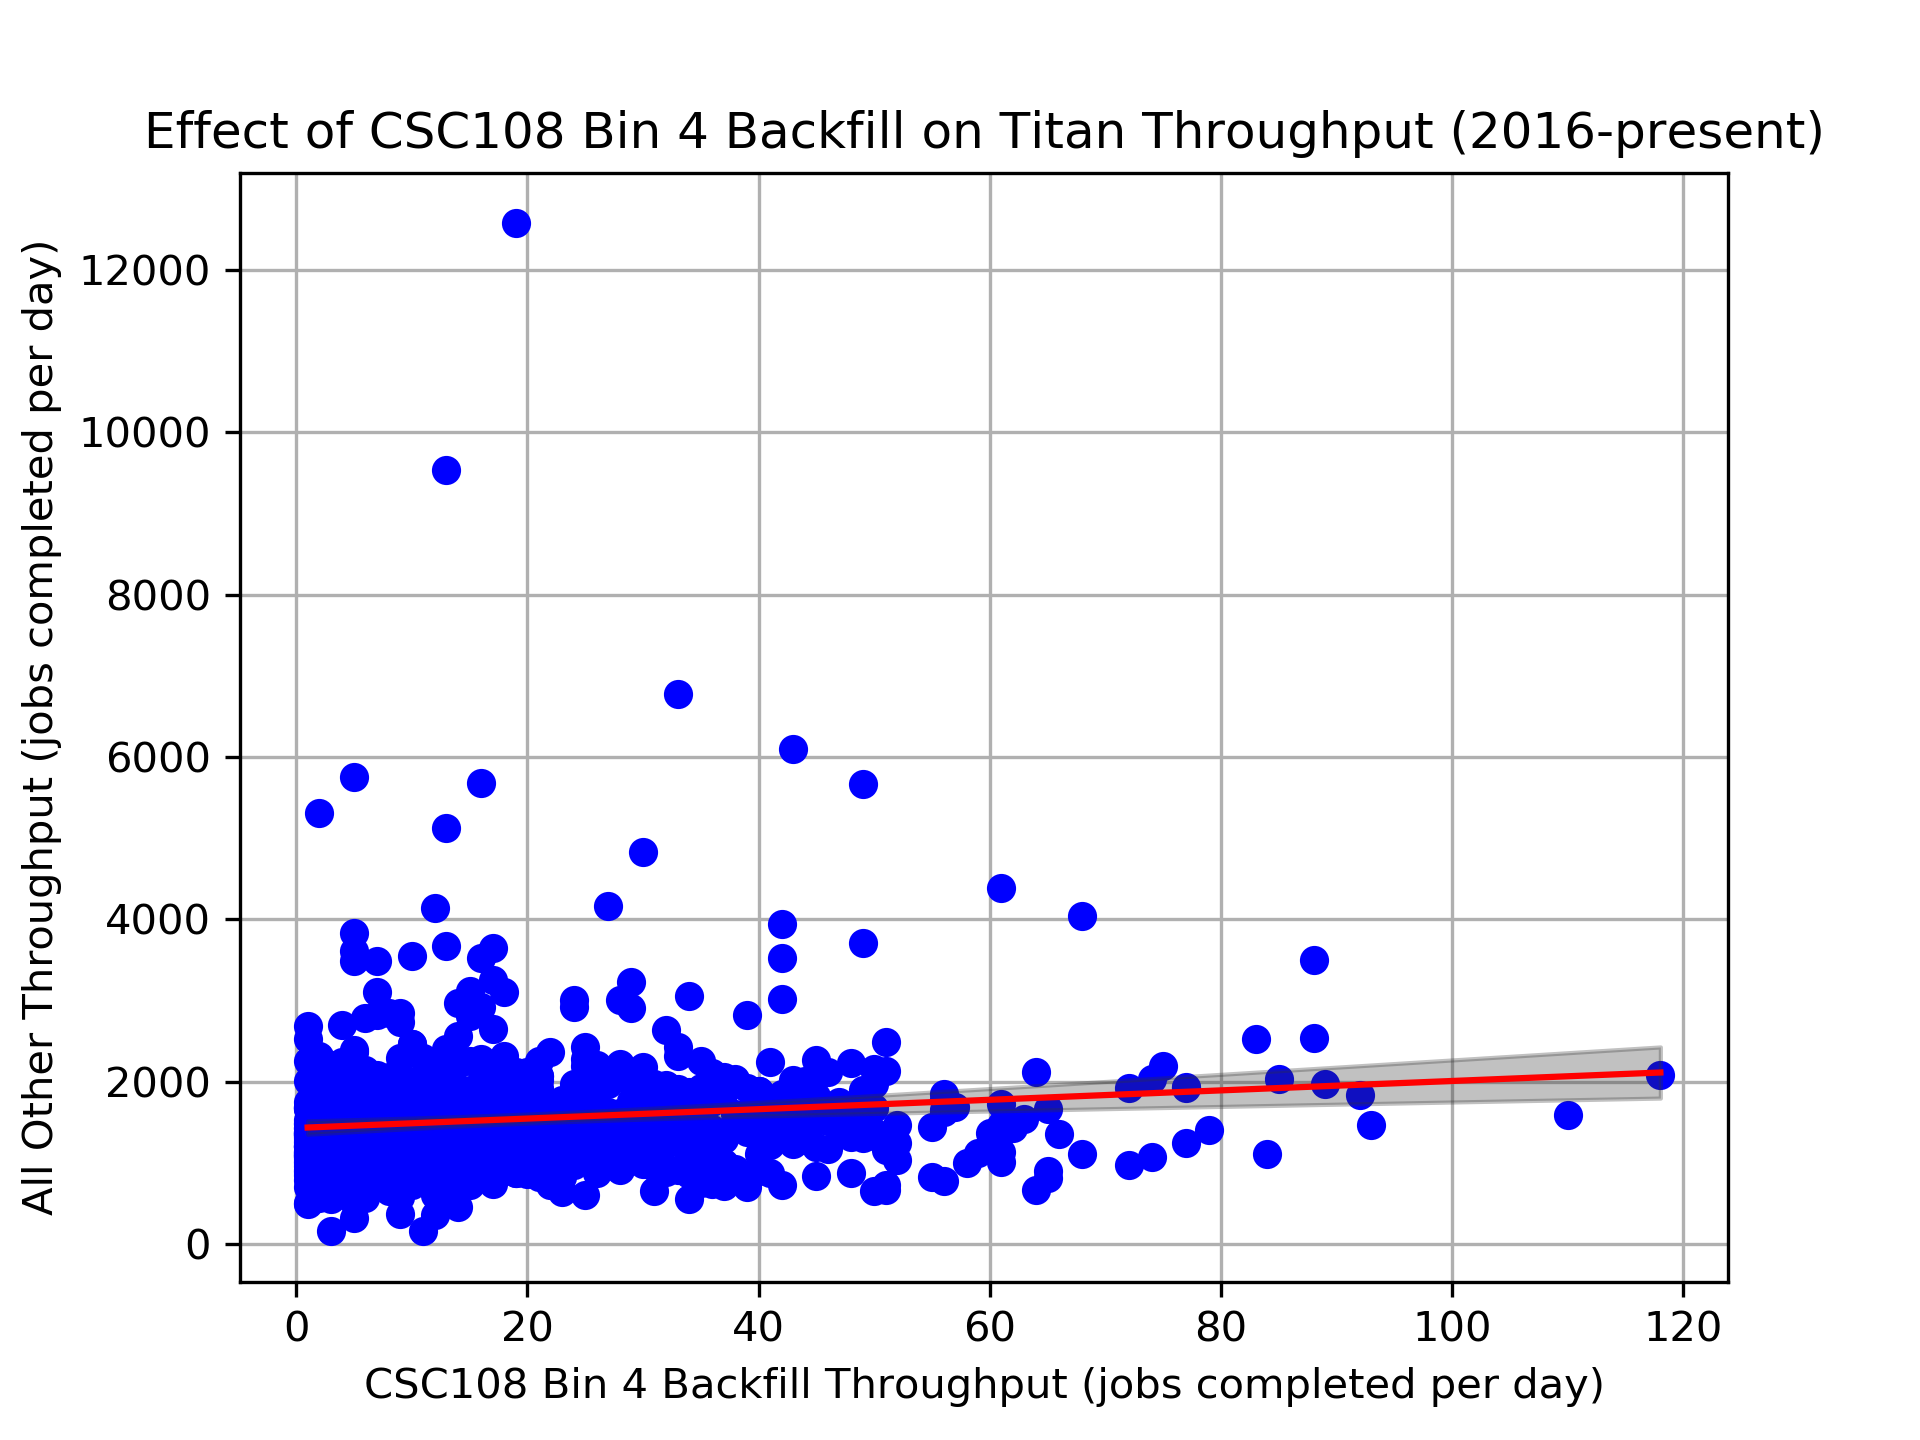
\includegraphics[width=0.4\textwidth]{images/linfit-throughput-bin4.png}}
  \subfloat[Bin 5\label{fig:throughput-bin5}]{
    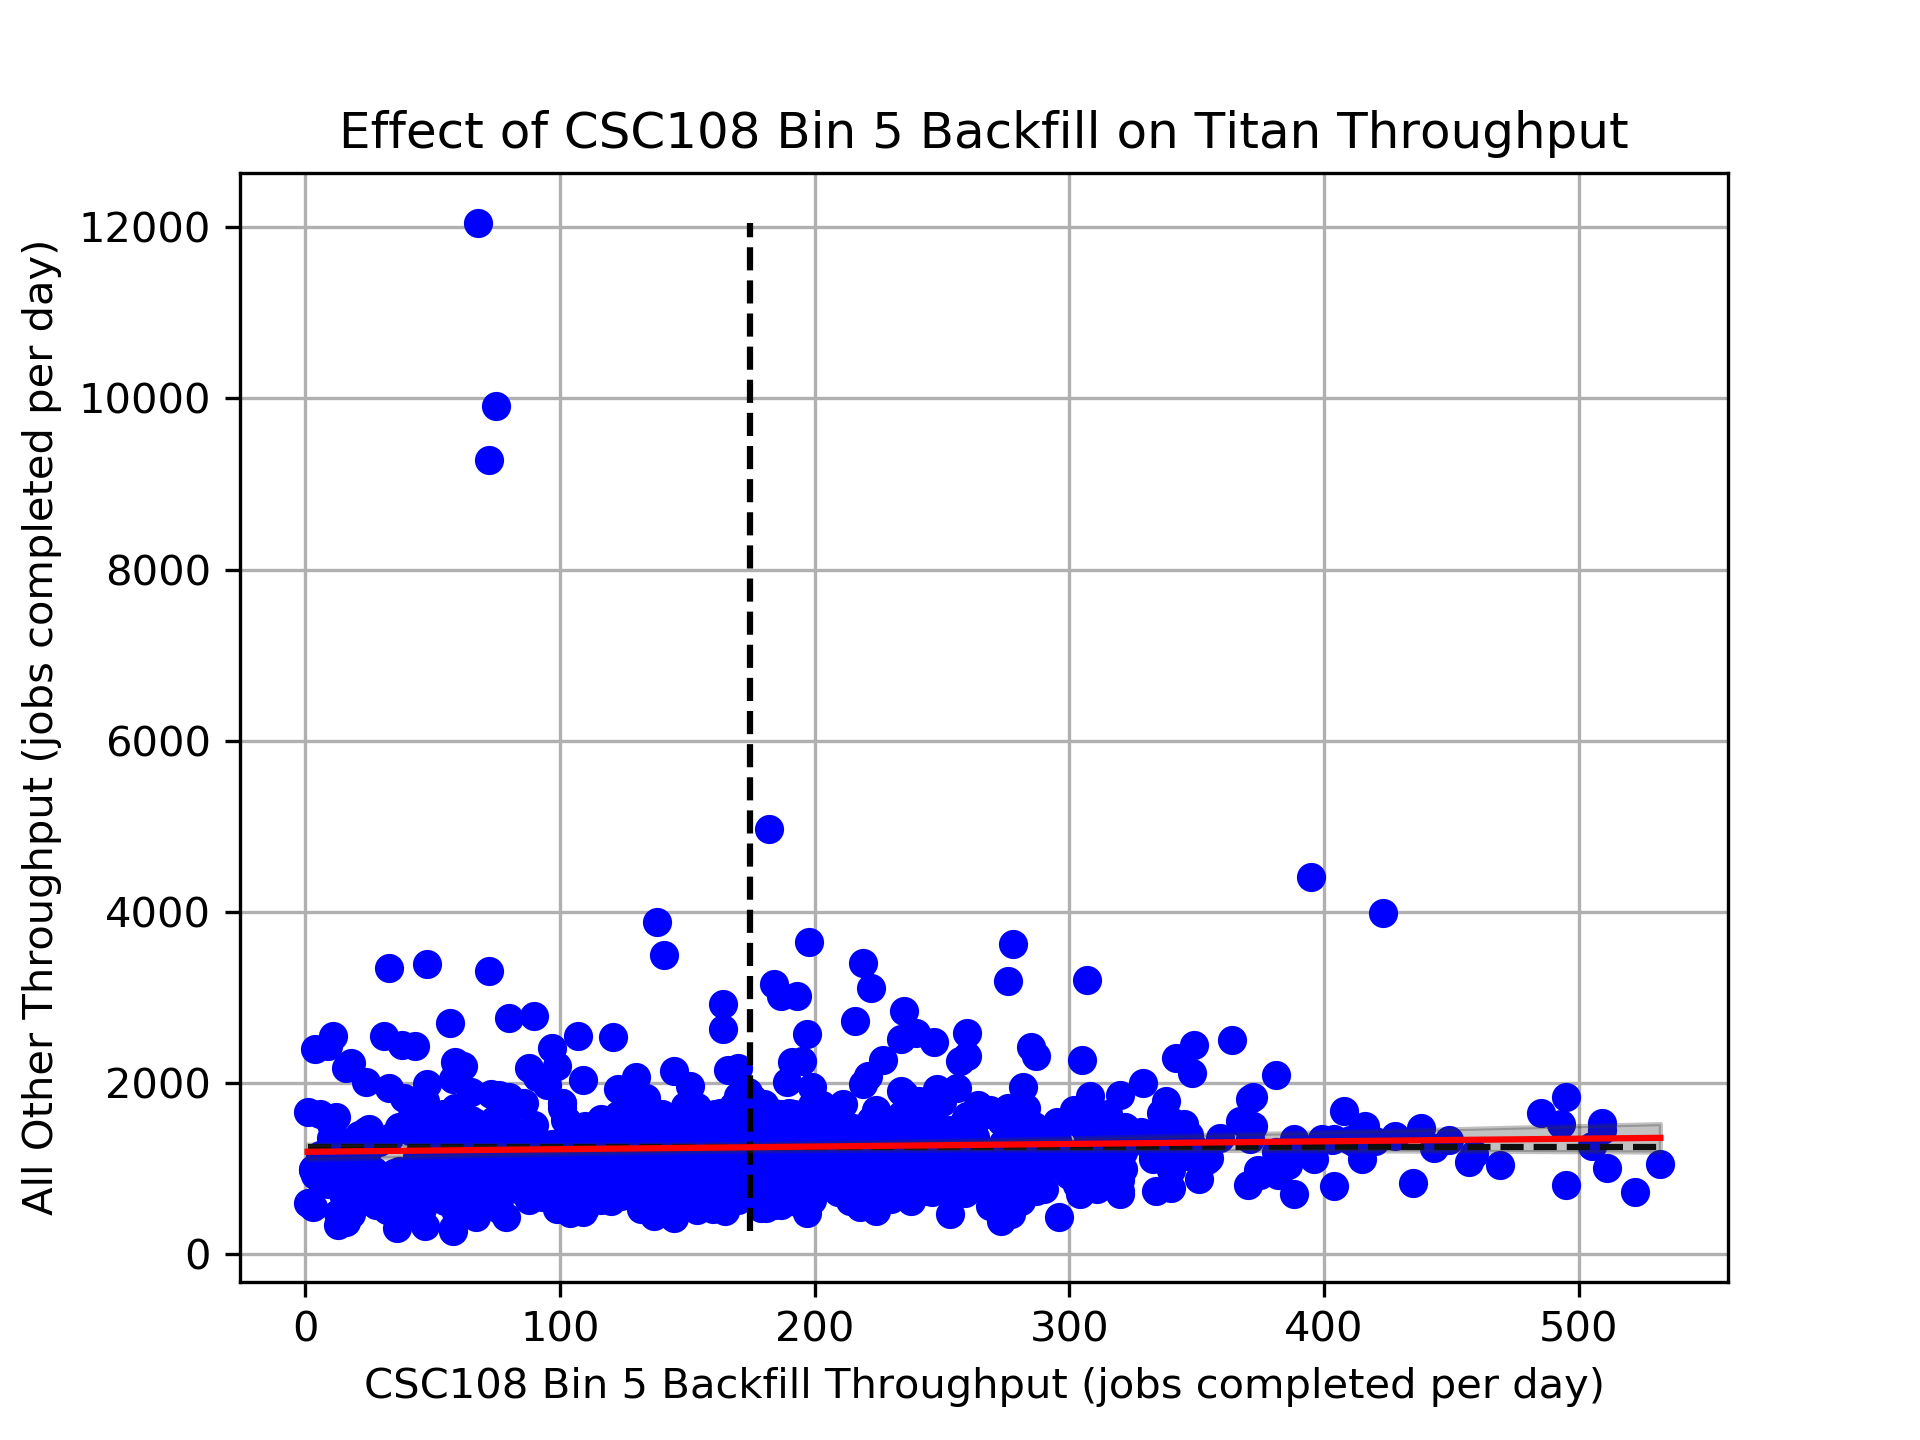
\includegraphics[width=0.4\textwidth]{images/linfit-throughput-bin5.png}}
  \caption{This figure demonstrates the relationship between CSC108 backfill
throughput and throughput of other projects on Titan, in terms of jobs
completed per day. Each blue point represents one day. Each red line is an
Ordinary Least Squares (OLS) linear regression with parameters given in
Table~\ref{tab:throughput-params}. Each shaded gray area represents a 95\%
confidence region. Each horizontal dotted black line represents the mean number
of jobs completed on Titan every day by projects other than CSC108, and the
vertical dotted black line represents the mean number of jobs completed every
day by CSC108's use of backfill opportunity.}
\end{figure*}

% For tables use
\begin{table}
% table caption is above the table
\caption{The table contains the parameter values for the Ordinary Least Squares
(OLS) linear regression models regarding throughput. The first column
corresponds to the figure depicting the model, and the second column
corresponds to the OLCF bin number, as defined in Table~\ref{tab:olcf-bins}.
The second and third columns correspond the coefficients $\beta_1$ and
$\beta_0$ in the model $y = \beta_{1}x + \beta_0$.}
\label{tab:throughput-params}       % Give a unique label
% For LaTeX tables use
\begin{tabular}{ccrrr}
\hline\noalign{\smallskip}
Figure & OLCF Bin & Slope $\beta_1$  & Intercept $\beta_0$  &   $\text{R}^2$ \\
\noalign{\smallskip}\hline\noalign{\smallskip}
\ref{fig:throughput-all}    &   All &   0.4106  &   1164.2561   & 0.0040    \\
\ref{fig:throughput-bin3}   &   3   &   0.4419  &   1322.0784   & 0.0005    \\
\ref{fig:throughput-bin4}   &   4   &   1.9819  &   1211.3384   & 0.0027    \\
\ref{fig:throughput-bin5}   &   5   &   0.3072  &   1195.6684   & 0.0018    \\
\noalign{\smallskip}\hline
\end{tabular}
\end{table}
%%%

%%%
% UTILIZATION FIGURES AS SUBFIGURES
%%%
\begin{figure*}
  \subfloat[All\label{fig:utilization-all}]{
    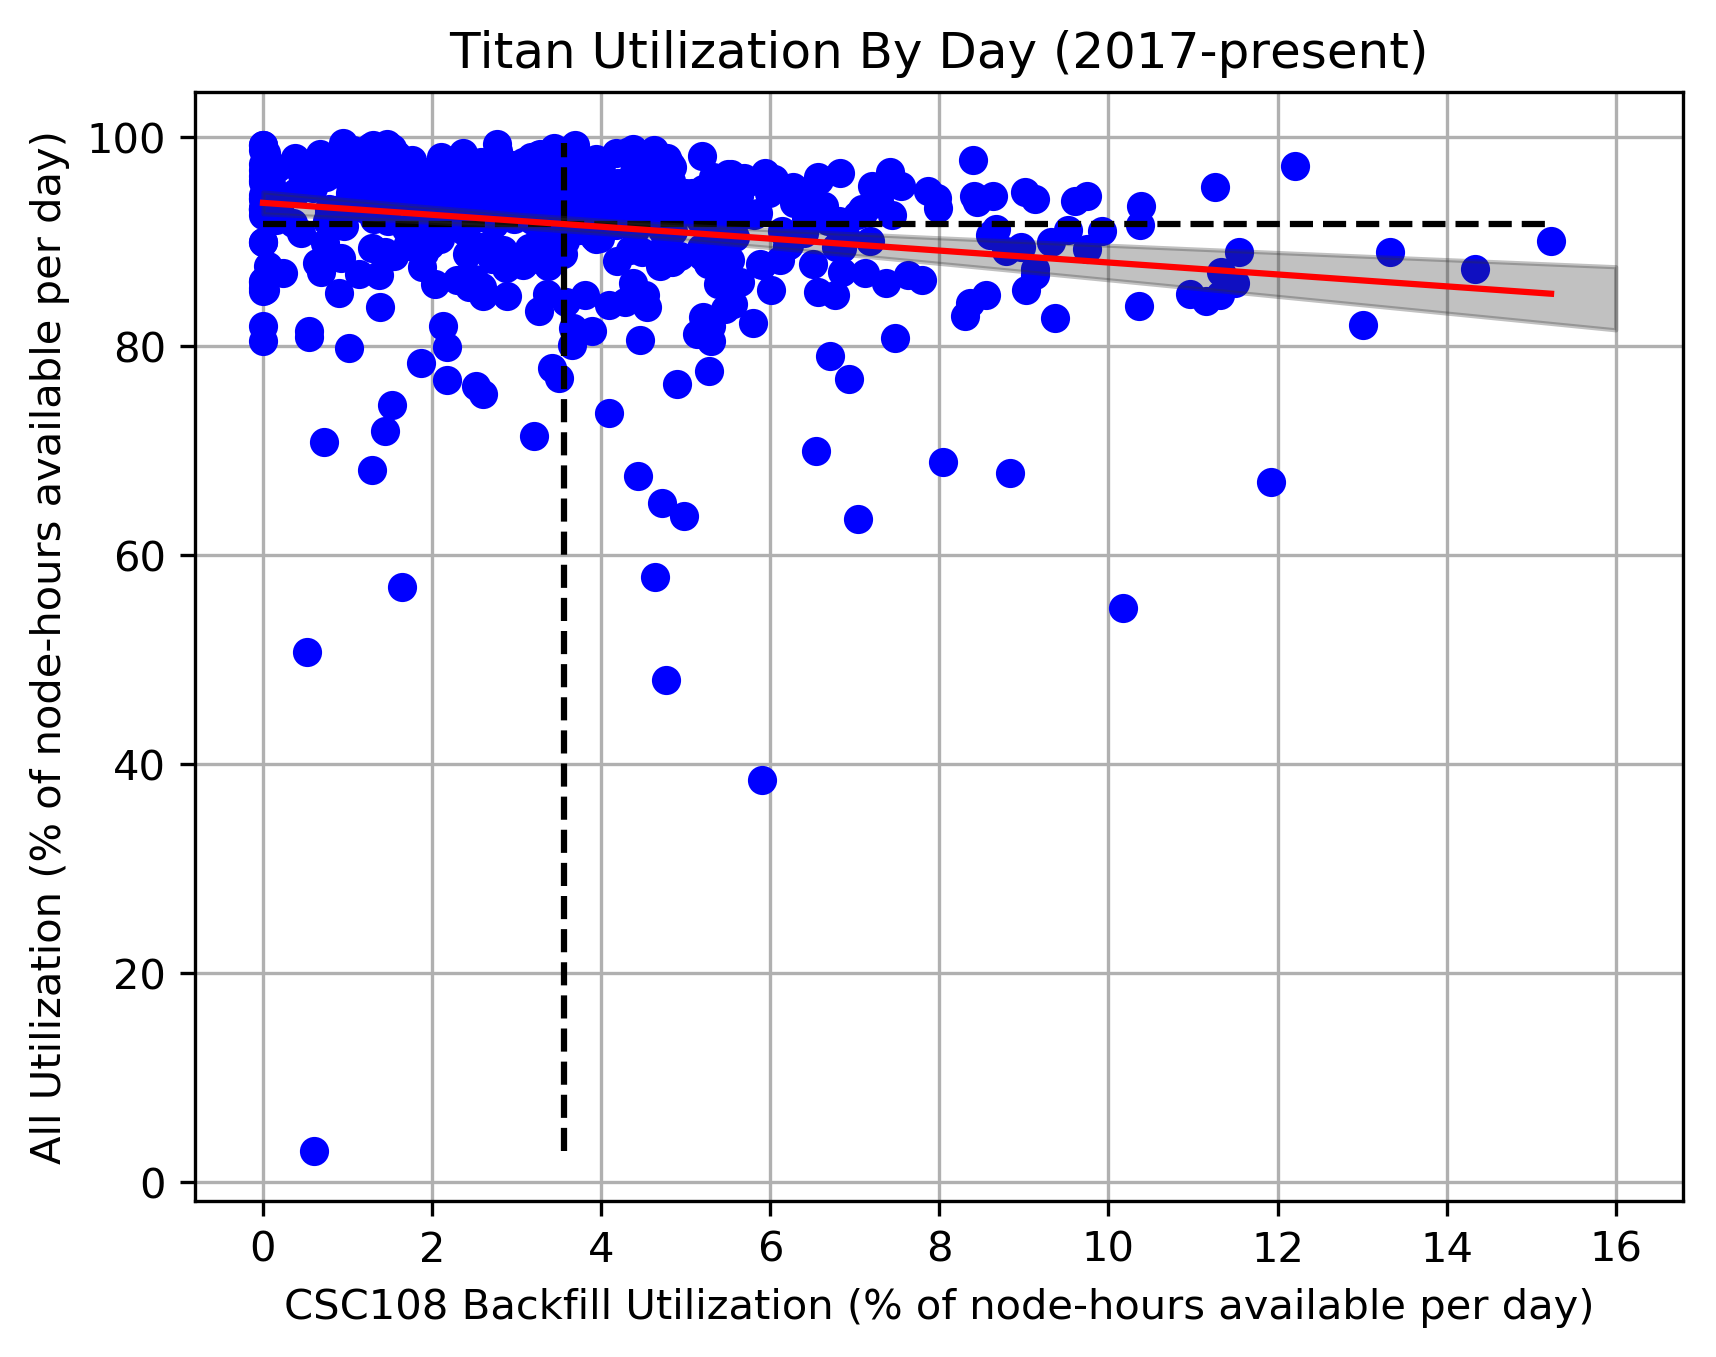
\includegraphics[width=0.4\textwidth]{images/linfit-utilization-by-true-day-all.png}}
  \subfloat[Bin 3\label{fig:utilization-bin3}]{
    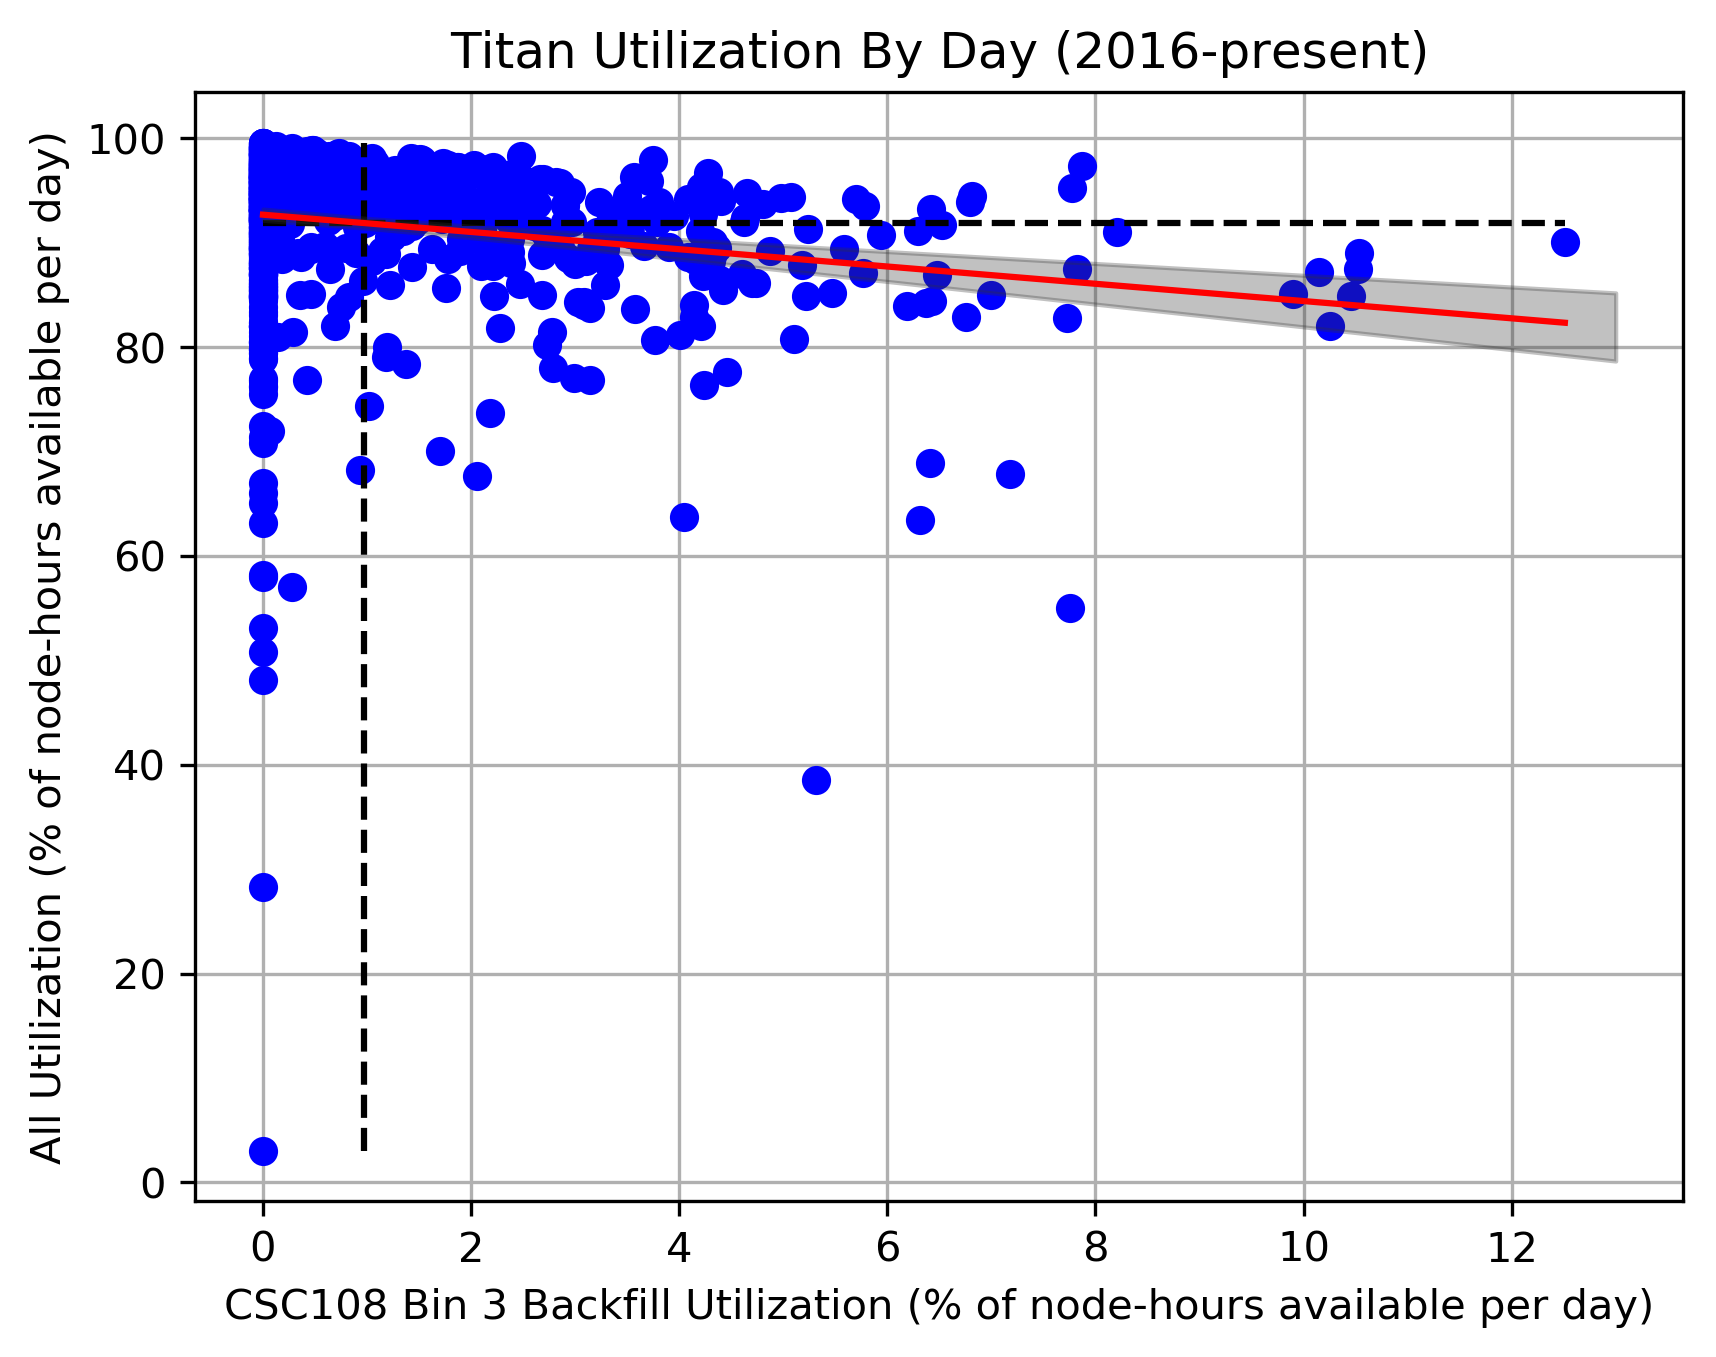
\includegraphics[width=0.4\textwidth]{images/linfit-utilization-by-true-day-bin3.png}}
  \vspace{1em}
  \subfloat[Bin 4\label{fig:utilization-bin4}]{
    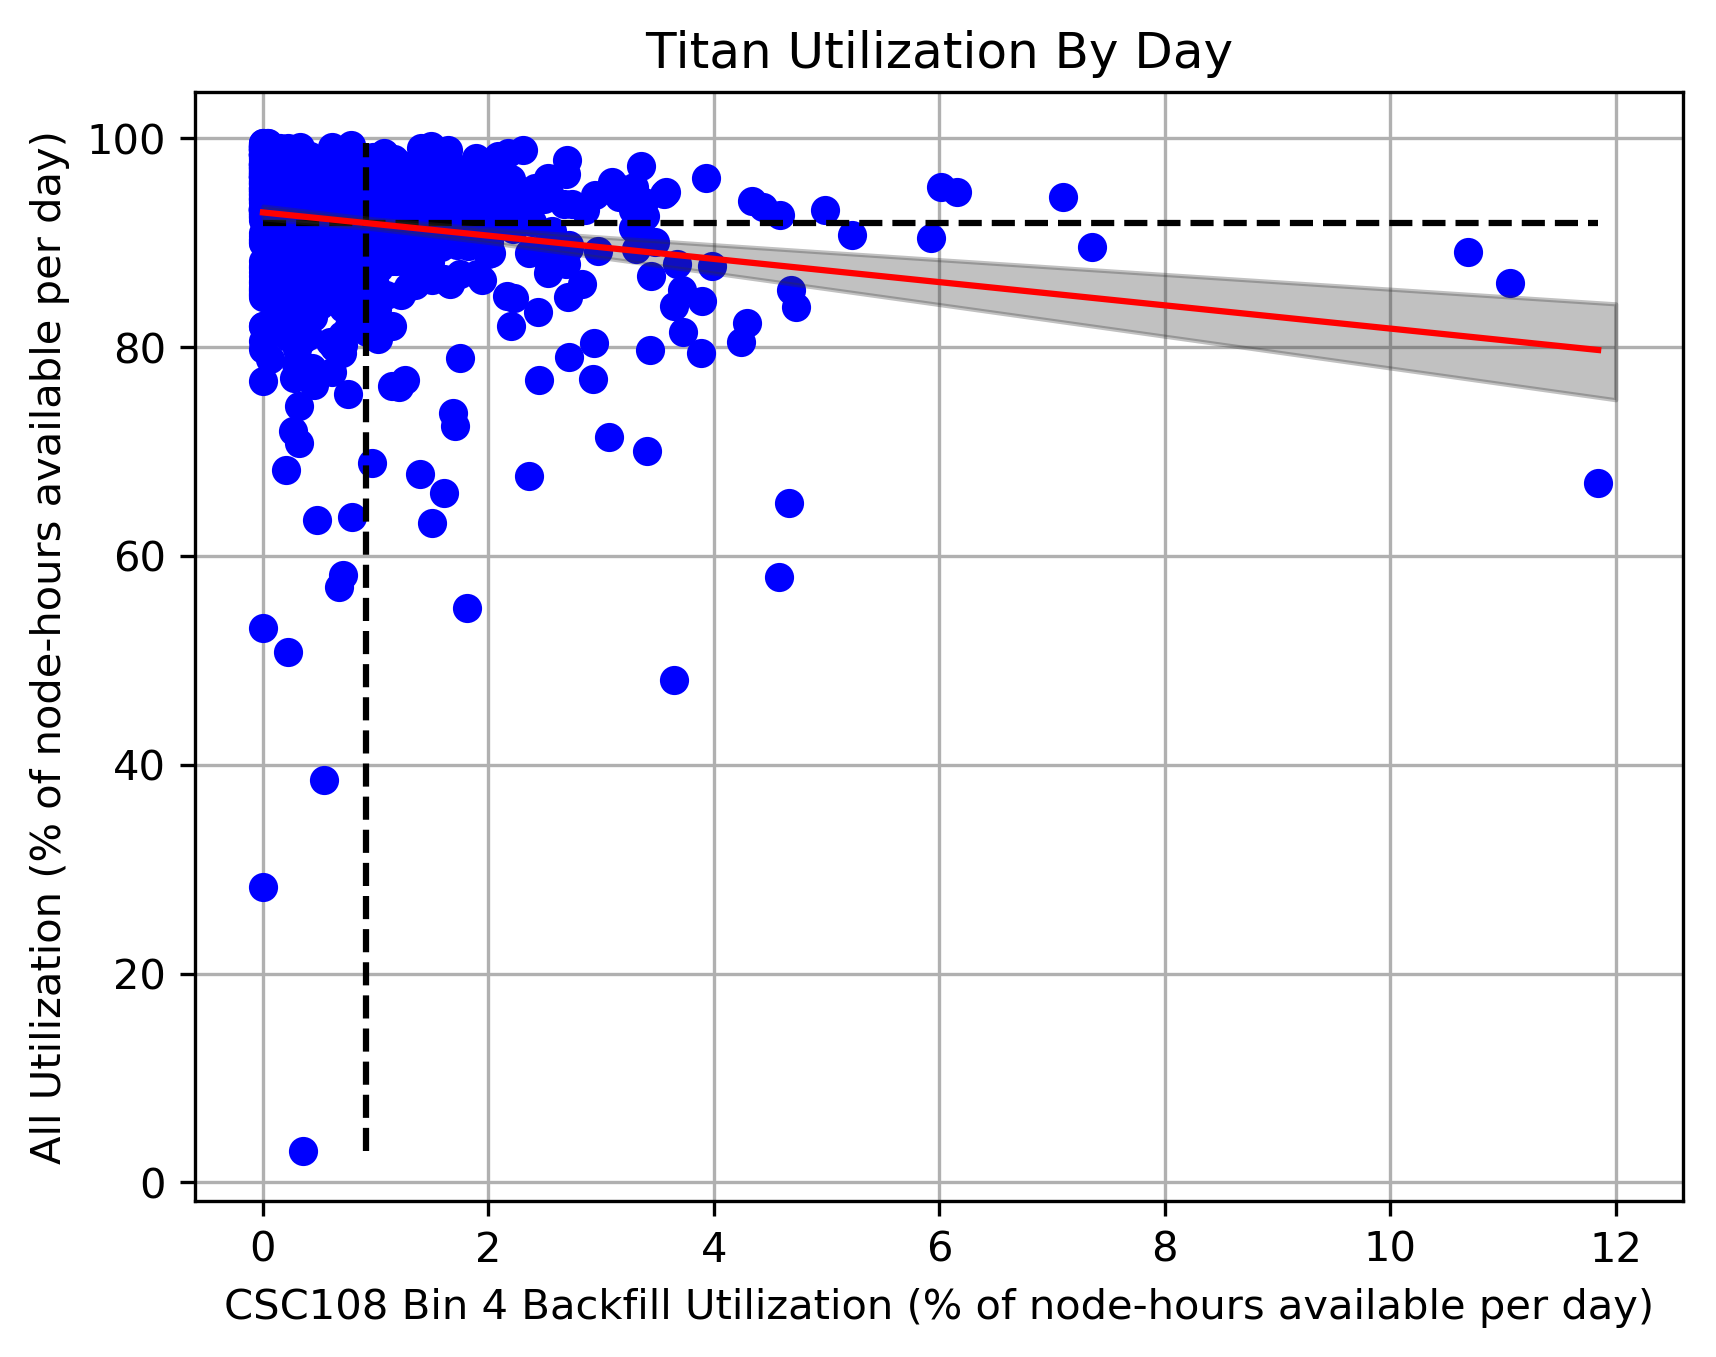
\includegraphics[width=0.4\textwidth]{images/linfit-utilization-by-true-day-bin4.png}}
  \subfloat[Bin 5\label{fig:utilization-bin5}]{
    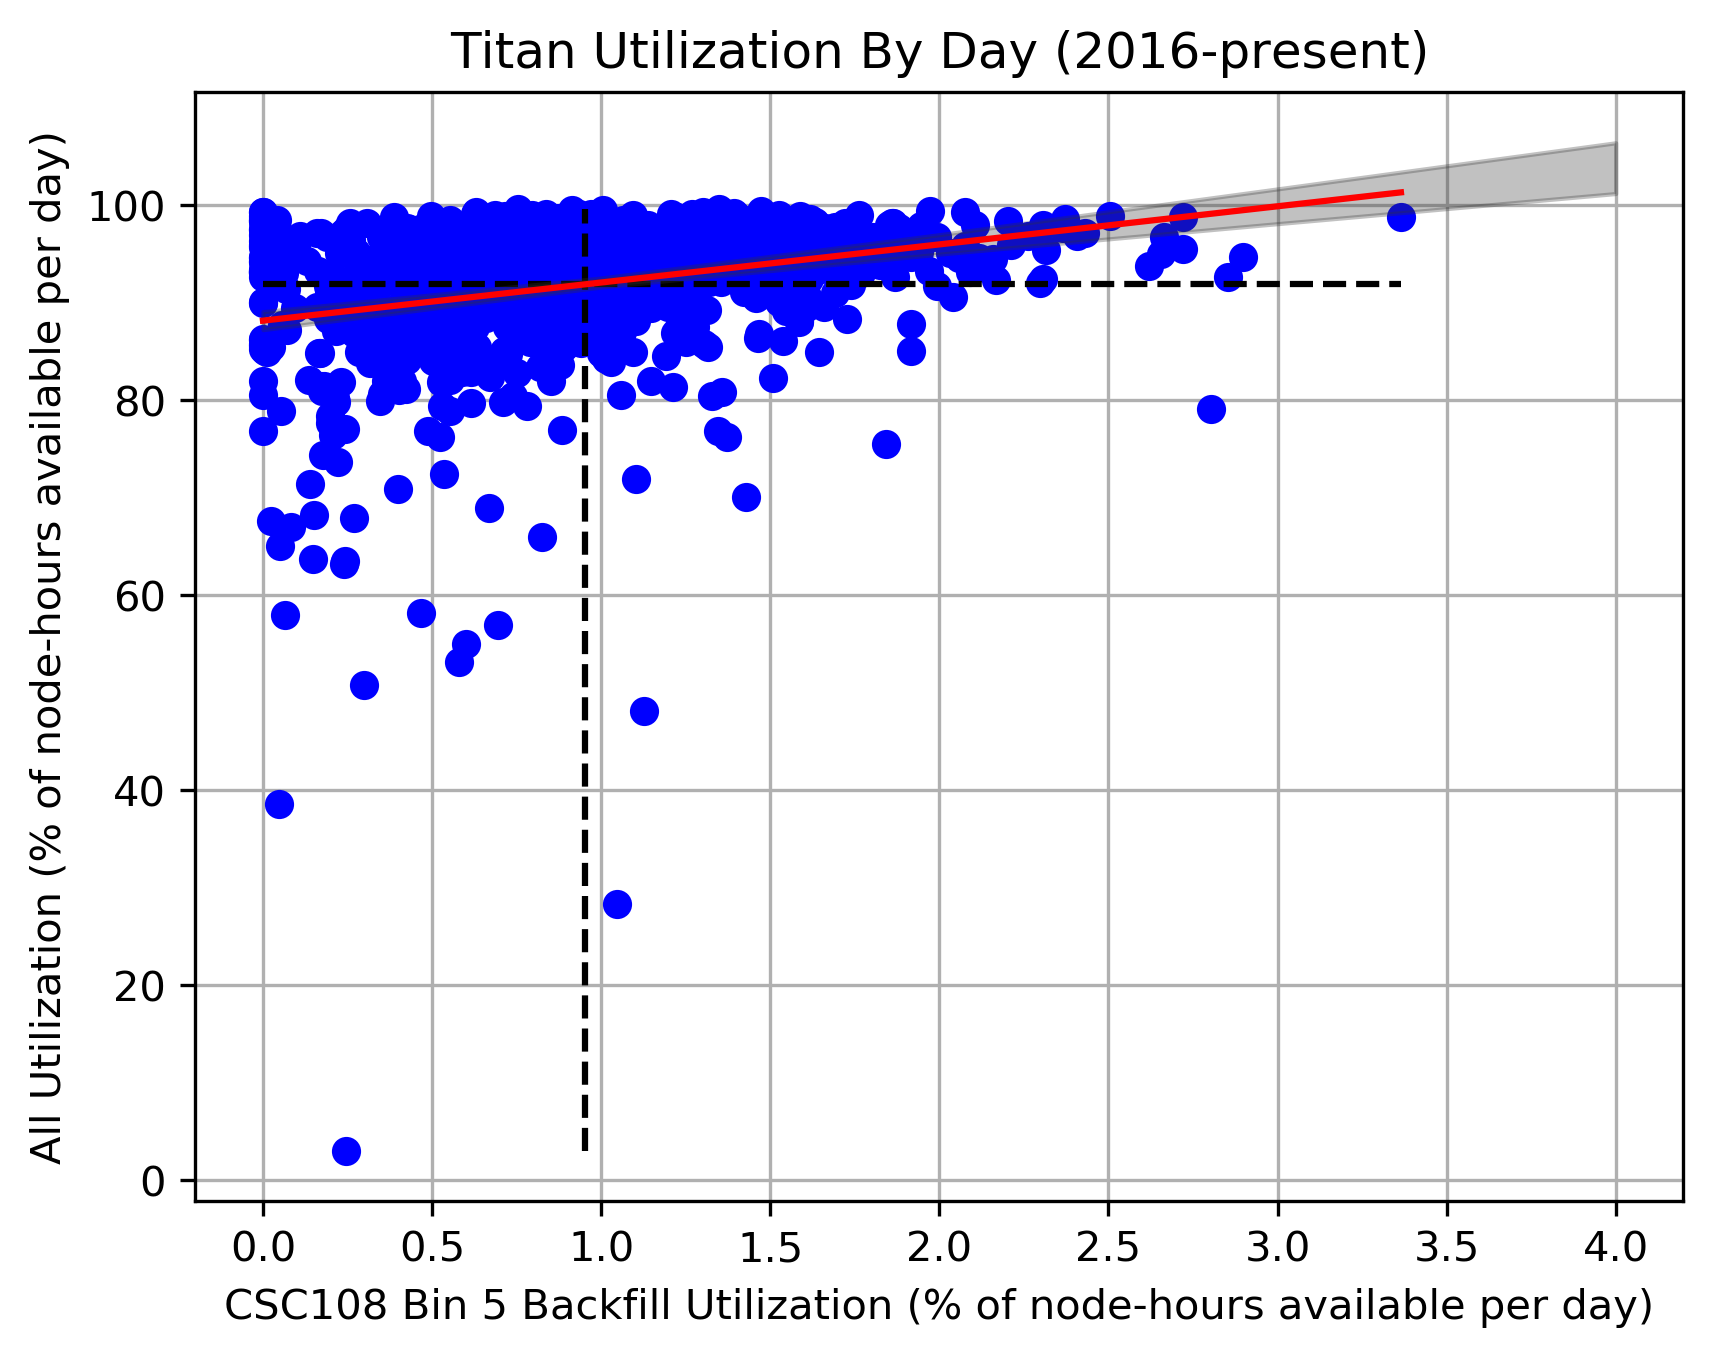
\includegraphics[width=0.4\textwidth]{images/linfit-utilization-by-true-day-bin5.png}}
  \caption{This figure demonstrates the relationship between CSC108 backfill
utilization and overall utilization on Titan, as percentages of available
node-hours each day. Each blue point represents one day. Each red line is an
Ordinary Least Squares (OLS) linear regression with parameters given in
Table~\ref{tab:utilization-params}. Each shaded gray area represents a 95\%
confidence regions. Each horizontal dotted black line represents the mean
utilization every day on Titan, and each vertical dotted black line represents
the mean utilization of backfill opportunity every day by CSC108.}
\end{figure*}

% For tables use
\begin{table}
% table caption is above the table
\caption{The table contains the parameter values for the Ordinary Least Squares
(OLS) linear regression models regarding utilization. The first column
corresponds to the figure depicting the model, and the second column
corresponds to the OLCF bin number, as defined in Table~\ref{tab:olcf-bins}.
The second and third columns correspond the coefficients $\beta_1$ and
$\beta_0$ in the model $y = \beta_{1}x + \beta_0$.}
\label{tab:utilization-params}       % Give a unique label
% For LaTeX tables use
\begin{tabular}{ccrrr}
\hline\noalign{\smallskip}
Figure  & OLCF Bin & Slope $\beta_1$  & Intercept $\beta_0$  &  $\text{R}^2$ \\
\noalign{\smallskip}\hline\noalign{\smallskip}
\ref{fig:utilization-all}    &   All &  -0.5258 &   93.3404     &   0.0330  \\
\ref{fig:utilization-bin3}   &   3   &  -1.0977 &   94.0609     &   0.1359  \\
\ref{fig:utilization-bin4}   &   4   &  -1.1472 &   92.7870     &   0.0378  \\
\ref{fig:utilization-bin5}   &   5   &   4.3328 &   87.5839     &   0.1046  \\
\noalign{\smallskip}\hline
\end{tabular}
\end{table}
%%%

The plots shown in Figures~\ref{fig:throughput-all}, \ref{fig:throughput-bin3},
\ref{fig:throughput-bin4}, and \ref{fig:throughput-bin5} visually suggest that
CSC108 has little to no effect on other projects' throughputs, but the numbers
in Table~\ref{tab:throughput-params} show that linear relationships explain
very little of the variability in the data. The $\text{R}^2$ values, which
represent goodness-of-fit on a scale of 0 to 1, are very close to 0, indicating
poor fit.

Similar problems exist for the utilization results, but they raise one very
interesting question. The plots shown in Figures~\ref{fig:utilization-all},
\ref{fig:utilization-bin3}, and \ref{fig:utilization-bin4} are all suggestive
of an inverse relationship, but \ref{fig:utilization-bin5} suggests a direct
relationship, by virtue of its positive slope. The $R^2$ values show that
linear relationships explain very little of the variability in the data,
however, as shown in Table~\ref{tab:utilization-params}, because the
$\text{R}^2$ values are very close to 0, on a scale of 0 to 1. Thus, there are
no simple linear relationships at work here, because the goodness-of-fit values
are consistently close to 0.
\jhanote{Previous paragraph is casual and not precise. Needs fixing.}
\seannote{Agreed. I took out judgmental language and moved the opinions to be
stored in the Summary section for now.}

%%%%%%%%%%%%%%%%%%%%%%%%%%%%%%%%%%%%%%%%%%%%%%%%%%%%%%%%%%%%%%%%%%%%%%%%%%%%%%%%
\subsection{Blocking probability}
\label{subsec:blocking-probability}

The previous subsection analyzed traces for correlations between global set of
all jobs on Titan and CSC108 jobs. Although a useful exercise, the results are
at best inconclusive due to intrinsic noisiness which makes discerning
correlations even harder. In this section, we  try to model the underlying
process with the objective of moving beyond correlations and inferring casual
relationships between CSC108 scheduling events and a measure of impact
(utilization, wait time or throughput).

We begin by defining a ``block'' which is an event that occurs when an job
submitted to the batch queue is stalled in the wait state even though there
might be sufficient resources to run that job. A block typically occurs due to
some other job(s) using resources, and therefore the otherwise eligible job
has been ``blocked'' by an already-running job. A blocking event is
interesting because it indicates interference between jobs and competition for
resources even in the presence of available resources. A systematic analysis
of CSC108 has the potential to determine its impact on non-CSC108 jobs.

The data used for this experiment include the same historical trace data used
in Section~\ref{subsec:rescheduling-study} and the daily availability
data for Titan used in Section~\ref{subsec:simple-linear-relationships}, but
this time are supplemented with live snapshot data of the system queue for
Titan. Snapshots were gathered by sampling live data from the Moab scheduler by
polling with Python scripts launched by cron jobs on a data transfer node.
These scripts recorded XML output from the ``showbf'' and ``showq'' commands
into files, and more cron jobs launched other Python scripts to import these
files' sample data into SQLite. These tables contain data about the exact state
of the queues at given times, including active jobs, blocked jobs, eligible
jobs, recently completed jobs, and system information such as active nodes and
available backfill opportunities. Then, experimental programs were written in
Python using the same libraries and database as the previous sections.

Formally, the definitions for a block and a blocking probability follow. Let
$C_i$ be the abstract resources in use by CSC108 at the $i^{\text{th}}$ sample
point in time, and let $U_i$ be the unused (idle) resources remaining on
Titan. We then define a boolean $B_i$ representing a ``block'' event to occur
if there exists at least one job at the $i^{\text{th}}$ sample point which
requests $(C_i + U_i)$ resources or less (when $C_i$ is non-zero). If there is
no job at $i^{\text{th}}$ which requests more than $(C_i + U_i)$ we say a
blocking event $B_i$  does not occur. Summing $B_i$ over all $i$ gives a count
of the number of blocking events that occur, and dividing that count by the
number of total sample points yields a quantity we call a ``blocking
probability''.

Informally, blocking probability represents the proportion of samples 
\jhanote{sample of what? time? intervals possibly better term?} in which a
block occurred. The idea here is that when blocking probability increases, it
indicates that the system is experiencing greater competition for its
resources. Blocking probability does not predict the probability that a
particular job will be blocked, but rather the probability that a given sample
will contain a block.

To apply this abstract model to a real data set, we have initially defined the
resources in one-dimensional ``spatial'' and ``temporal'' manners, by
considering only jobs' requested numbers of nodes in the former and only jobs'
requested wall times in the latter. An eligible job in the batch queue is said
to be spatially blocked when the job’s number of requested nodes is too large
to fit within the nodes available through backfill opportunity, so that the job
must wait to run. Similarly, an eligible job in the batch queue is said to be
temporally blocked when the job’s requested wall time is too long to fit within
the duration available through backfill opportunity. Similarly, a job is said
to be blocked ``due to CSC108'' if at least one job which was blocked would no
longer be blocked if CSC108's jobs were removed. Thus, a job is only said to be
blocked due to CSC108 if it requests resources with are greater than $U_i$ but
less than $(C_i + U_i)$. Figures
\ref{fig:spatial-blocking-by-month} and \ref{fig:temporal-blocking-by-month}
demonstrate how spatial and temporal blocking probabilities vary from month to
month, and Figure~\ref{fig:spatial-vs-temporal} shows that the two quantities
relate to each other in an intuitive way, namely, that time periods of greater
spatial blocking often correspond to time periods of greater temporal blocking
as well.

%%%
% WAIT TIMES AS SUBFIGURES
\begin{figure*}
  \subfloat[Spatial blocking\label{fig:spatial-blocking-by-month}]{
    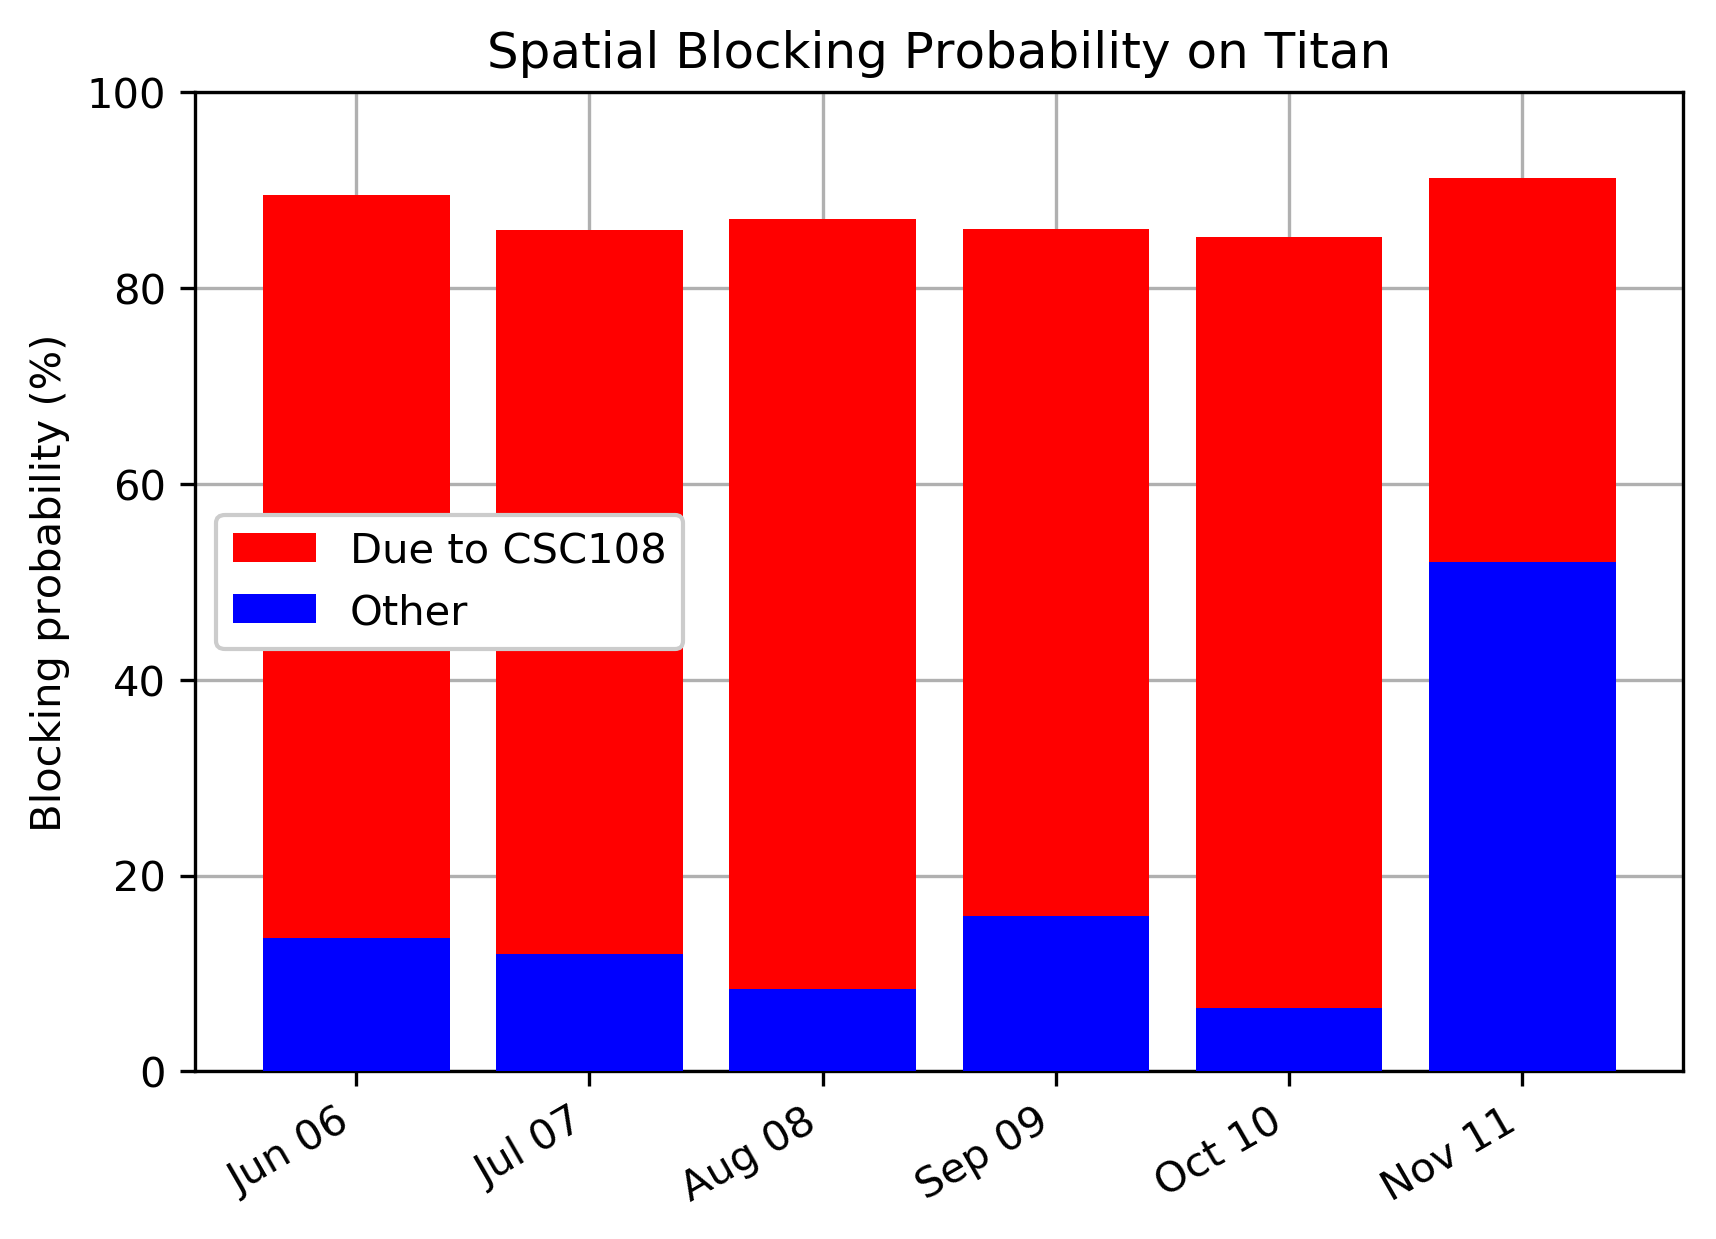
\includegraphics[width=0.4\textwidth]{images/barplot-spatial-blocking-by-month.png}}
  \subfloat[Temporal blocking\label{fig:temporal-blocking-by-month}]{
    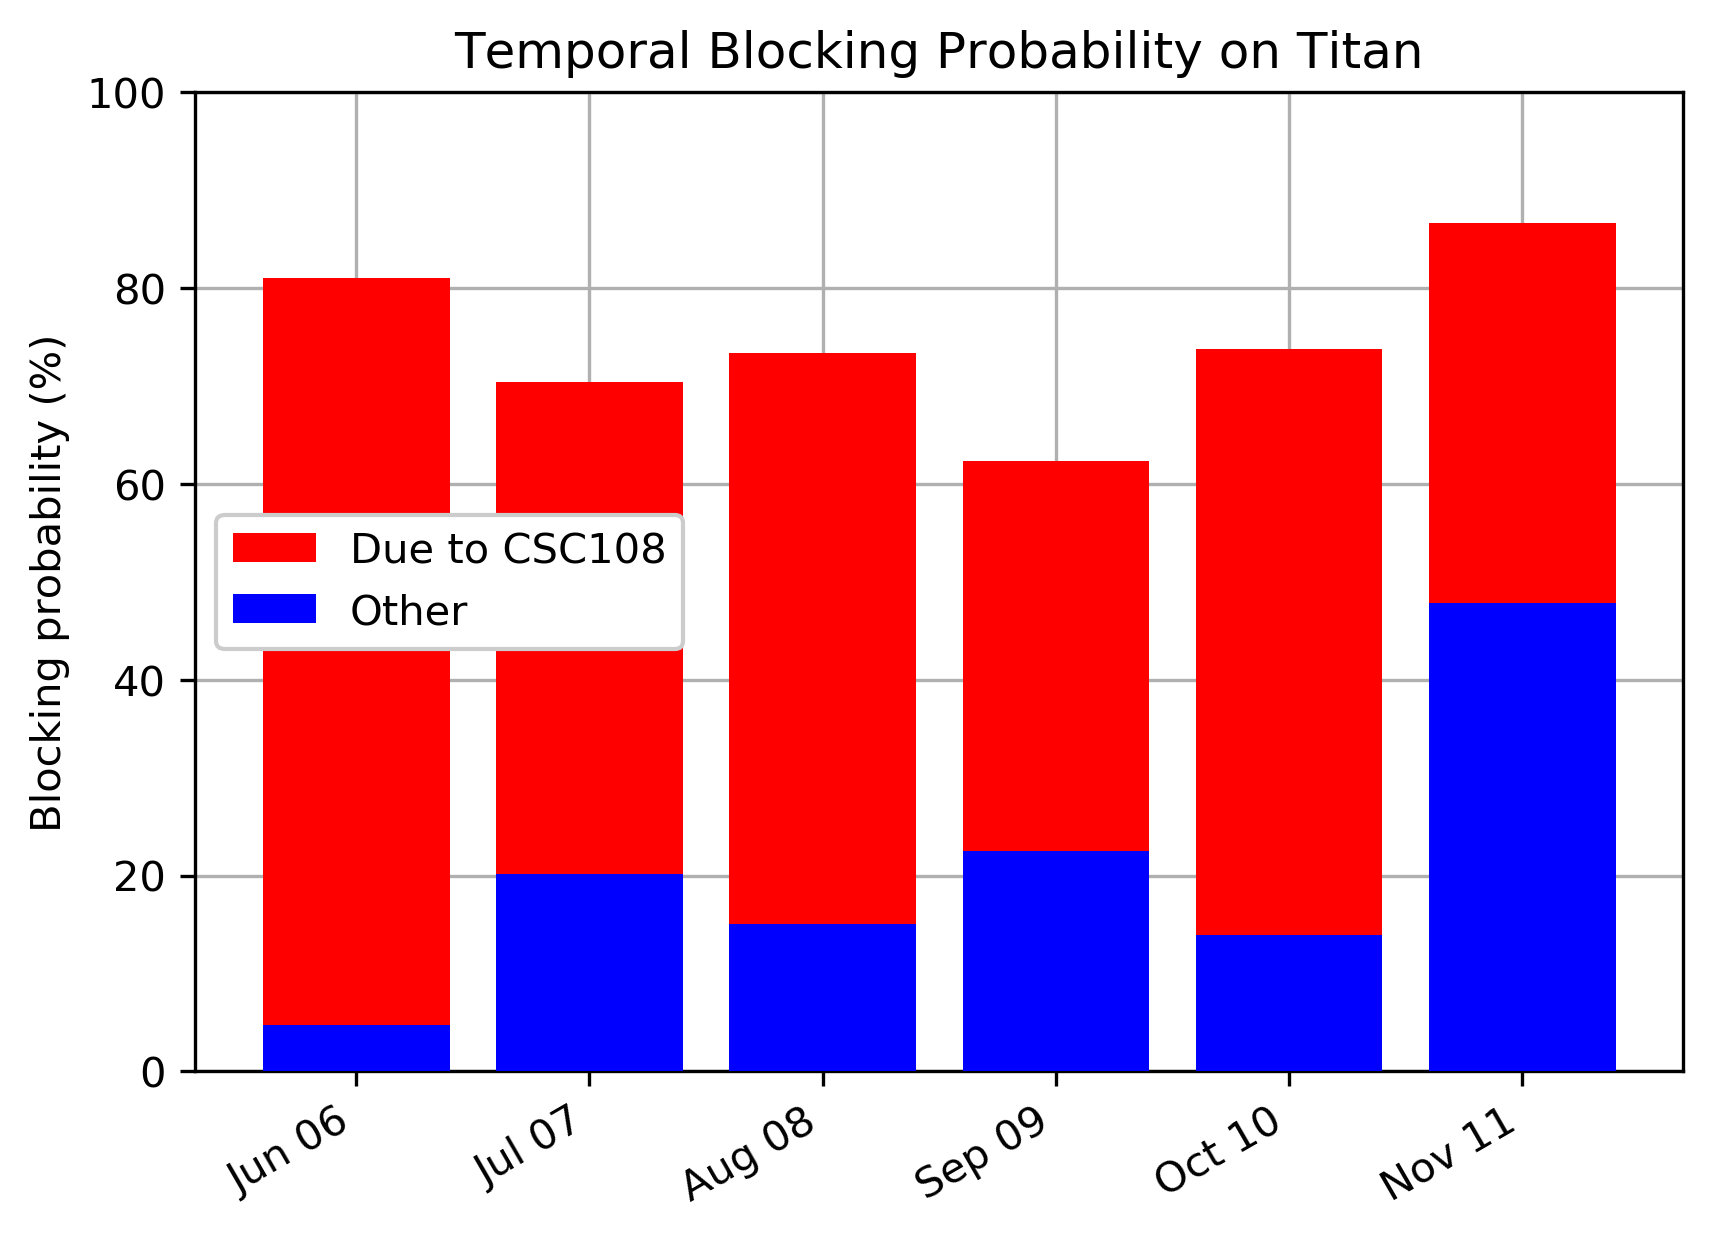
\includegraphics[width=0.4\textwidth]{images/barplot-temporal-blocking-by-month.png}}
  \caption{These plots depict the spatial and temporal blocking probabilities
by month for samples in which CSC108 was actively utilizing backfill
opportunity. The total height of the bars indicates the blocking probability
for the month, which is the proportion of samples in which at least one
eligible job was blocked. The red region indicates the percentage of samples in
which at least one eligible job would no longer be blocked if CSC108's jobs
were removed.}
\end{figure*}

% For two-column wide figures use
\begin{figure*}
% Use the relevant command to insert your figure file.
% For example, with the graphicx package use
  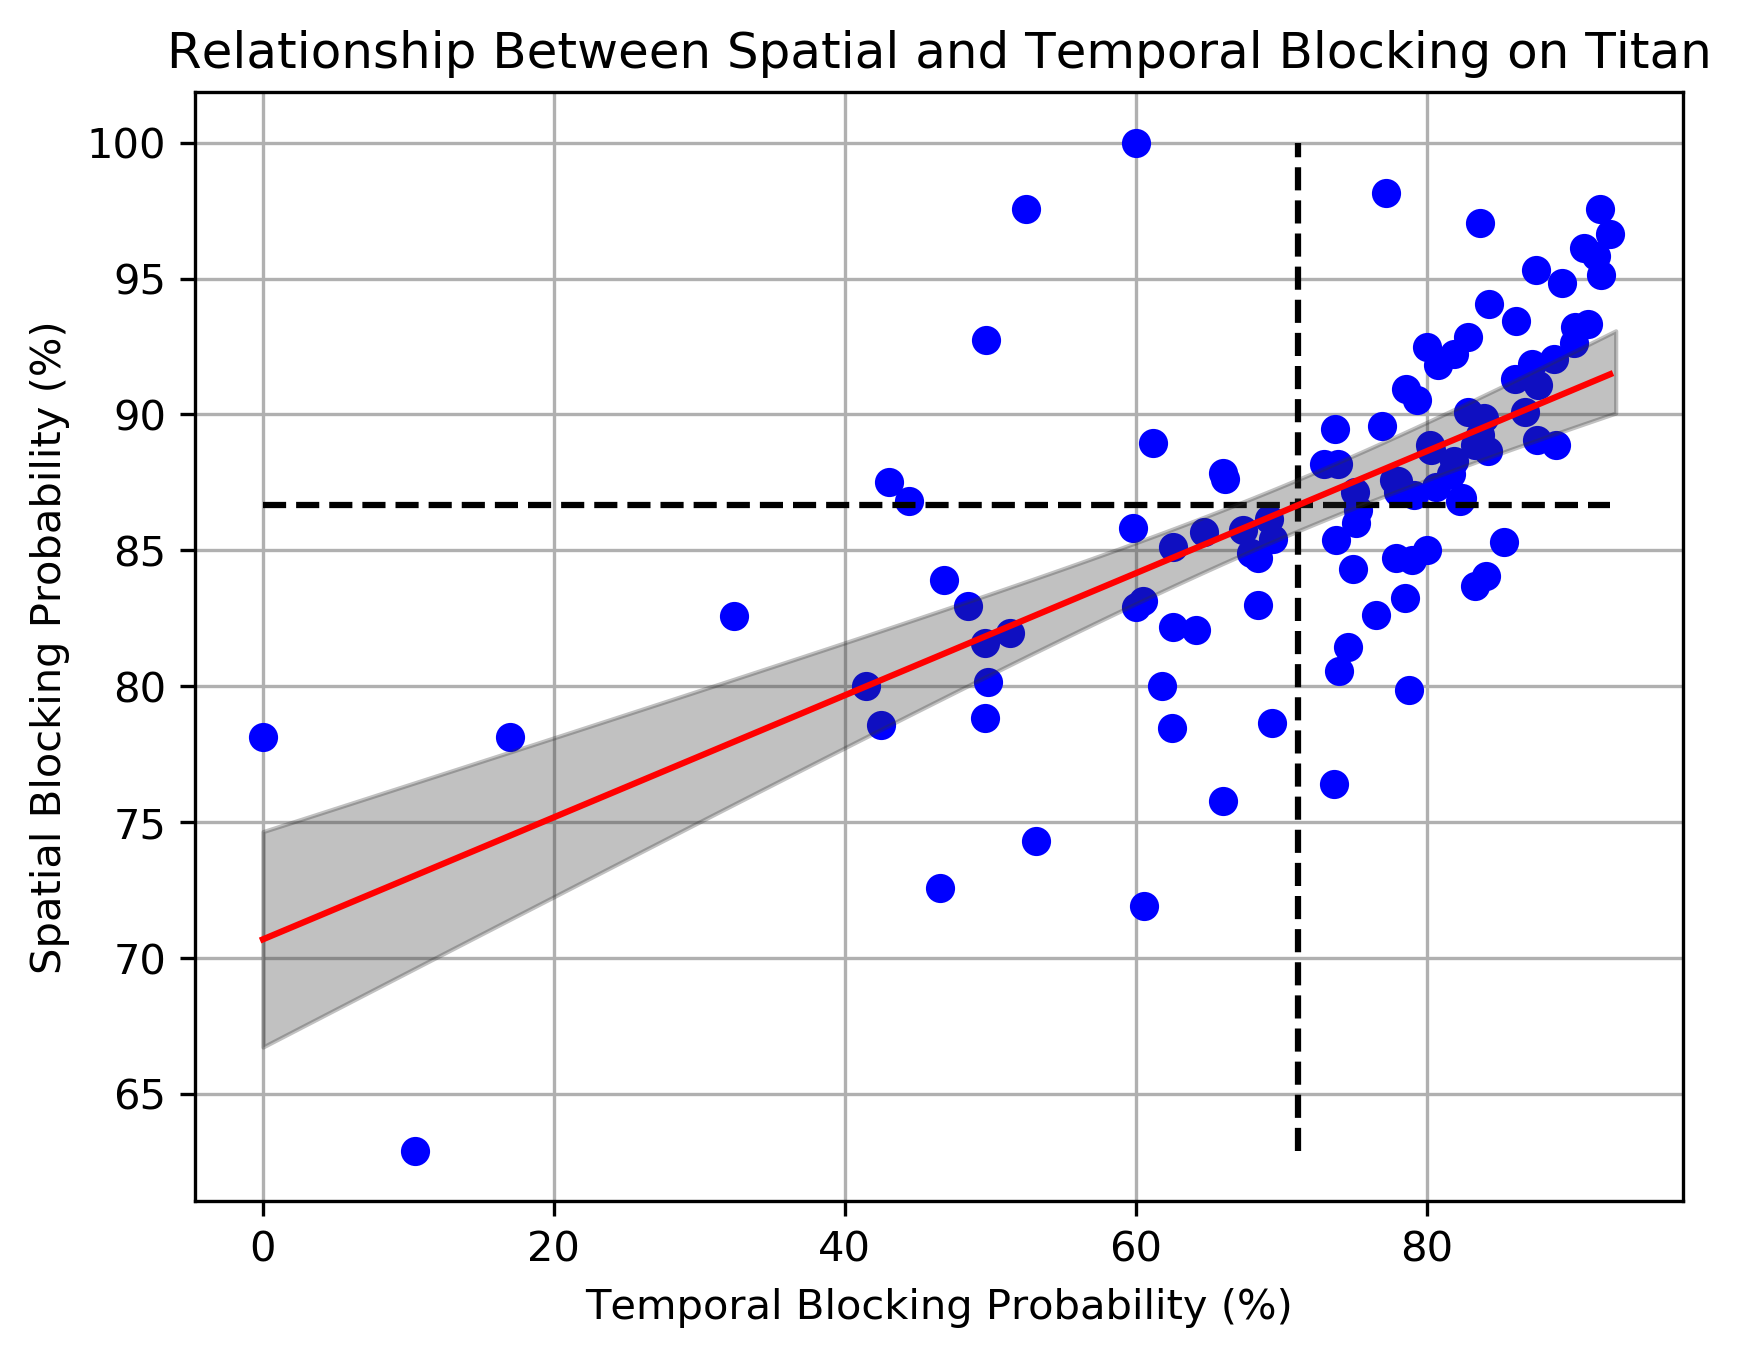
\includegraphics[width=0.75\textwidth]{images/linfit-spatial-vs-temporal-by-day.png}
% figure caption is below the figure
\caption{This figure demonstrates the relationship between spatial and temporal
blocking probabilities. Each blue point represents one day. The red line is an
Ordinary Least Squares (OLS) linear regression ($y = \beta_{1}x + \beta_0$)
with a slope $\beta_1$ of 0.2503 and an intercept $\beta_0$ of 68.7731. The
shaded gray areas represent 95\% confidence regions. The horizontal dotted
black line represents the mean spatial blocking probability for all points, and
the vertical dotted black line represents the mean temporal blocking
probability for all points. The $\text{R}^2$ value is 0.4410.}
\label{fig:spatial-vs-temporal}
\end{figure*}
%%%

Three indicators of system performance were chosen this time, as well, to
assess the impact of CSC108 on Titan: wait times, throughput, and utilization.
In order to map wait time to a value that can be attributed to a day, wait time
was defined in terms of an average wait time. Average wait time was defined as
the total number of hours spent waiting during a given day, per job that
appeared on that day. For example, a job which was submitted one day but which
did not run until the next day would contribute part of its wait time to the
first day and the rest to the second day, and it would be considered to have
appeared on both days. Throughput was defined as the number of jobs completed
per day, as before. Utilization was also defined as before, as the percentage
of core hours consumed out of the total core hours available.

%%% WAIT TIMES STUFF

Having established the two measures of blocking probability and their
relationship to one another, we followed the same techniques used in
Section~\ref{subsec:simple-linear-relationships} to create best-fit lines with
95\% confidence intervals, to investigate the relationships between blocking
probabilities and wait times experienced by jobs on Titan. Figures
\ref{fig:wait-time-spatial-all} and \ref{fig:wait-time-temporal-all} illustrate
the effects of spatial and temporal blocking probability on wait times, and
Figures \ref{fig:wait-time-spatial-csc108} and
\ref{fig:wait-time-temporal-csc108} show how CSC108's contribution to blocking
impacts wait times. More specifically, in Figures
\ref{fig:wait-time-spatial-csc108} and \ref{fig:wait-time-temporal-csc108}, the
values used for the blocking probabilities correspond to the red regions in
Figures \ref{fig:spatial-blocking-by-month} and
\ref{fig:temporal-blocking-by-month}, which indicate the percentage of samples
in which at least one eligible job would no longer be blocked if CSC108 freed
its resources. The qualitative interpretation for the wait time plots is that,
as competition for resources increases on Titan, average wait times decrease,
but when competition with CSC108 for nodes increases, average wait times
increase. Unfortunately, the goodness-of-fit values are again very poor.

\begin{figure*}
  \subfloat[Spatial blocking\label{fig:wait-time-spatial-all}]{
    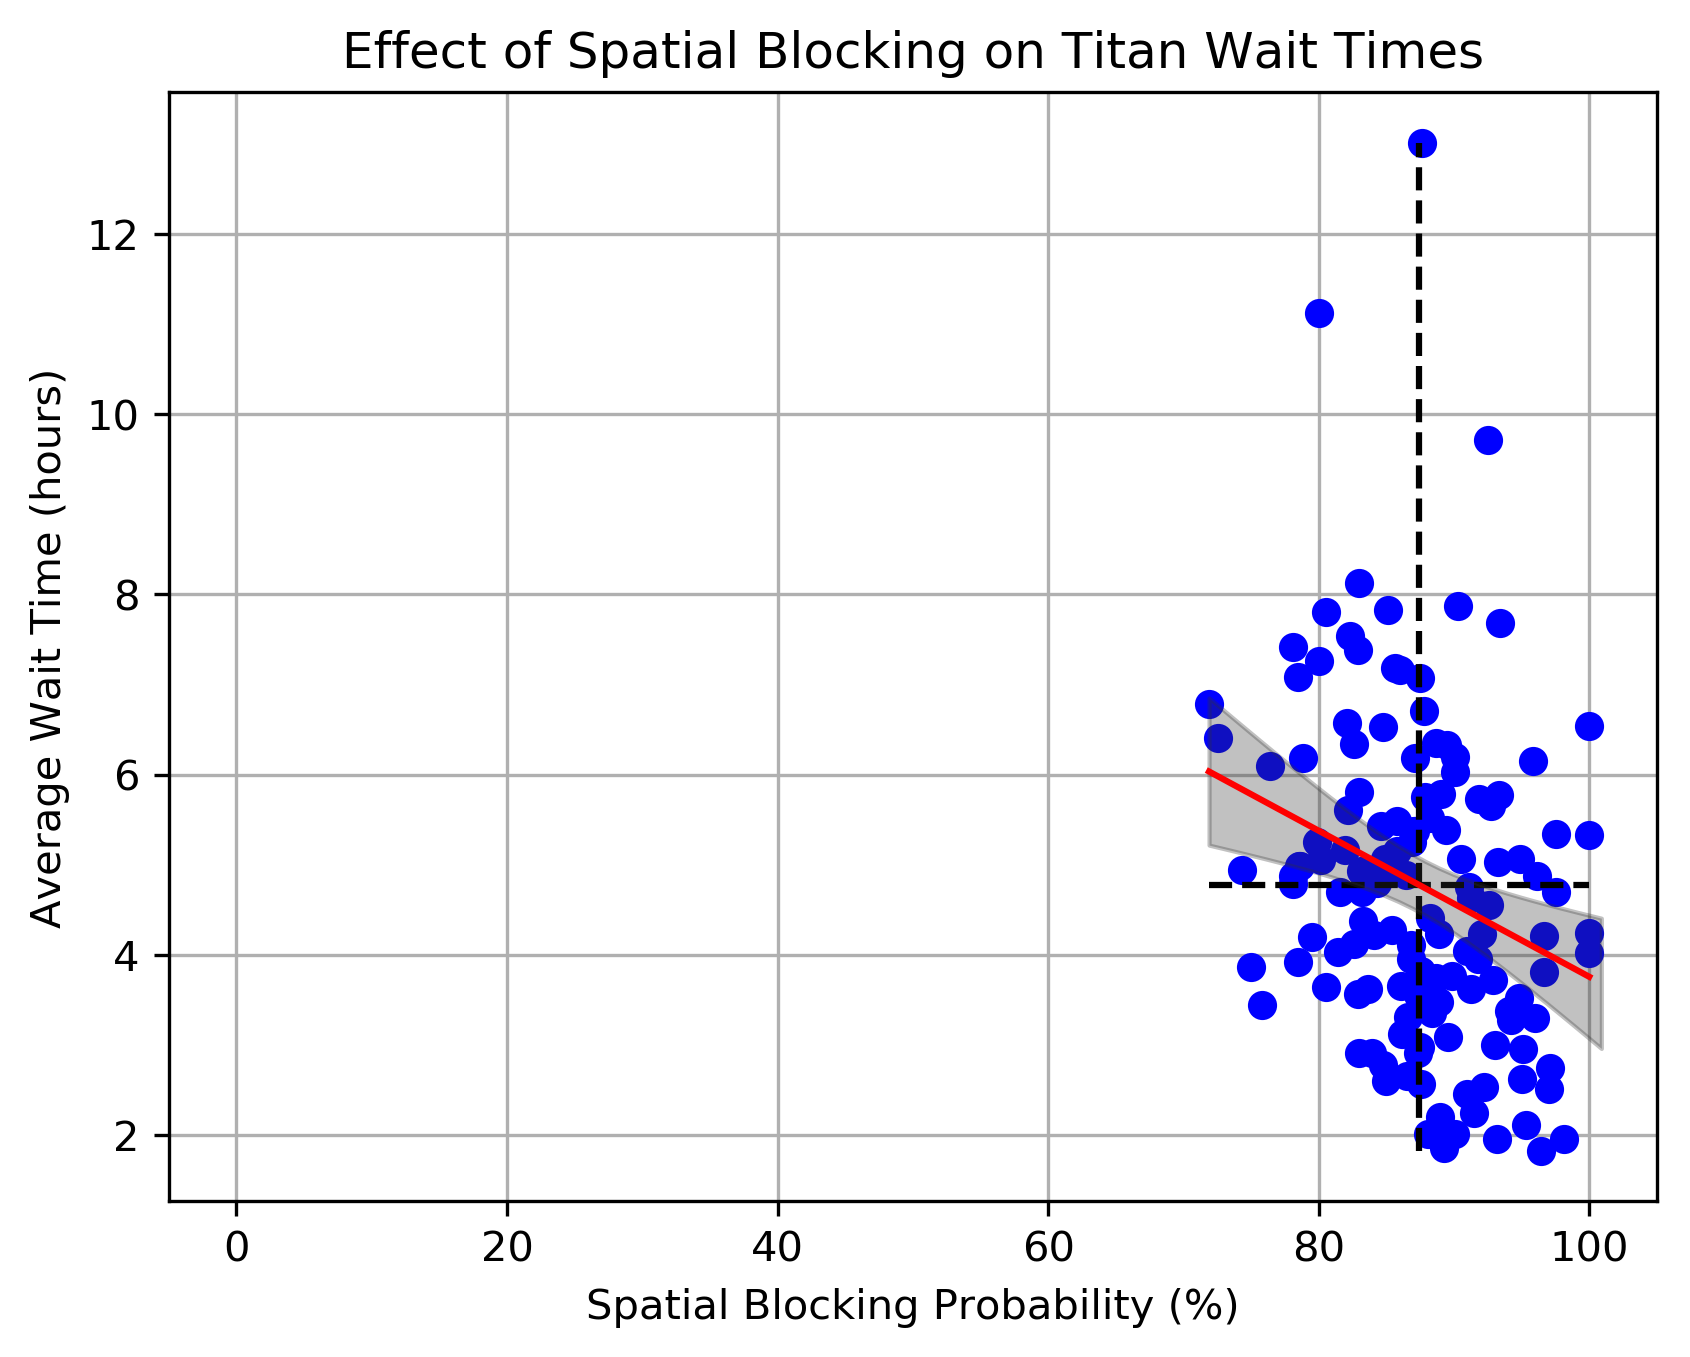
\includegraphics[width=0.4\textwidth]{images/linfit-wait-time-vs-spatial-blocking-by-day.png}}
  \subfloat[Temporal blocking\label{fig:wait-time-temporal-all}]{
    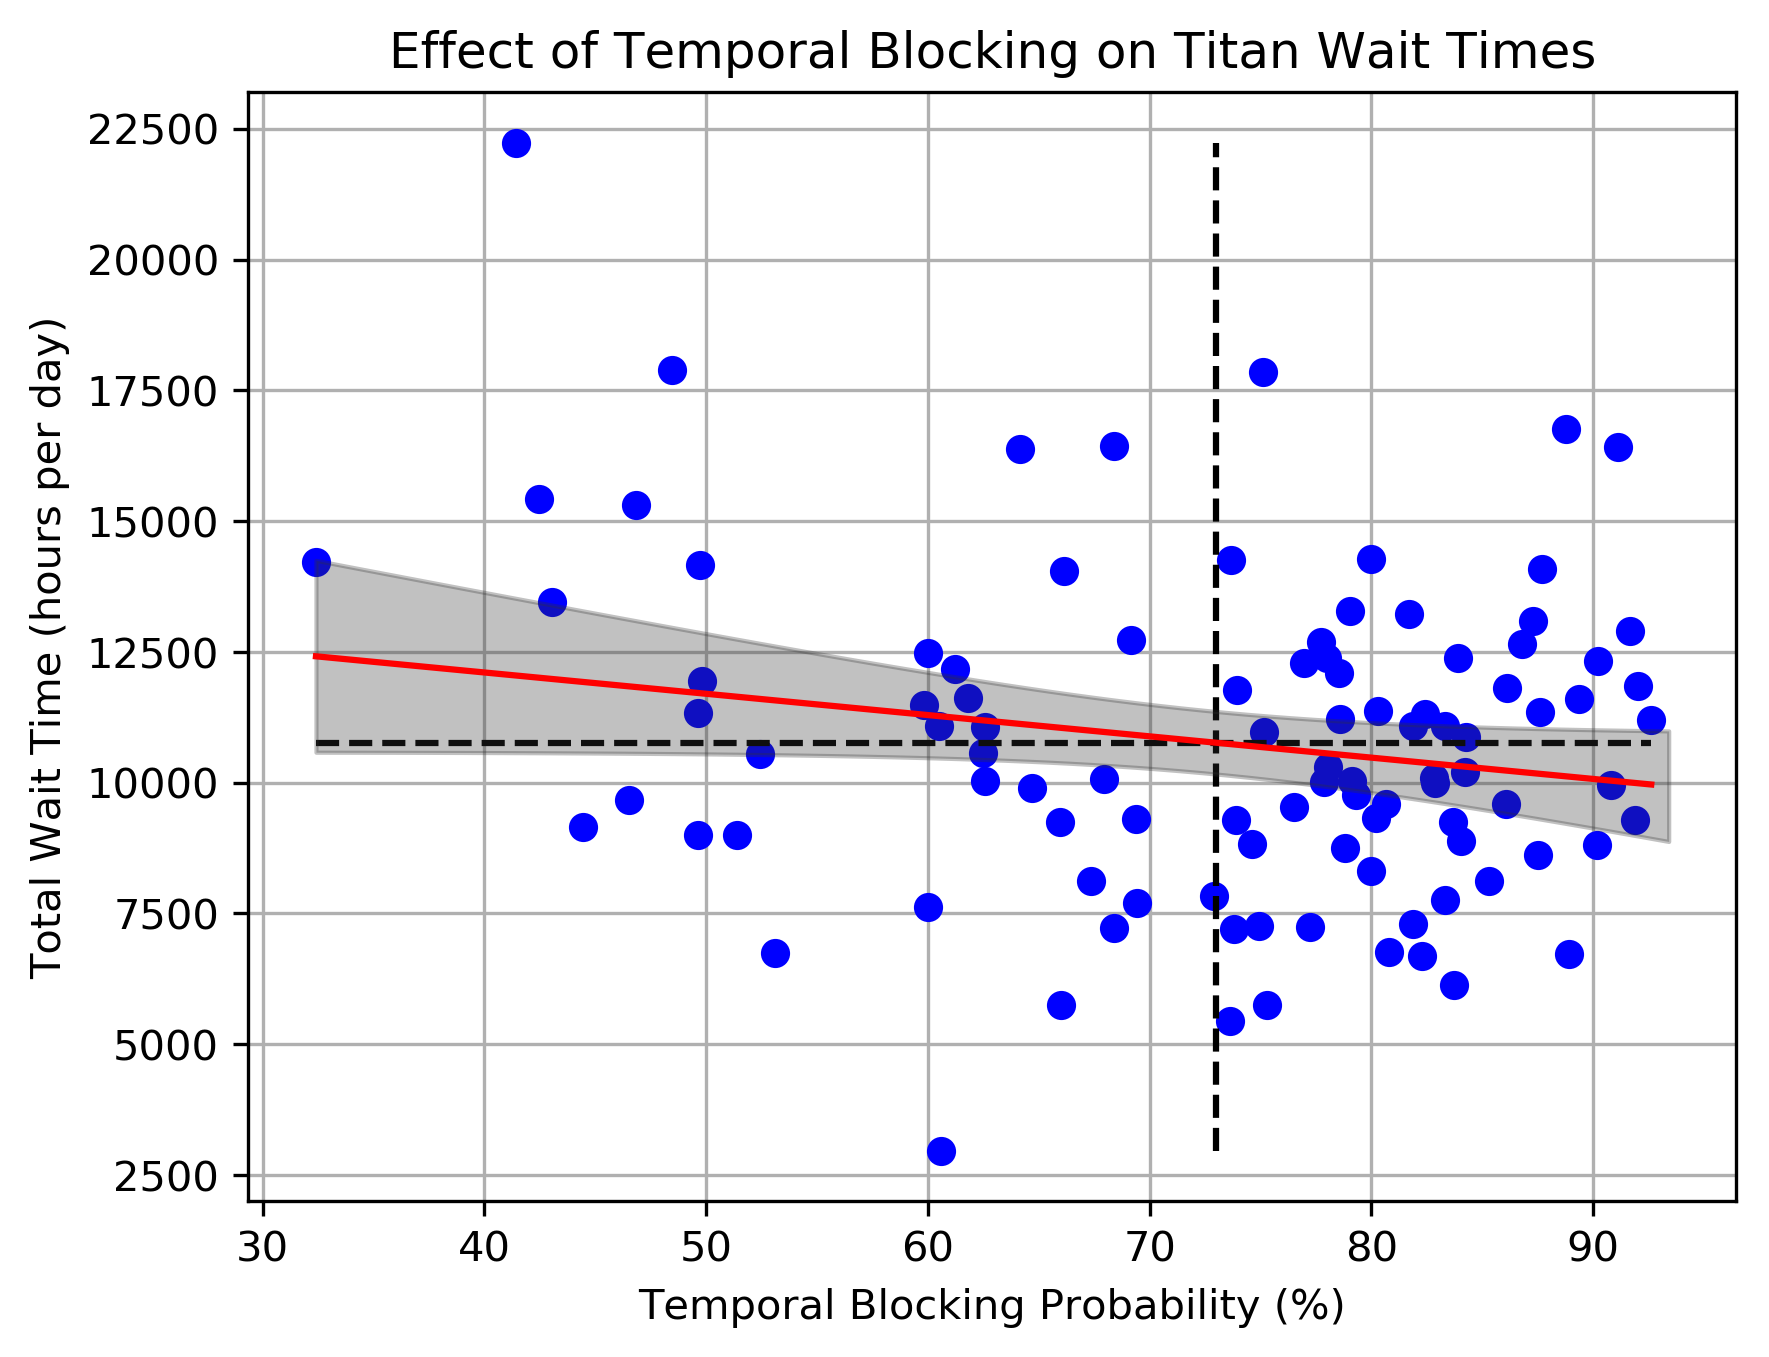
\includegraphics[width=0.4\textwidth]{images/linfit-wait-time-vs-temporal-blocking-by-day.png}}
  \vspace{1em}
  \subfloat[Spatial blocking by CSC108\label{fig:wait-time-spatial-csc108}]{
    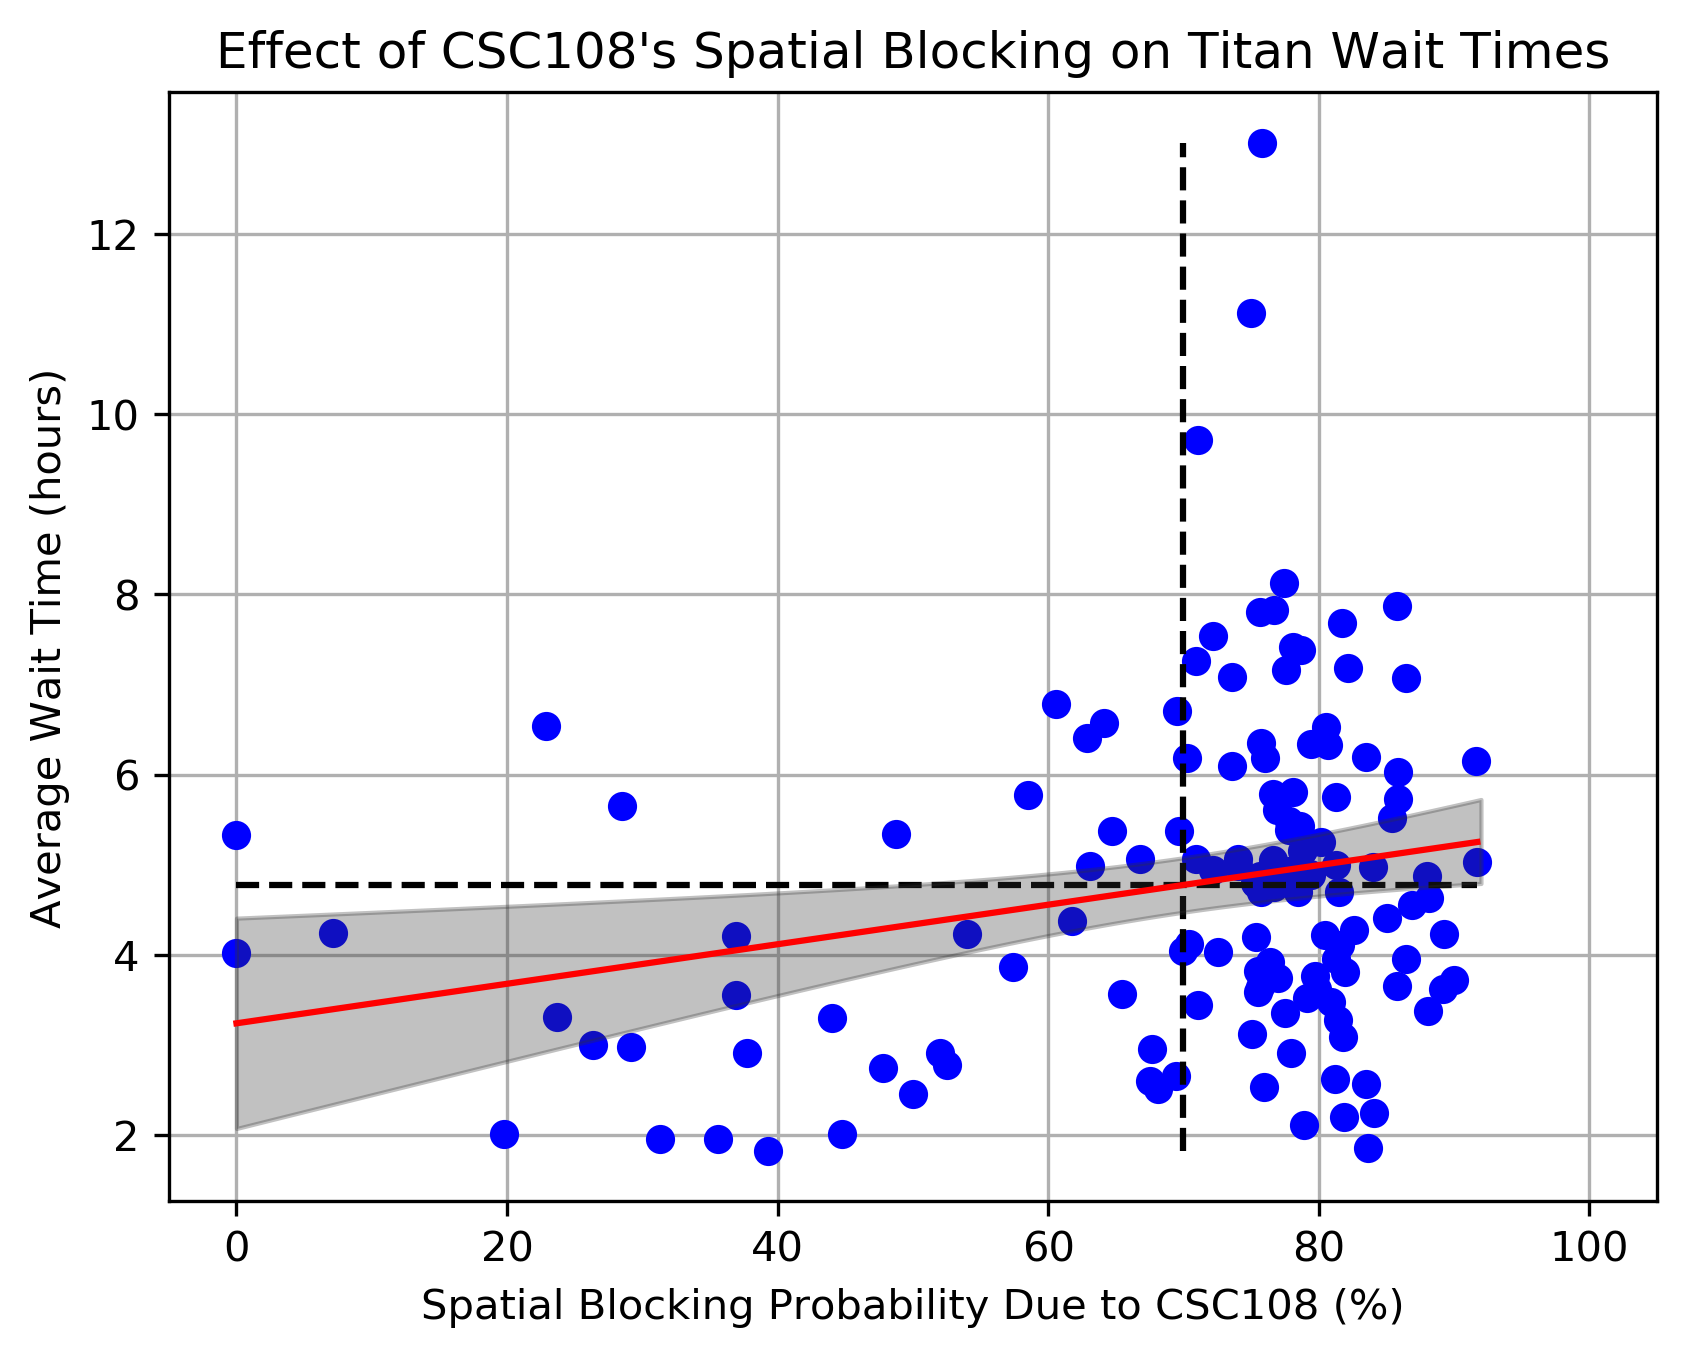
\includegraphics[width=0.4\textwidth]{images/linfit-wait-time-vs-csc108-spatial.png}}
  \subfloat[Temporal blocking by CSC108\label{fig:wait-time-temporal-csc108}]{
    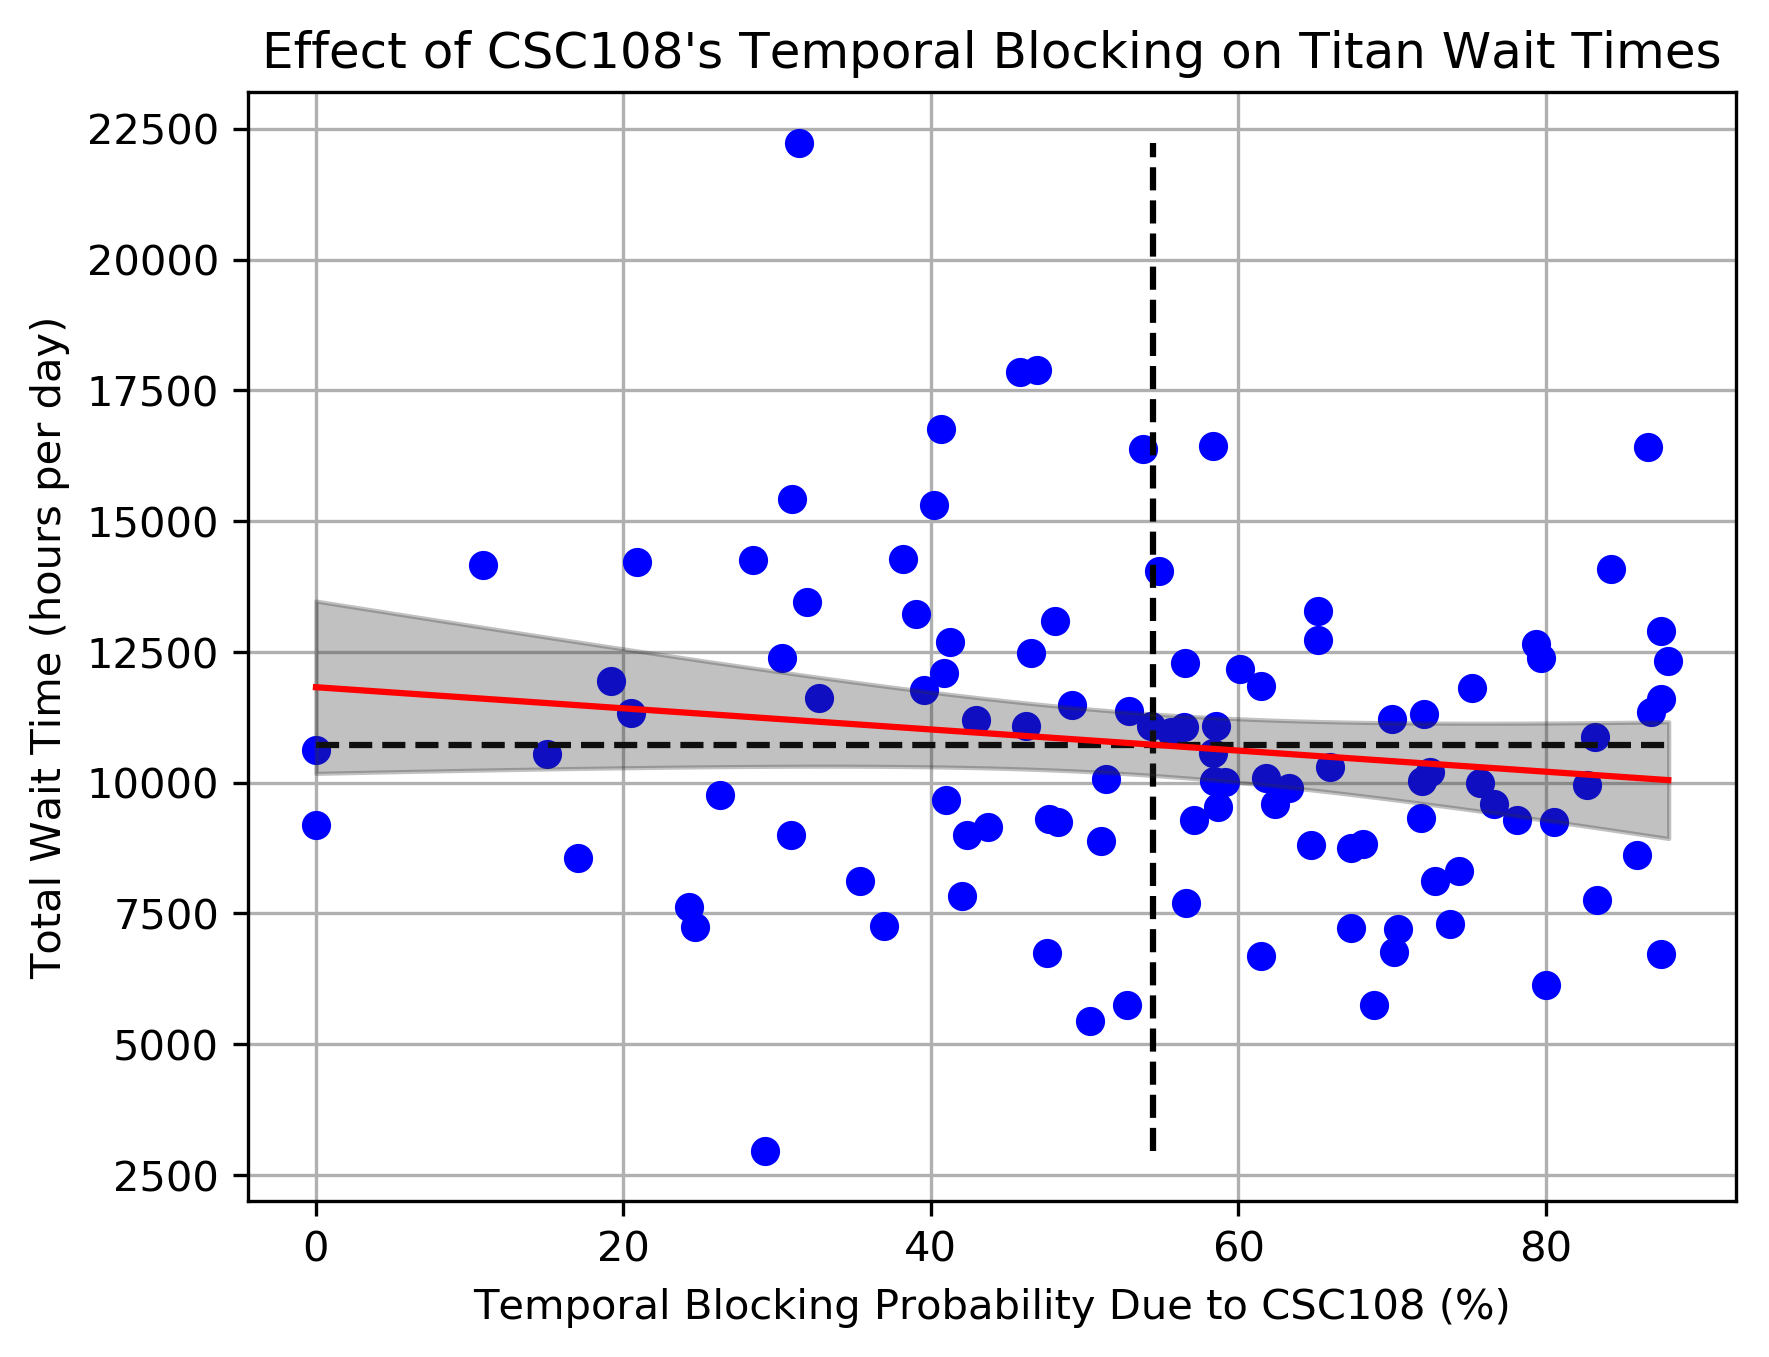
\includegraphics[width=0.4\textwidth]{images/linfit-wait-time-vs-csc108-temporal.png}}
  \caption{These plots demonstrate the relationships between the average wait
times on Titan and one-dimensional blocking probabilities. Each blue point
represents one day. Each red line is an Ordinary Least Squares (OLS) linear
regression with parameters given in Table~\ref{tab:blocking-wait-time-params}.
Each shaded gray area represents a 95\% confidence region. Each horizontal
dotted black line represents the mean wait times for all points in that plot,
and each vertical dotted black line represents the mean blocking probability
for all points in that plot.}
\end{figure*}

% For tables use
\begin{table}
% table caption is above the table
\caption{The table contains the parameter values for the Ordinary Least Squares
(OLS) linear regression models regarding blocking probabilities and average
wait times. The first column corresponds to the figure depicting the model,
while the second and third columns correspond the coefficients $\beta_1$ and
$\beta_0$ in the model $y = \beta_{1}x + \beta_0$.}
\label{tab:blocking-wait-time-params}       % Give a unique label
% For LaTeX tables use
\begin{tabular}{crrr}
\hline\noalign{\smallskip}
Figure  & Slope $\beta_1$ & Intercept $\beta_0$     & $\text{R}^2$ \\
\noalign{\smallskip}\hline\noalign{\smallskip}
\ref{fig:wait-time-spatial-all}     &   -0.0810 &   11.8610 &   0.0737  \\
\ref{fig:wait-time-temporal-all}    &   -0.0401 &    7.7491 &   0.1265  \\
\ref{fig:wait-time-spatial-csc108}  &    0.0219 &    3.2420 &   0.0509  \\
\ref{fig:wait-time-temporal-csc108} &   -0.0102 &    5.3217 &   0.0147  \\
\noalign{\smallskip}\hline
\end{tabular}
\end{table}

%%% THROUGHPUT STUFF

Figures \ref{fig:throughput-spatial-all}, \ref{fig:throughput-temporal-all},
\ref{fig:throughput-spatial-csc108}, and \ref{fig:throughput-temporal-csc108}
are all in agreement that increasing competition corresponds to increasing
throughput, in units of jobs completed per day. The goodness-of-fit values are
poor, however, as shown in Table~\ref{tab:blocking-throughput-params}, so these qualitative results may only be said to be suggestive.

%%%
\begin{figure*}
  \subfloat[Spatial blocking\label{fig:throughput-spatial-all}]{
    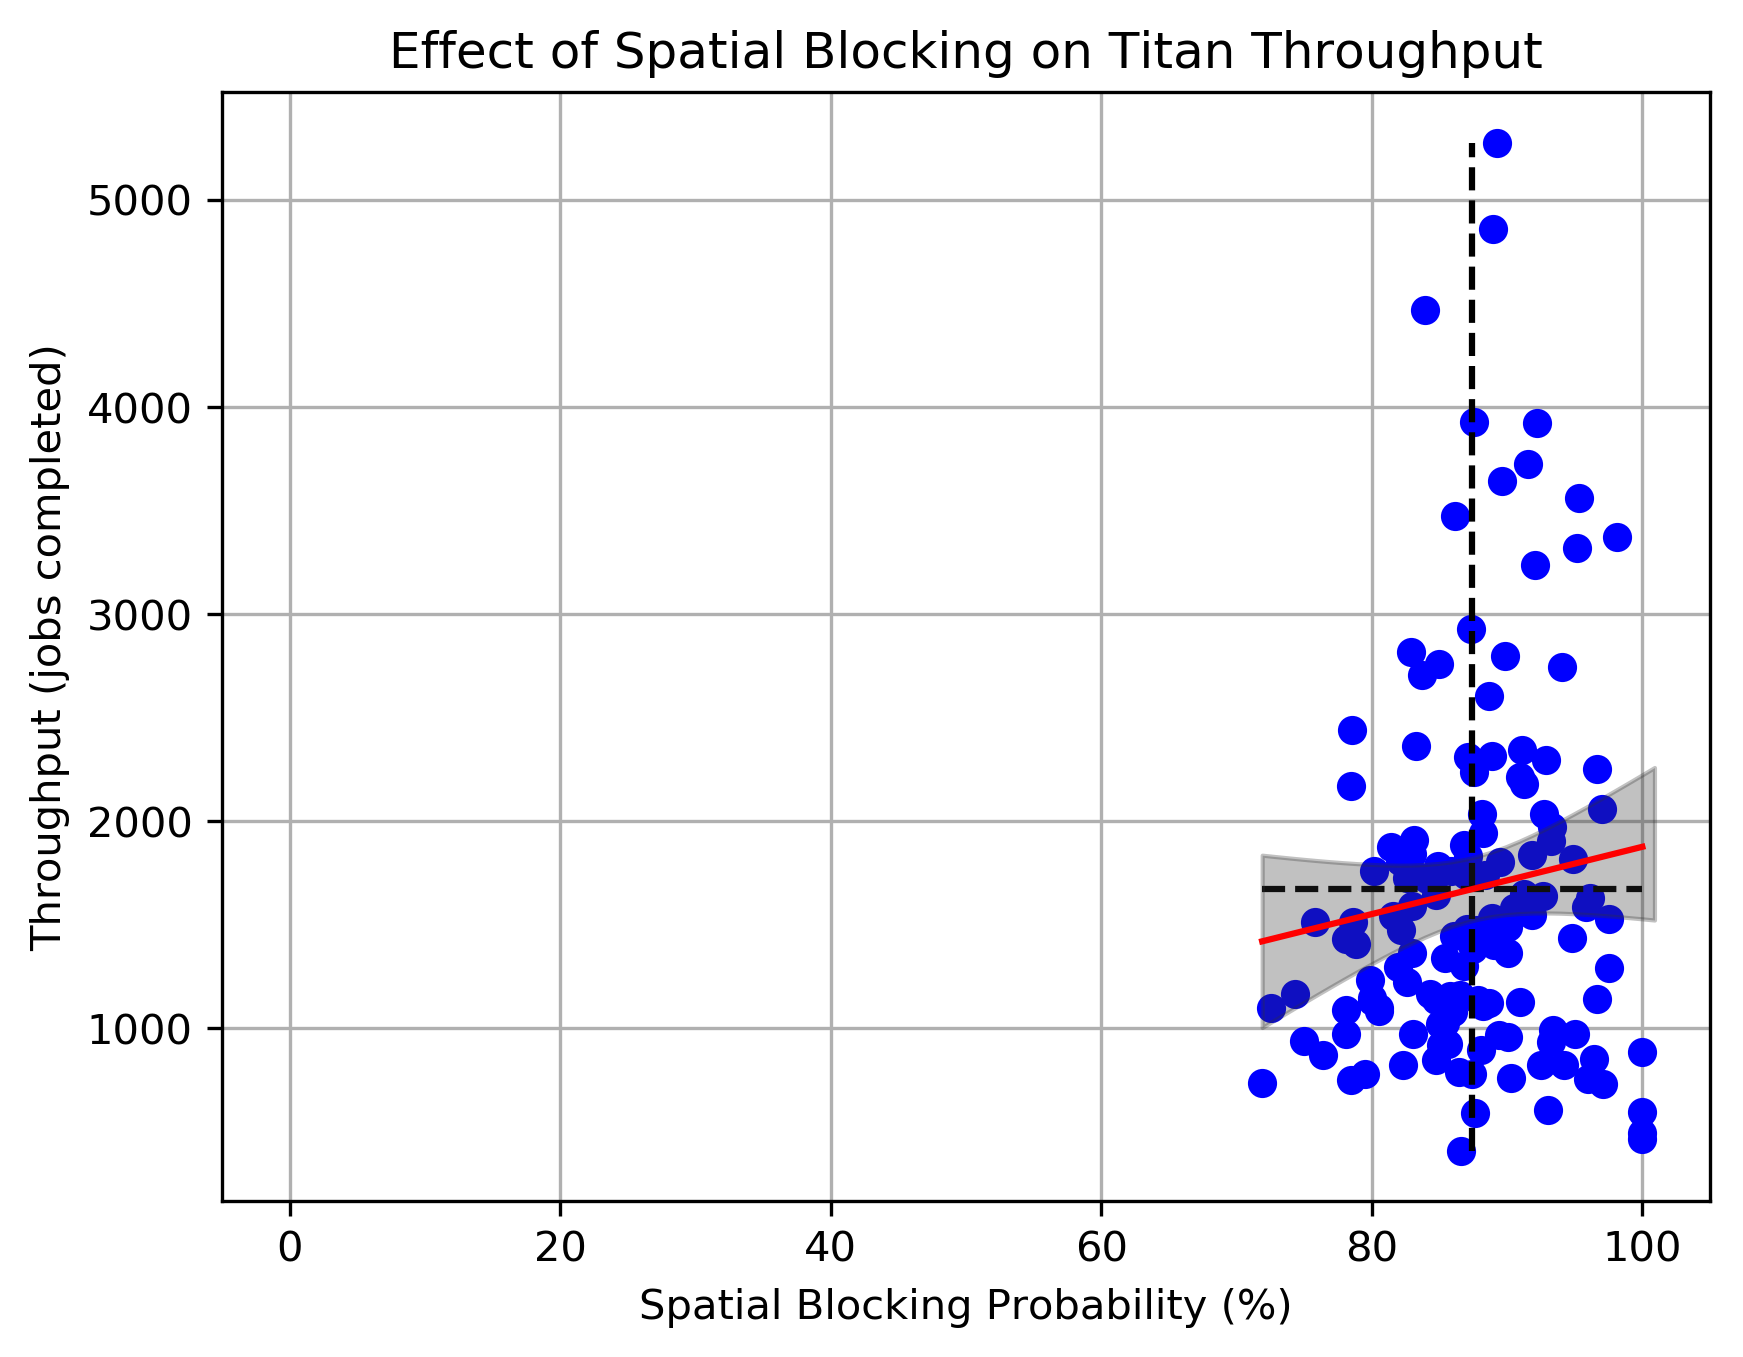
\includegraphics[width=0.4\textwidth]{images/linfit-throughput-vs-spatial-blocking.png}}
  \subfloat[Temporal blocking\label{fig:throughput-temporal-all}]{
    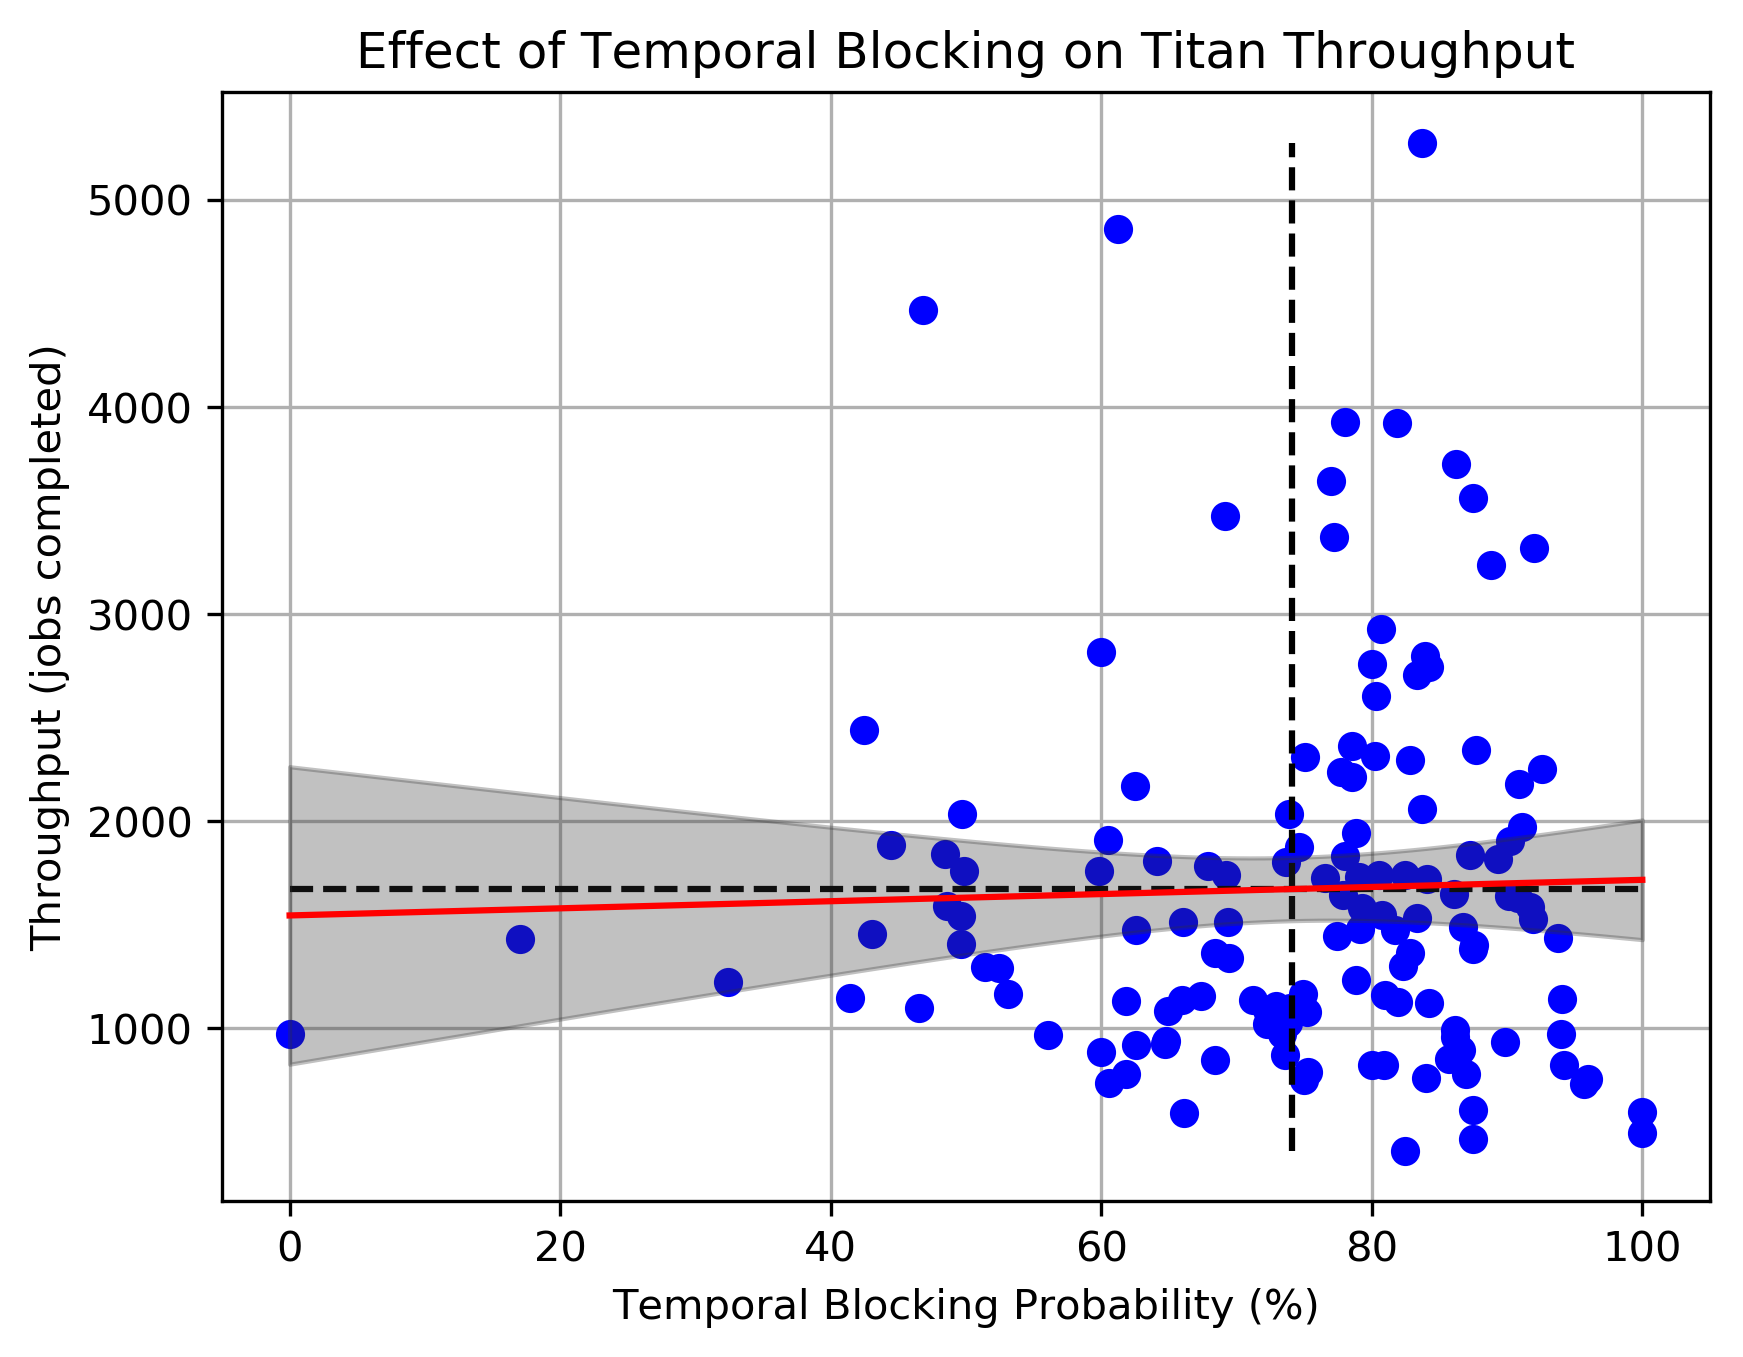
\includegraphics[width=0.4\textwidth]{images/linfit-throughput-vs-temporal-blocking.png}}
  \vspace{1em}
  \subfloat[Spatial blocking by CSC108\label{fig:throughput-spatial-csc108}]{
    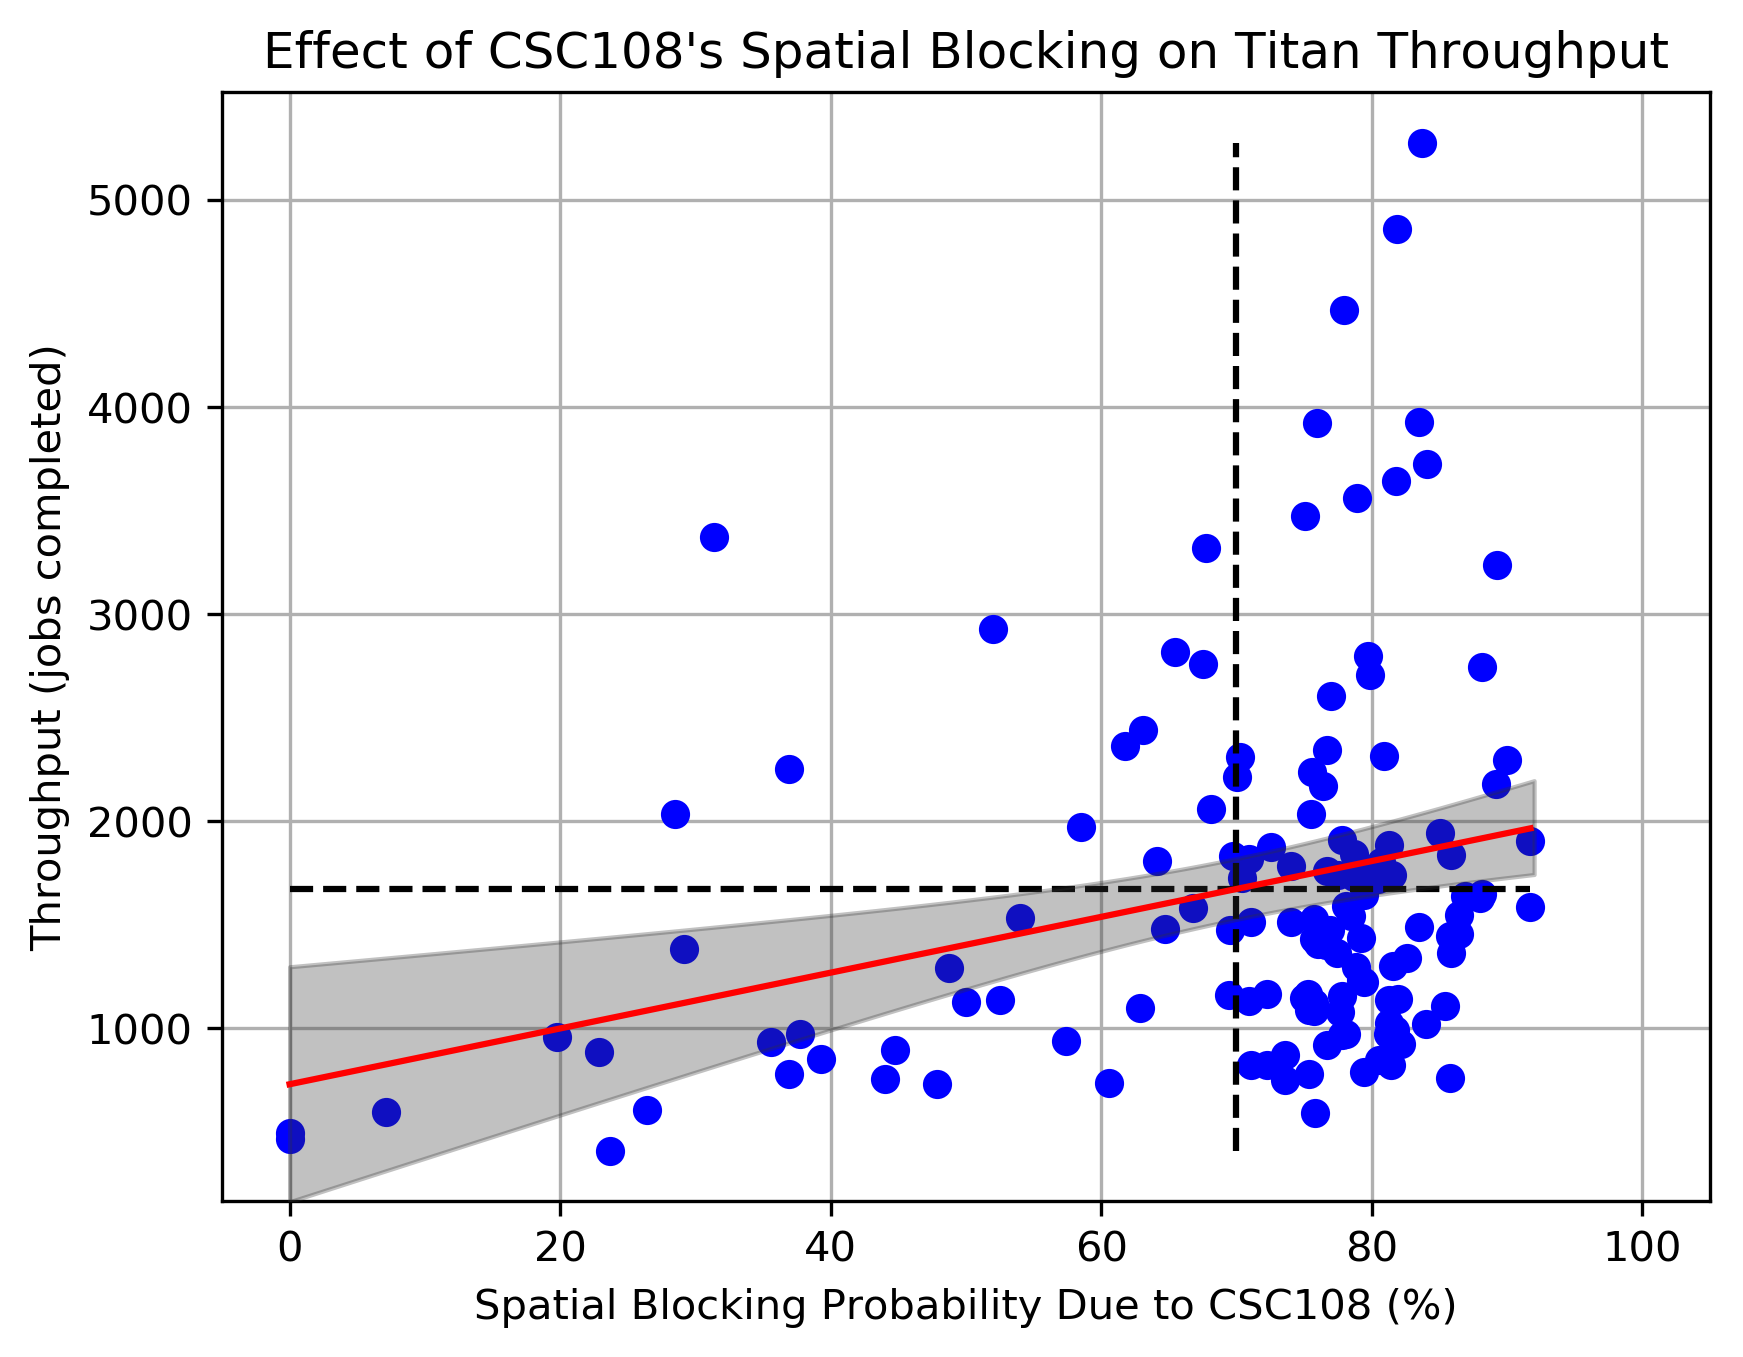
\includegraphics[width=0.4\textwidth]{images/linfit-throughput-vs-csc108-spatial.png}}
  \subfloat[Temporal blocking by CSC108\label{fig:throughput-temporal-csc108}]{
    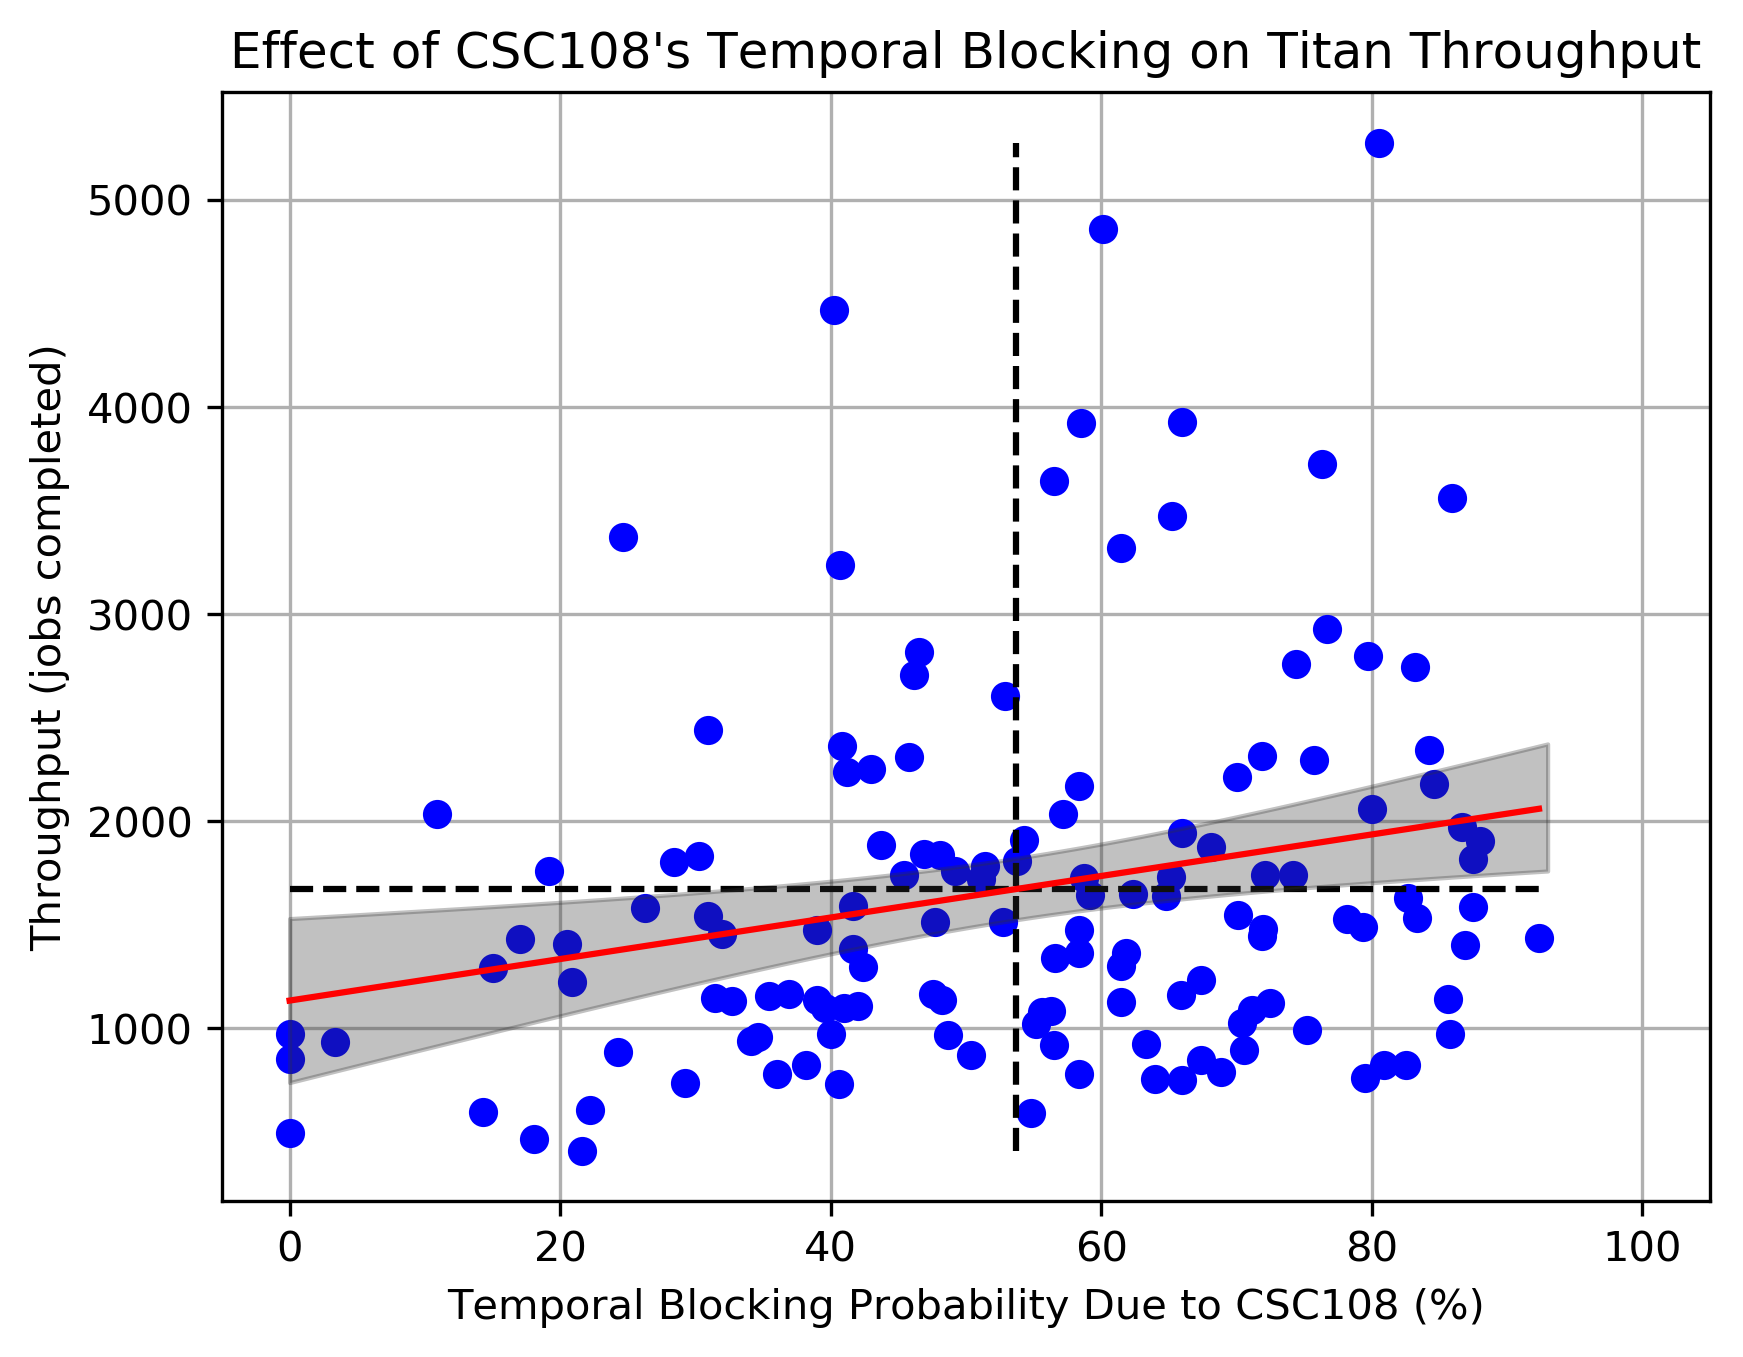
\includegraphics[width=0.4\textwidth]{images/linfit-throughput-vs-csc108-temporal.png}}
  \caption{These plots demonstrate the relationships between throughput on
Titan and one-dimensional blocking probabilities. Each blue point represents
one day. Each red line is an Ordinary Least Squares (OLS) linear regression
with parameters given in Table~\ref{tab:blocking-throughput-params}. Each
shaded gray area represents a 95\% confidence region. Each horizontal dotted
black line represents the mean wait times for all points in that plot, and each
vertical dotted black line represents the mean blocking probability for all
points in that plot.}
\end{figure*}

% For tables use
\begin{table}
% table caption is above the table
\caption{The table contains the parameter values for the Ordinary Least Squares
(OLS) linear regression models regarding blocking probabilities and throughput.
The first column corresponds to the figure depicting the model, while the
second and third columns correspond the coefficients $\beta_1$ and $\beta_0$ in
the model $y = \beta_{1}x + \beta_0$.}
\label{tab:blocking-throughput-params}       % Give a unique label
% For LaTeX tables use
\begin{tabular}{crrr}
\hline\noalign{\smallskip}
Figure  & Slope $\beta_1$ & Intercept $\beta_0$     & $\text{R}^2$ \\
\noalign{\smallskip}\hline\noalign{\smallskip}
\ref{fig:throughput-spatial-all}     &  16.2402 &   252.3652    &   0.0122  \\
\ref{fig:throughput-temporal-all}    &   1.7196 &  1544.9669    &   0.0010  \\
\ref{fig:throughput-spatial-csc108}  &  13.4683 &   730.0687    &   0.0790  \\
\ref{fig:throughput-temporal-csc108} &  10.0245 &  1134.0212    &   0.0587  \\
\noalign{\smallskip}\hline
\end{tabular}
\end{table}
%%%

%%% UTILIZATION STUFF

Finally, we searched for simple linear relationships between the different
blocking probabilities and overall utilization on Titan. Figures
\ref{fig:utilization-spatial-all}, \ref{fig:utilization-temporal-all},
\ref{fig:utilization-spatial-csc108}, and \ref{fig:utilization-temporal-csc108}
do not ``agree'' like the throughput plots did, but three plots suggest an
interpretation in which increasing competition, indicated by increasing
blocking probability, corresponds to decreased utilization. The fourth plot,
which indicates competition with CSC108, relates increased competition to
increased utilization. Once again, the goodness-of-fit values are poor, as
shown in Table~\ref{tab:blocking-utilization-params}.

%%%
\begin{figure*}
  \subfloat[Spatial blocking\label{fig:utilization-spatial-all}]{
    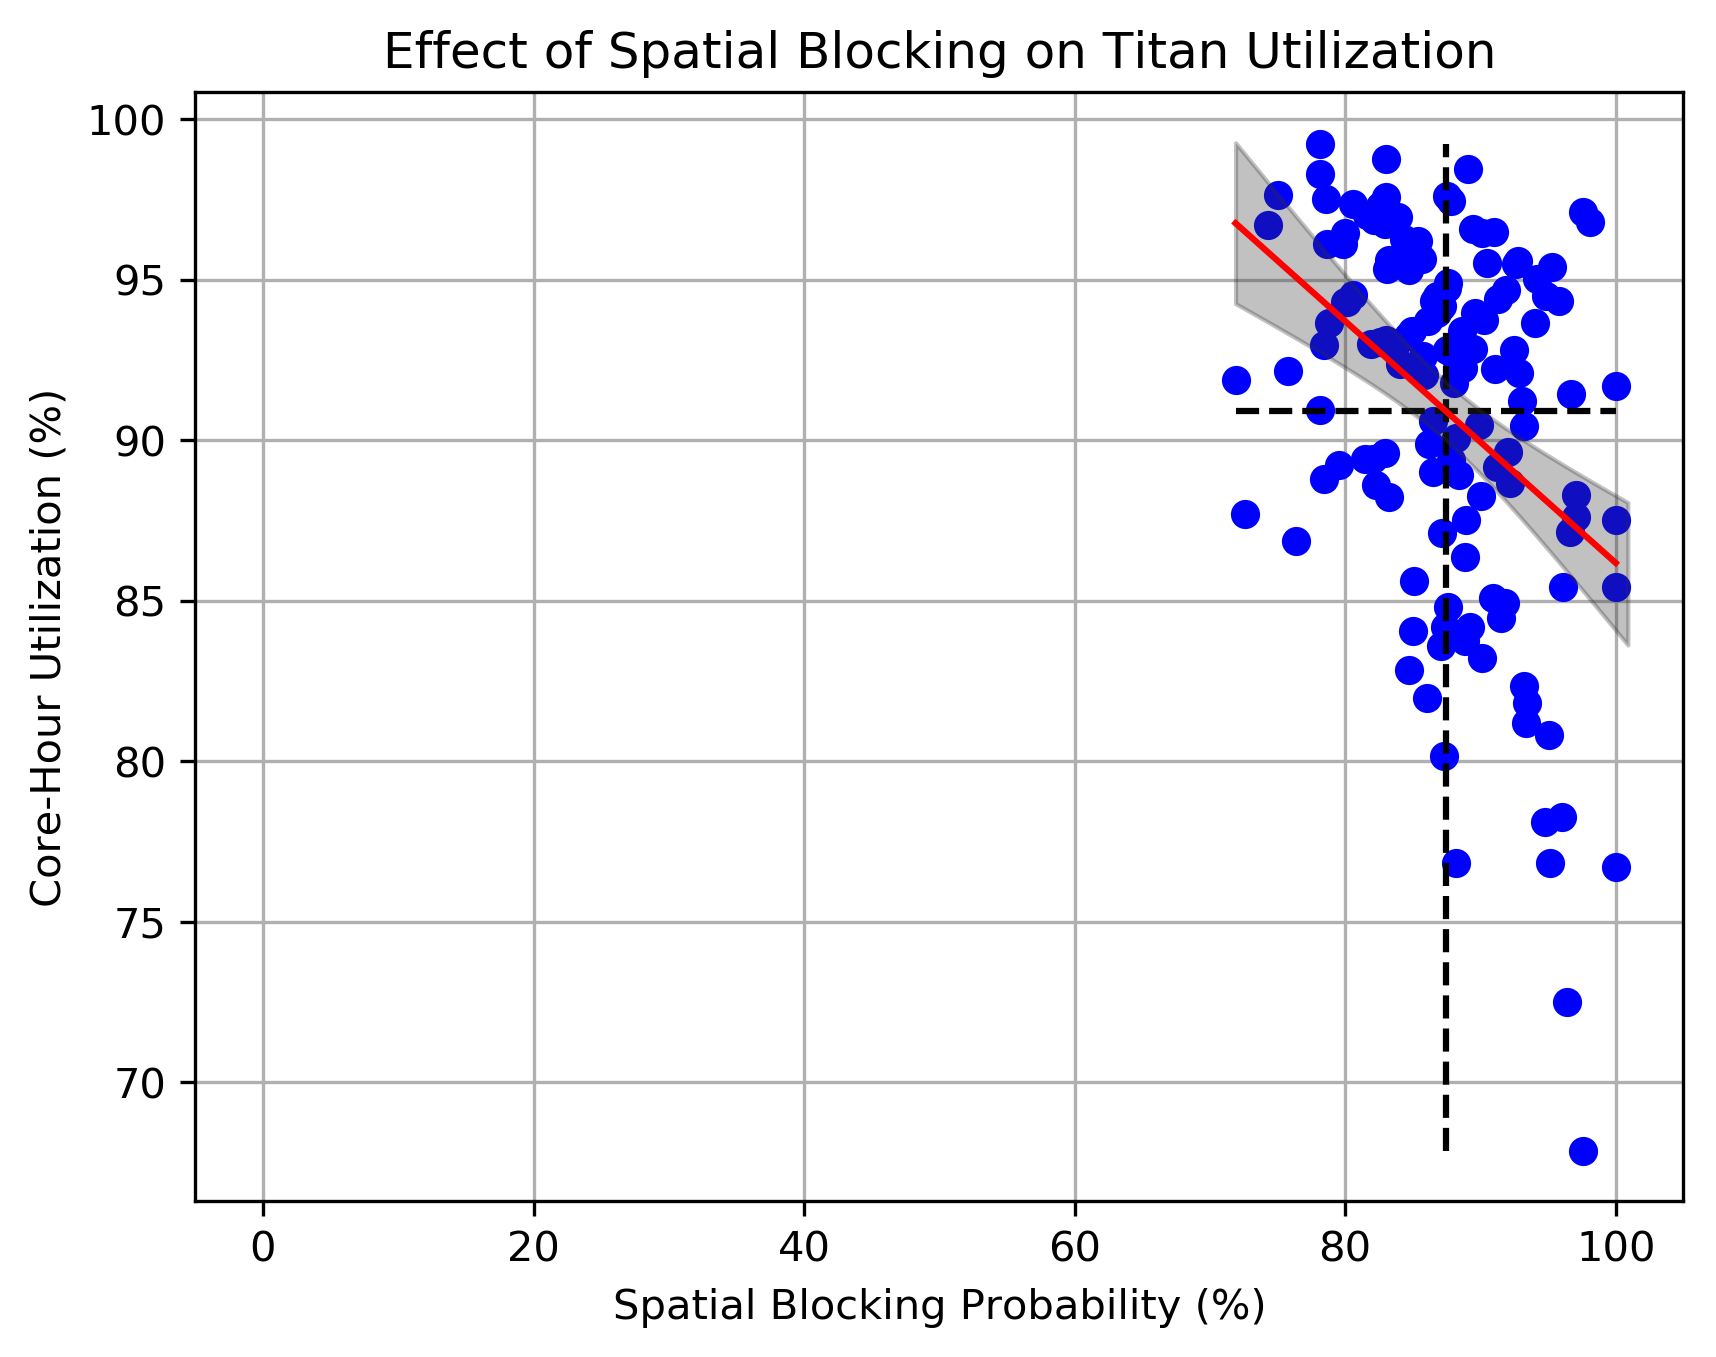
\includegraphics[width=0.4\textwidth]{images/linfit-utilization-vs-spatial-blocking.png}}
  \subfloat[Temporal blocking\label{fig:utilization-temporal-all}]{
    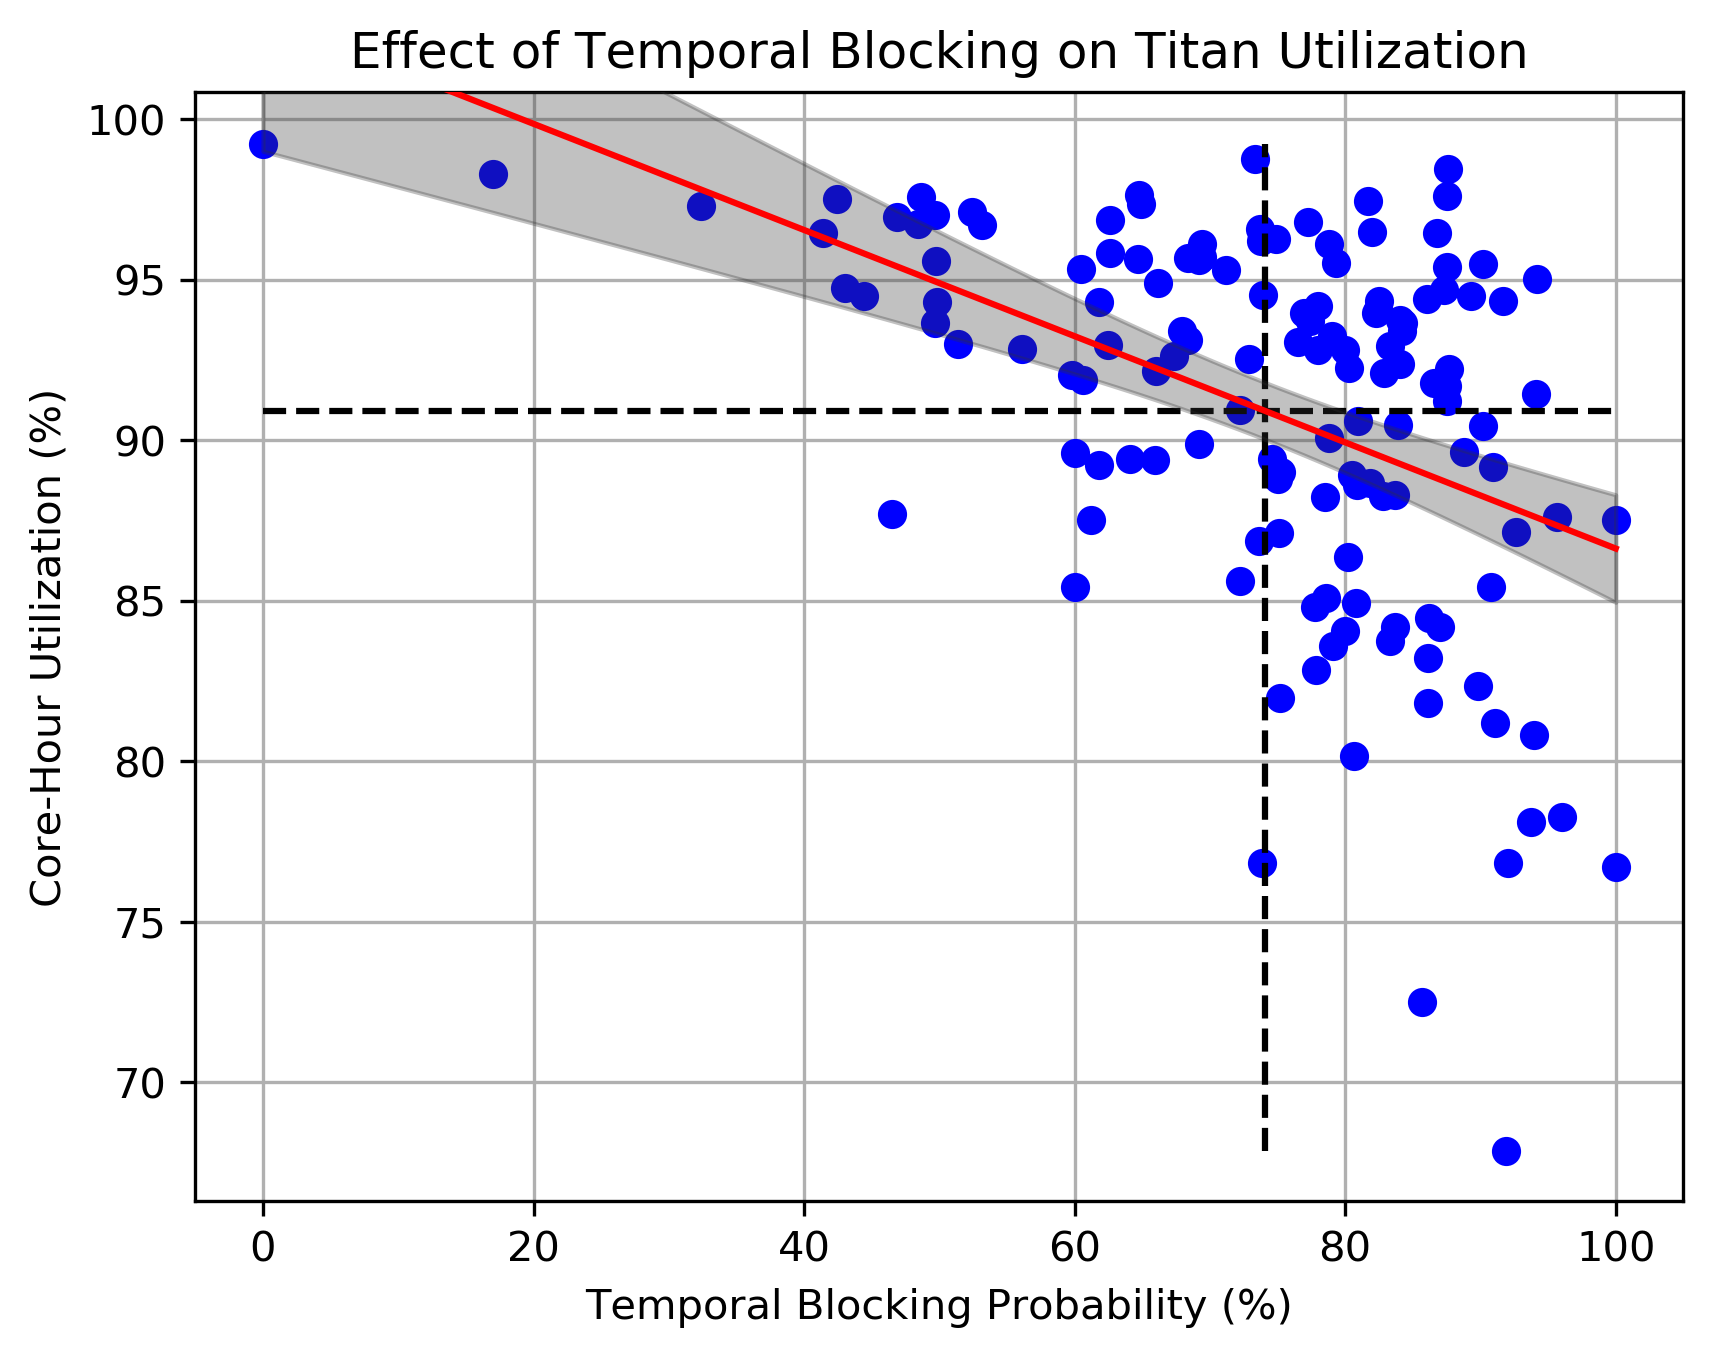
\includegraphics[width=0.4\textwidth]{images/linfit-utilization-vs-temporal-blocking.png}}
  \vspace{1em}
  \subfloat[Spatial blocking by CSC108\label{fig:utilization-spatial-csc108}]{
    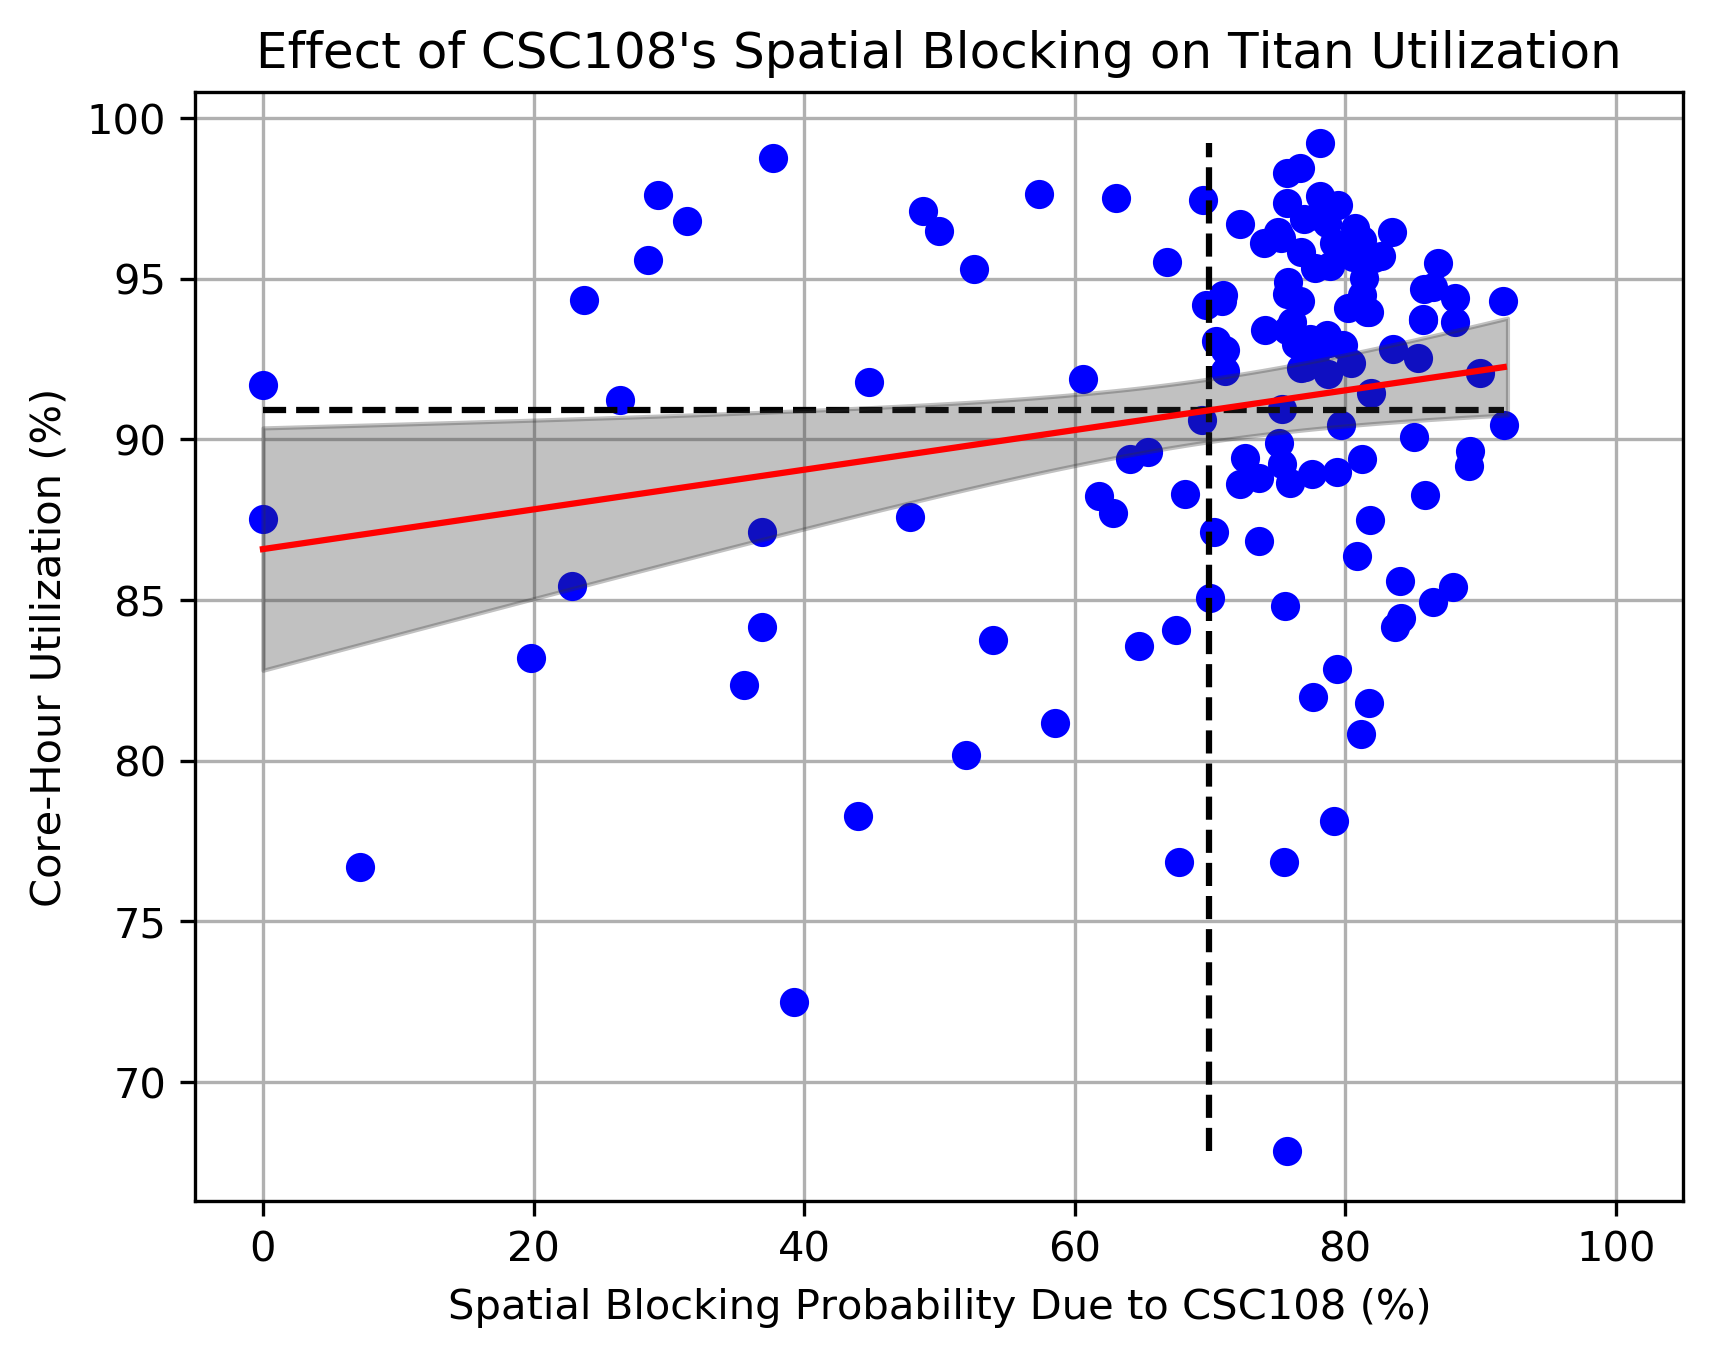
\includegraphics[width=0.4\textwidth]{images/linfit-utilization-vs-csc108-spatial.png}}
  \subfloat[Temporal blocking by CSC108\label{fig:utilization-temporal-csc108}]{
    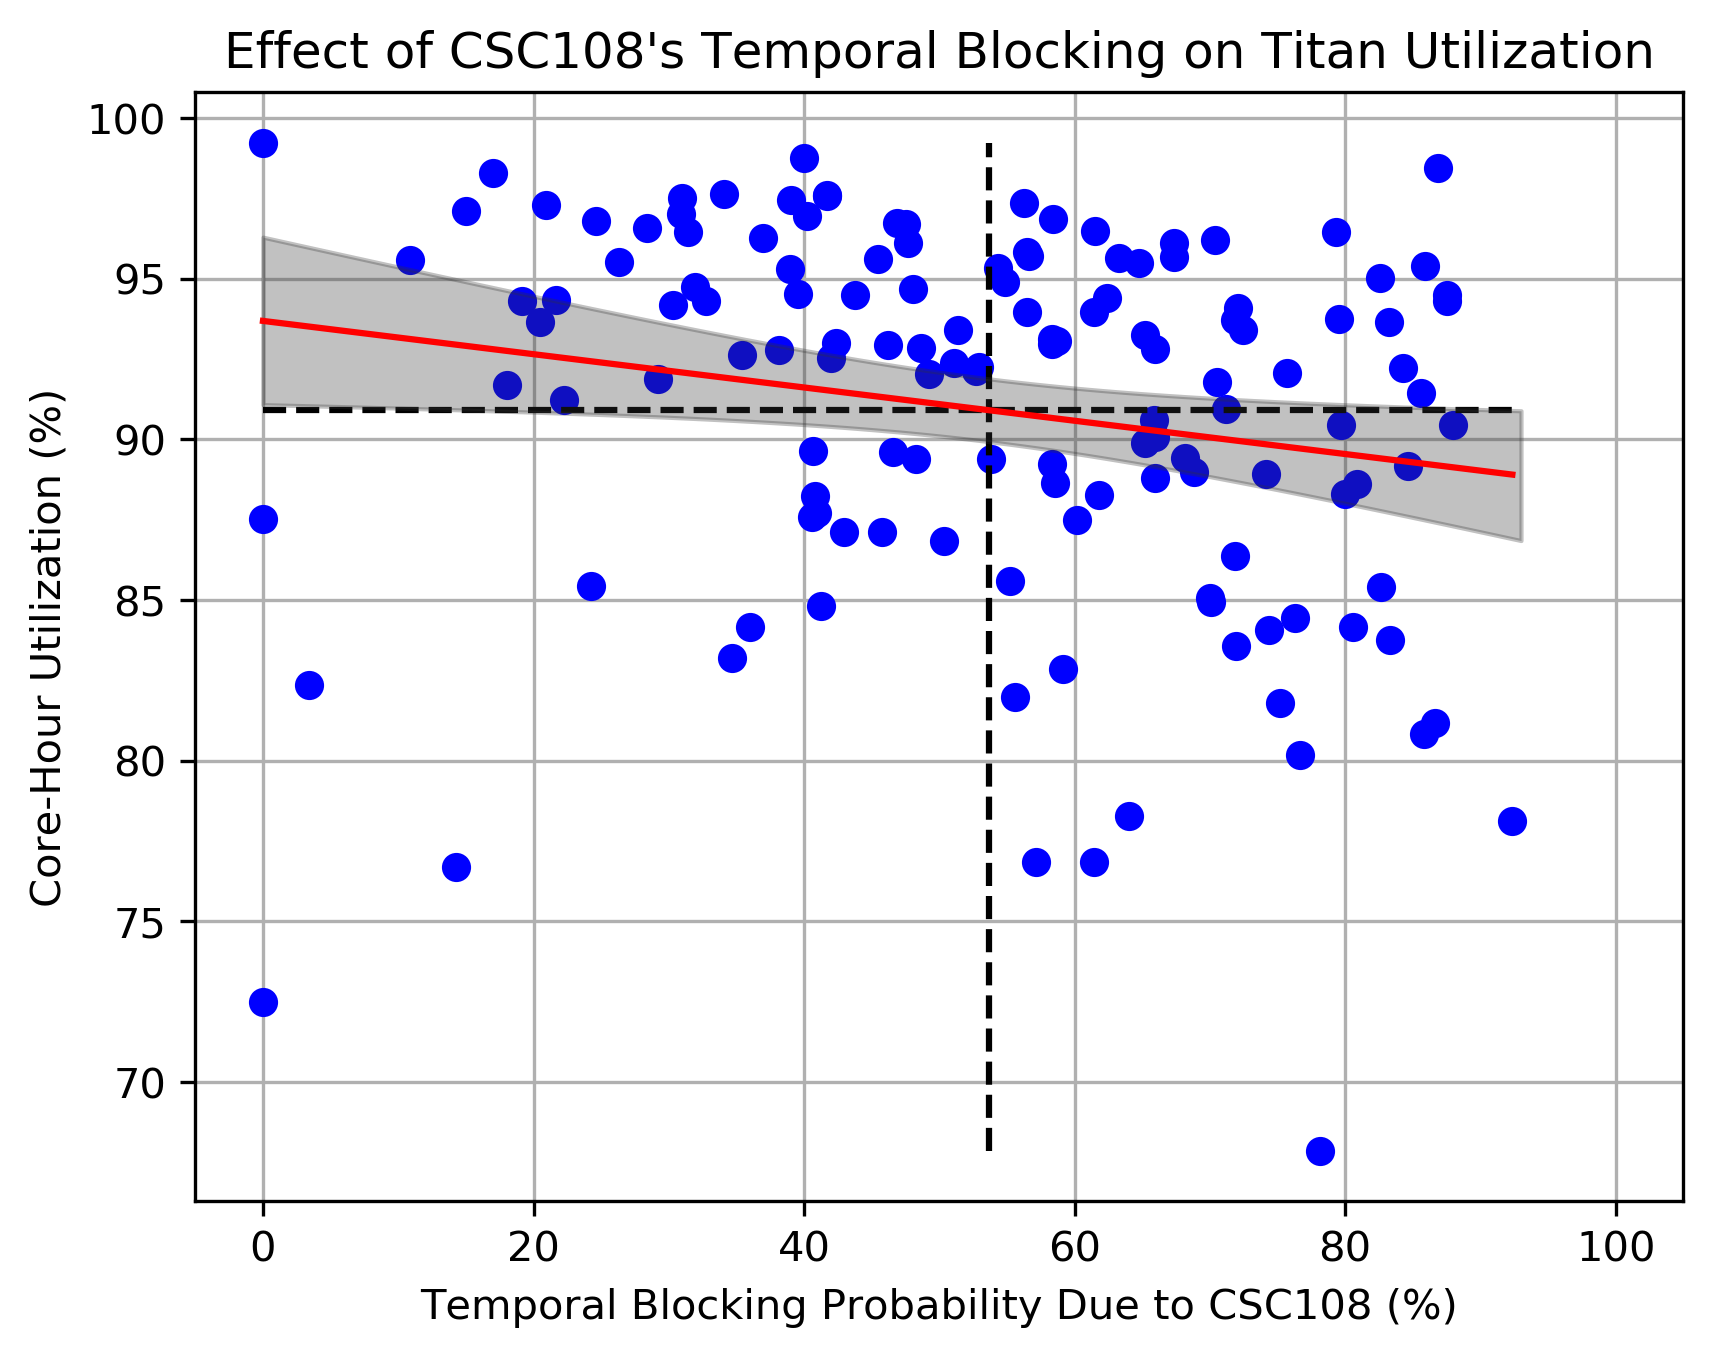
\includegraphics[width=0.4\textwidth]{images/linfit-utilization-vs-csc108-temporal.png}}
  \caption{These plots demonstrate the relationships between utilization on
Titan and one-dimensional blocking probabilities. Each blue point represents
one day. Each red line is an Ordinary Least Squares (OLS) linear regression
with parameters given in Table~\ref{tab:blocking-utilization-params}. Each
shaded gray area represents a 95\% confidence region. Each horizontal dotted
black line represents the mean wait times for all points in that plot, and each
vertical dotted black line represents the mean blocking probability for all
points in that plot.}
\end{figure*}

% For tables use
\begin{table}
% table caption is above the table
\caption{The table contains the parameter values for the Ordinary Least Squares
(OLS) linear regression models regarding blocking probabilities and utilization.
The first column corresponds to the figure depicting the model, while the
second and third columns correspond the coefficients $\beta_1$ and $\beta_0$ in
the model $y = \beta_{1}x + \beta_0$.}
\label{tab:blocking-utilization-params}       % Give a unique label
% For LaTeX tables use
\begin{tabular}{crrr}
\hline\noalign{\smallskip}
Figure  & Slope $\beta_1$ & Intercept $\beta_0$     & $\text{R}^2$ \\
\noalign{\smallskip}\hline\noalign{\smallskip}
\ref{fig:utilization-spatial-all}       &   -0.3766 &   123.8332 & 0.1543 \\
\ref{fig:utilization-temporal-all}    &     -0.1654 &   103.1603 & 0.2084 \\
\ref{fig:utilization-spatial-csc108}  &      0.0617 &    86.5830 & 0.0391 \\
\ref{fig:utilization-temporal-csc108} &     -0.0518 &    93.6845 & 0.0370 \\
\noalign{\smallskip}\hline
\end{tabular}
\end{table}
%%%

Thus, the use of blocking probability provided additional insight regarding the
impact of CSC108 on Titan, but just like in
Section~\ref{subsec:simple-linear-relationships}, the best-fit lines all
displayed very poor goodness-of-fit, rendering the interpretations somewhat
weak.

%-  vim:set syntax=tex:


% ---------------------------------------------------------------------------
% V - Workload Management for HPC Beyond ATLAS and OLCF
% ---------------------------------------------------------------------------

\section{HPC Workload Management beyond ATLAS and OLCF}
\label{sec:beyond-atlas-and-olcf}
%-  LaTeX source file

%-  section5.tex ~~
%
%   This contains what was originally the seventh section of the Google Docs
%   draft of the paper.
%
%                                                   ~~ last updated 18 Jan 2019

The objective of each subsection is to:
(i) describe the science; and
(ii) detail what customizations had to be done -- either on PanDA or the Titan
    end to support the science driver.
We will then conclude this section with a summary.

\subsection{PanDA WMS beyond HEP}
\label{subsec:panda_beyond}

Traditionally computing in physics experiments at the basic level is usually
independent processing of the input files to produce the output. This
processing in referring in the paper as a job. Processing algorithm usually
utilizes some experiment-specific software which may require parameterization
and even additional configuration files. In the case if such a configuration
file is specific for each job it can be defined in a job as another input file.
Also experiment software may produce some additional files along with the
primary output and they need to be stored. For instance PanDA pilot itself
produces the tar-archive file containing the logs its own logs and the
experiments software logs. Processing algorithm (referenced as ``transformation
script'') responsible for the correct launching the experiment software and
provide all necessary input information including the configuration and run
parameters. PanDA job definition is only defines the launching command for the
transformation script. This launching command is referring as a payload.

The following components are usually provided and controlled by the experiment groups outside from PanDA core components.
\begin{itemize}
    \item Transformation scripts. User groups should define a complete set of
        the transformations scripts to cover all possible SW usage. In the case
        if the same software is used and only the run parameters, configuration
        and input/output file names are changing, the single transformation
        script should be able to cope this.
    \item Input/output files conventions. The size of the input files often
        adjusted in a way to balance of the total processing walltime and
        flexibility in order to cope the failure risks. There is often case
        that the equal sized input files are required relatively equal
        processing time and produce equal sized output. Also input files are
        often named conventionally and grouped in the datasets by some
        attributes. PanDA job definition allows to provide name for the
        input/output datasets.
\end{itemize}

The real workflow for each scientific group provides a lot of additional
requirements and constraints. A common example is a specific order of the jobs
execution. Also implementation of the dedicated workflows demands an
integration with existing experiment computing infrastructure or even
development an additional components. This includes the issues with data
management, user authentication, monitoring, workflow control and etc.

PanDA system may be the best solution for the new experiments and scientific
groups by diversity of provided advantages. The main motivations for users are:
\begin{itemize}
    \item Powerful workload management. Automation of the jobs handling,
        monitoring and logging.
    \item Streamlining the usage of the computing resources. Possibility for
        users to run their jobs on diversity of the computing resources. Local
        resource schedulers, and policies are transparent for the users.
    \item PanDA native data handling. PanDA provides a diverse set of the
        plugins to support data stage-in/-out from the remote storages and
        different data movement tools of different types.
    \item Close integration with OLCF. Being integrated with OLCF PanDA system
        also became attractive for many scientific groups already utilizing
        OLCF resources or those who wish to get use them. 
\end{itemize}

Currently, there are few PanDA instances in use by different experiments and
groups.  In this paper, we have considered three instances. The original
instance is installed at CERN, and it is used exclusively for the ATLAS
experiment. Another instance is installed at OLCF, and it is dedicated to
supporting projects on Titan, subject to OLCF policies. Finally, an instance on
Amazon's EC2 cloud infrastructure provides access to multiple independent
experiments from different disciplines, and it has the least restrictive
security and usage policies.

\subsection{PanDA instance at OLCF}
\label{subsec:panda_instance}

In March 2017, we implemented a new PanDA server instance within OLCF operating
under Red Hat OpenShift Origin \cite{RH_OpenShift} - a powerful container
cluster management and orchestration system in order to serve various
experiments at Titan supercomputer. By running on-premise Red Hat OpenShift
built on Kubernetes \cite{Kubernetes}, the OLCF provides a container
orchestration service that allows users to schedule and run their HPC
middleware service containers while maintaining a high level of support for
many diverse service workloads. The containers have direct access to all OLCF
shared resources such as parallel filesystems and batch schedulers. With this
PanDA instance, we implemented a set of demonstrations serving diverse
scientific workflows including physics, biology studies of the genes and human
brain, and molecular dynamics studies:

\begin{itemize}
    \item Biology / Genomics. 
In collaboration with Center for Bioenergy Innovation at ORNL the PanDA based
workflow for epistasis researches was established. Epistasis is the phenomenon
where the effect of one gene is dependent on the presence of one or more
``modifier genes'', i.e. the genetic background. GBOOST \cite{GBOOST} is a
GPU-based tool for detecting gene-gene interactions in genome-wide case control
studies, was used for initial tests.

    \item Molecular Dynamics.
In collaboration with the Chemistry and Biochemistry department of the
University of Texas Arlington, we implemented a test to try out PanDA to
support the Molecular Dynamics study ``Simulating Enzyme Catalysis,
Conformational Change, and Ligand Binding/Release''. The CHARMM (Chemistry at
HARvard Macromolecular Mechanics) \cite{Brooks2009CHARMM} a molecular
simulation program was chosen as a basic payload tool. CHARMM design for hybrid
MPI/OpenMP/GPU computing.

    \item IceCube. 
Together with experts from the IceCube experiment we implemented the
demonstrator PanDA system. IceCube \cite{Halzen:2010yj} is a particle detector
at the South Pole that records the interactions of a nearly massless subatomic
particle called the neutrino. Demonstrator includes the use of NuGen package (a
modified version of ANIS \cite{Gazizov:2004va} that works with IceCube
software) - GPU application for atmospheric neutrinos are simulations packed in
Singularity container and remote stage-in/-out the data from GridFTP
\cite{Allcock:2005:GSG:1105760.1105819} storage with GSI authentication. 

    \item BlueBrain.
In 2017, a R\&D project was started between BigPanDA and the Blue Brain Project
(BBP) \cite{Markram} of the Ecole Polytechnique Federal de Lausanne (EPFL)
located in Lausanne, Switzerland. This proof of concept project is aimed at
demonstrating the efficient application of the BigPanDA system to support the
complex scientific workflow of the BBP which relies on using a mix of desktop,
cluster, and supercomputers to reconstruct and simulate accurate models of
brain tissue. In the first phase of this joint project we supported the
execution of BBP software on a variety of distributed computing systems powered
by BigPanDA. The targeted systems for demonstration included: Intel x86-NVIDIA
GPU based BBP clusters located in Geneva (47 TFlops) and Lugano (81 TFlops),
BBP IBM BlueGene/Q supercomputer \cite{citeulike:472727} (0.78 PFLops and 65 TB
of DRAM memory) located in Lugano, the Titan Supercomputer with peak
theoretical performance 27 PFlops operated by the Oak Ridge Leadership
Computing Facility (OLCF), and Cloud based resources such as Amazon Cloud.

    \item LSST.
A goal of LSST (Large Synoptic Survey Telescope) project is to conduct a
10-year survey of the sky that is expected to deliver 200 petabytes of data
after it begins full science operations in 2022. The project  will address some
of the most pressing questions about the structure and evolution of the
universe and the objects in it. It will require a large amount of simulations,
which model the atmosphere, optics and camera to understand the collected data.
For running LSST simulations with the PanDA WMS we have established a
distributed testbed infrastructure that employs the resources of several sites
on GridPP \cite{0954-3899-32-1-N01} and Open Science Grid (OSG)
\cite{1742-6596-78-1-012057} as well as the Titan supercomputer at ORNL. In
order to submit jobs to these sites we have used a PanDA server instance
deployed on the Amazon AWS Cloud.

    \item LQCD.
Lattice QCD (LQCD) \cite{Babich:2010:PQL:1884643.1884695} is a well-established
non-perturbative approach to solving the quantum chromodynamics theory of
quarks  and gluons. Current LQCD payloads can be characterized as massively
parallel,  occupying thousands of nodes on leadership-class supercomputers.

In 2017, as a part of SciDAC-4 funded project, a collaboration was formed
between several US LQCD groups and BigPanDA team with the goal to adopt PanDA
WMS for the needs of the SciDAC-4 LQCD computational program. 

LQCD payloads have been successfully tested on Titan as well as on other sites.
%In order to run LQCD payloads we have also used our PanDA Server in Amazon
%cloud.
Production campaigns were executed on BNL Institutional Cluster through a
dedicated instance of Harvester installed on the front node of this site.
During the period between April and June 2018 13 TB of input data were
processed, producing output of 176 GB. LQCD jobs used around 15,000 GPU hours
with average job duration around 12 hours.

    \item nEDM.
Precision measurements of the properties of the neutron present an opportunity
to search for violations of fundamental symmetries and to make critical tests
of the validity of the Standard Model of electroweak interactions. These
experiments have been pursued \cite{Sakharov:1967dj} with great energy and
interest since the discovery of neutron in 1932. The goal of the nEDM
\cite{0954-3899-36-10-104002} experiment at the Fundamental Neutron Physics
Beamline at the Spallation Neutron Source (Oak Ridge National Laboratory) is to
further improve the precision of this measurement by another factor of 100.
\end{itemize}

To isolate the workflows of different groups and experiments, dedicated queues
were defined at the PanDA server. Presumably in  next steps we will provide the
security mechanisms that will provide the access to each queue for job
submission and dispatching only for authorised users. Also, the PanDA server
provides the tools to customise environment variables, system settings and
workflow algorithms for different user groups. Also this split of the different
groups workflows on the level of PanDA queues simplifies jobs monitoring via
the web based PanDA tool. 

In collaboration with the dedicated scientific groups representatives, we
implemented the ``transformation'' scripts containing complete definition of
the processing actions (set of specific software and general system commands)
are has to be applied to the input data to produce the output. The
transformation script then can be addressed by its name. Client tool provided
to the users allows to submit jobs to the PanDA server with authentication
based on grid certificates. 

Responsible group representative also authorized to run pilots launcher daemon.
Daemon launches the pilots. Number of parallel running pilots can be
configured. Pilots are running and interacts with the PBS under user account
and with Titan group privileges of the responsible representative.

The most important parameters of conducted tests are presented in the table

% For tables use
\begin{table}
% table caption is above the table
\caption{Please write your table caption here}
\label{tab:beyondhep}       % Give a unique label
% For LaTeX tables use
\begin{tabular}{llrrrrr}
\hline\noalign{\smallskip}
% ORIGINAL COLUMN TITLES:
%Experiment & Payload/SW & Number of jobs per campaign & Number of nodes per
%job & Walltime (min) & Input data size per job & Output data size per job \\
Experiment & Payload & Jobs & Nodes & Walltime & Input data & Output data \\
\noalign{\smallskip}\hline\noalign{\smallskip}
Genomics           & GBOOST & 10    & 2    & 30 min    & 100 MB & 300 MB \\
Molecular Dynamics & CHARMM & 10    & 124  & 30-90 min & 10 KB  & 2-6 GB \\
IceCube            & NuGen  & 4500K & 1    & 120 min   & 500 KB & 10KB - 4GB \\
LSST/DESC          & Phosim & 20    & 2    & 600 min   & 700 MB & 70 MB \\
LQCD               & QDP++  & 10    & 8000 & 700 min   & 40 GB  & 150 MB \\
nEDM               & GEANT  & 10    & 200  & 20 min    & 120 MB & 20 MB \\
\noalign{\smallskip}\hline
\end{tabular}
\end{table}


\subsection{Summary}
\label{subsec:summary}

The overview of the successfully implemented demonstrations of diverse
workflows implementation via PanDA shows that PanDA model can cope the
challenges of the different experiments and user groups and also provide
possibility for extensions beyond the core components set.  The proof of
concept was received from all considered experiments representatives and
results that PanDA is considered as a possible solution. Preproduction
utilization of PanDA is now under investigation with BlueBrain, IceCube, LSST,
nEDM experiments, LQCD uses PanDA for Production.

%-  vim:set syntax=tex:


%%%

% ---------------------------------------------------------------------------
% VI - Summary
% ---------------------------------------------------------------------------

\section{Summary}
\label{sec:summary}
%-  LaTeX source file

%-  section6.tex ~~
%                                                   ~~ last updated 16 Sep 2019



%-  vim:set syntax=tex:


%%%

%% For one-column wide figures use
%\begin{figure}
%% Use the relevant command to insert your figure file.
%% For example, with the graphicx package use
%  
\includegraphics{images/example.eps}
%% figure caption is below the figure
%\caption{Please write your figure caption here}
%\label{fig:1}       % Give a unique label
%\end{figure}
%%
%% For two-column wide figures use
%\begin{figure*}
%% Use the relevant command to insert your figure file.
%% For example, with the graphicx package use
%  
\includegraphics[width=0.75\textwidth]{images/example.eps}
%% figure caption is below the figure
%\caption{Please write your figure caption here}
%\label{fig:2}       % Give a unique label
%\end{figure*}
%%
%

\begin{acknowledgements}
    This work is funded by Award number DESC0016280 from the Office of Advanced
    Scientific Computing Research within the Department of Energy. This
    research used resources of the Oak Ridge Leadership Computing Facility at
    the Oak Ridge National Laboratory, which is supported by the Office of
    Science of the U.S. Department of Energy under Contract
    No.\ DE-AC05-00OR22725.
\end{acknowledgements}


%-  NOTE: I (Sean) chose the bibliography style arbitrarily.

%\bibliographystyle{spbasic}      % basic style, author-year citations
%\bibliographystyle{spmpsci}      % mathematics and physical sciences
\bibliographystyle{spphys}       % APS-like style for physics
\bibliography{bibliography,radical_publications}


%-  That's all, folks!

\end{document}

%-  vim:set syntax=tex:
